% ******************************* PhD Thesis Template **************************
% Please have a look at the README.md file for info on how to use the template

\documentclass[a4paper,12pt,times,numbered,print,index]{Classes/PhDThesisPSnPDF}


% ******************************************************************************
% ******************************* Class Options ********************************
% *********************** See README for more details **************************
% ******************************************************************************

% `a4paper'(The University of Cambridge PhD thesis guidelines recommends a page
% size a4 - default option) or `a5paper': A5 Paper size is also allowed as per
% the Cambridge University Engineering Deparment guidelines for PhD thesis
%
% `11pt' or `12pt'(default): Font Size 10pt is NOT recommended by the University
% guidelines
%
% `oneside' or `twoside'(default): Printing double side (twoside) or single
% side.
%
% `print': Use `print' for print version with appropriate margins and page
% layout. Leaving the options field blank will activate Online version.
%
% `index': For index at the end of the thesis
%
% `draftclassic': For draft mode without loading any images (same as draft in book)
%
% `draft': Special draft mode with line numbers, images, and water mark with
% timestamp and custom text. Position of the text can also be modified.
%
% `abstract': To generate only the title page and abstract page with
% dissertation title and name, to submit to the Student Registry
%
% `chapter`: This option enables only the specified chapter and it's references
%  Useful for review and corrections.
%
% ************************* Custom Page Margins ********************************
%
% `custommargin`: Use `custommargin' in options to activate custom page margins,
% which can be defined in the preamble.tex. Custom margin will override
% print/online margin setup.
%
% *********************** Choosing the Fonts in Class Options ******************
%
% `times' : Times font with math support. (The Cambridge University guidelines
% recommend using times)
%
% `fourier': Utopia Font with Fourier Math font (Font has to be installed)
%            It's a free font.
%
% `customfont': Use `customfont' option in the document class and load the
% package in the preamble.tex
%
% default or leave empty: `Latin Modern' font will be loaded.
%
% ********************** Choosing the Bibliography style ***********************
%
% `authoryear': For author-year citation eg., Krishna (2013)
%
% `numbered': (Default Option) For numbered and sorted citation e.g., [1,5,2]
%
% `custombib': Define your own bibliography style in the `preamble.tex' file.
%              `\RequirePackage[square, sort, numbers, authoryear]{natbib}'.
%              This can be also used to load biblatex instead of natbib
%              (See Preamble)
%
% **************************** Choosing the Page Style *************************
%
% `default (leave empty)': For Page Numbers in Header (Left Even, Right Odd) and
% Chapter Name in Header (Right Even) and Section Name (Left Odd). Blank Footer.
%
% `PageStyleI': Chapter Name next & Page Number on Even Side (Left Even).
% Section Name & Page Number in Header on Odd Side (Right Odd). Footer is empty.
%
% `PageStyleII': Chapter Name on Even Side (Left Even) in Header. Section Number
% and Section Name in Header on Odd Side (Right Odd). Page numbering in footer


% ********************************** Preamble **********************************
% Preamble: Contains packages and user-defined commands and settings
% ******************************************************************************
% ****************************** Custom Margin *********************************

% Add `custommargin' in the document class options to use this section
% Set {innerside margin / outerside margin / topmargin / bottom margin}  and
% other page dimensions
\ifsetCustomMargin
  \RequirePackage[left=37mm,right=30mm,top=35mm,bottom=30mm]{geometry}
  \setFancyHdr % To apply fancy header after geometry package is loaded
\fi

% Add spaces between paragraphs
%\setlength{\parskip}{0.5em}
% Ragged bottom avoids extra whitespaces between paragraphs
\raggedbottom
% To remove the excess top spacing for enumeration, list and description
%\usepackage{enumitem}
%\setlist[enumerate,itemize,description]{topsep=0em}

% *****************************************************************************
% ******************* Fonts (like different typewriter fonts etc.)*************

% Add `customfont' in the document class option to use this section

\ifsetCustomFont
  % Set your custom font here and use `customfont' in options. Leave empty to
  % load computer modern font (default LaTeX font).
  %\RequirePackage{helvet}

  % For use with XeLaTeX
  %  \setmainfont[
  %    Path              = ./libertine/opentype/,
  %    Extension         = .otf,
  %    UprightFont = LinLibertine_R,
  %    BoldFont = LinLibertine_RZ, % Linux Libertine O Regular Semibold
  %    ItalicFont = LinLibertine_RI,
  %    BoldItalicFont = LinLibertine_RZI, % Linux Libertine O Regular Semibold Italic
  %  ]
  %  {libertine}
  %  % load font from system font
  %  \newfontfamily\libertinesystemfont{Linux Libertine O}
\fi

% *****************************************************************************
% **************************** Custom Packages ********************************

% ************************* Algorithms and Pseudocode **************************

%\usepackage{algpseudocode}


% ********************Captions and Hyperreferencing / URL **********************

% Captions: This makes captions of figures use a boldfaced small font.
%\RequirePackage[small,bf]{caption}

\RequirePackage[labelsep=space,tableposition=top]{caption}
\renewcommand{\figurename}{Fig.} %to support older versions of captions.sty


% *************************** Graphics and figures *****************************

%\usepackage{rotating}
%\usepackage{wrapfig}

% Uncomment the following two lines to force Latex to place the figure.
% Use [H] when including graphics. Note 'H' instead of 'h'
%\usepackage{float}
%\restylefloat{figure}

% Subcaption package is also available in the sty folder you can use that by
% uncommenting the following line
% This is for people stuck with older versions of texlive
%\usepackage{sty/caption/subcaption}
\usepackage{subcaption}

% ********************************** Tables ************************************
\usepackage{booktabs} % For professional looking tables
\usepackage{multirow}
\usepackage{array} % added 1901207 so that can set the width of table columns
\usepackage{multirow} % added 300117 so that can extend a row to include multiple rows

%\usepackage{multicol}
%\usepackage{longtable}
%\usepackage{tabularx}


% *********************************** SI Units *********************************
\usepackage{siunitx} % use this package module for SI units


% ******************************* Line Spacing *********************************

% Choose linespacing as appropriate. Default is one-half line spacing as per the
% University guidelines

% \doublespacing
% \onehalfspacing
% \singlespacing


% ************************ Formatting / Footnote *******************************

% Don't break enumeration (etc.) across pages in an ugly manner (default 10000)
%\clubpenalty=500
%\widowpenalty=500

%\usepackage[perpage]{footmisc} %Range of footnote options


% *****************************************************************************
% *************************** Bibliography  and References ********************

%\usepackage{cleveref} %Referencing without need to explicitly state fig /table

% Add `custombib' in the document class option to use this section
\ifuseCustomBib
   \RequirePackage[square, sort, numbers, authoryear]{natbib} % CustomBib

% If you would like to use biblatex for your reference management, as opposed to the default `natbibpackage` pass the option `custombib` in the document class. Comment out the previous line to make sure you don't load the natbib package. Uncomment the following lines and specify the location of references.bib file

%\RequirePackage[backend=biber, style=numeric-comp, citestyle=numeric, sorting=nty, natbib=true]{biblatex}
%\bibliography{References/references} %Location of references.bib only for biblatex

\fi

% changes the default name `Bibliography` -> `References'
\renewcommand{\bibname}{References}


% ******************************************************************************
% ************************* User Defined Commands ******************************
% ******************************************************************************

% *********** To change the name of Table of Contents / LOF and LOT ************

%\renewcommand{\contentsname}{My Table of Contents}
%\renewcommand{\listfigurename}{My List of Figures}
%\renewcommand{\listtablename}{My List of Tables}


% ********************** TOC depth and numbering depth *************************

\setcounter{secnumdepth}{2}
\setcounter{tocdepth}{2}


% ******************************* Nomenclature *********************************

% To change the name of the Nomenclature section, uncomment the following line

%\renewcommand{\nomname}{Symbols}


% ********************************* Appendix ***********************************

% The default value of both \appendixtocname and \appendixpagename is `Appendices'. These names can all be changed via:

%\renewcommand{\appendixtocname}{List of appendices}
%\renewcommand{\appendixname}{Appndx}

% *********************** Configure Draft Mode **********************************

% Uncomment to disable figures in `draft'
%\setkeys{Gin}{draft=true}  % set draft to false to enable figures in `draft'

% These options are active only during the draft mode
% Default text is "Draft"
%\SetDraftText{DRAFT}

% Default Watermark location is top. Location (top/bottom)
%\SetDraftWMPosition{bottom}

% Draft Version - default is v1.0
%\SetDraftVersion{v1.1}

% Draft Text grayscale value (should be between 0-black and 1-white)
% Default value is 0.75
%\SetDraftGrayScale{0.8}


% ******************************** Todo Notes **********************************
%% Uncomment the following lines to have todonotes.

%\ifsetDraft
%	\usepackage[colorinlistoftodos]{todonotes}
%	\newcommand{\mynote}[1]{\todo[author=kks32,size=\small,inline,color=green!40]{#1}}
%\else
%	\newcommand{\mynote}[1]{}
%	\newcommand{\listoftodos}{}
%\fi

% Example todo: \mynote{Hey! I have a note}


% ************************ Thesis Information & Meta-data **********************
% Thesis title and author information, refernce file for biblatex
\input{thesis-info}

% ***************************** Abstract Separate ******************************
% To printout only the titlepage and the abstract with the PhD title and the
% author name for submission to the Student Registry, use the `abstract' option in
% the document class.

\ifdefineAbstract
 \pagestyle{empty}
 \includeonly{Declaration/declaration, Abstract/abstract}
\fi

% ***************************** Chapter Mode ***********************************
% The chapter mode allows user to only print particular chapters with references
% Title, Contents, Frontmatter are disabled by default
% Useful option to review a particular chapter or to send it to supervisior.
% To use choose `chapter' option in the document class

\ifdefineChapter
 \includeonly{Chapter3/chapter3}
\fi

% ******************************** Front Matter ********************************
\begin{document}

\frontmatter

\maketitle

% ******************************* Thesis Dedidcation ********************************

\begin{dedication} 

I would like to dedicate this thesis to my loving parents \dots

\end{dedication}


% ******************************* Thesis Declaration ***************************

\begin{declaration}

I hereby declare that except where specific reference is made to the work of 
others, the contents of this dissertation are original and have not been 
submitted in whole or in part for consideration for any other degree or 
qualification in this, or any other university. This dissertation is my own 
work and contains nothing which is the outcome of work done in collaboration 
with others, except as specified in the text and Acknowledgements. This 
dissertation contains fewer than 65,000 words including appendices, 
bibliography, footnotes, tables and equations and has fewer than 150 figures.

% Author and date will be inserted automatically from thesis.tex \author \degreedate

\end{declaration}


% ************************** Thesis Acknowledgements **************************

\begin{acknowledgements}      


And I would like to acknowledge ...


\end{acknowledgements}

% ************************** Thesis Abstract *****************************
% Use `abstract' as an option in the document class to print only the titlepage and the abstract.
\begin{abstract}
This is where you write your abstract ...
\end{abstract}


% *********************** Adding TOC and List of Figures ***********************

\tableofcontents

\listoffigures

\listoftables

% \printnomenclature[space] space can be set as 2em between symbol and description
%\printnomenclature[3em]

\printnomenclature

% ******************************** Main Matter *********************************
\mainmatter

%*******************************************************************************
%*********************************** First Chapter *****************************
%*******************************************************************************

\graphicspath{{Chapter1/Figs/}}

\chapter{Introduction}  %Title of the First Chapter

Globally, there are approximately 80-100 tropical storms each year. The greatest frequency is observed in the Western North Pacific (WNP), with an average of 26 per year since 1981 \citep{zhan2012seasonal}. From 1977-2011, China had the highest rate of landfalls globally, averaging 6.4 per year \citep{HironoriFudeyasu:178}. Not only does the West Pacific experience the greatest number of tropical storms and landfalls per year, but also the most intense and largest. Tropical storms can occur throughout the year in the West Pacific, but the most active season is June-November.

%********************************** %First Section  *************************************

\section{Characteristics of tropical cyclones}

A tropical storm is a low pressure system that forms over tropical or sub-tropical waters (i.e. 23.4$^{\circ}$N to  23.4$^{\circ}$S), with organised convection and winds at low levels circulating anti-clockwise in the northern hemisphere or clockwise in the southern hemisphere. 

\begin{figure}[h]
	\centering
	\noindent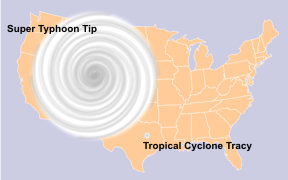
\includegraphics[width=15pc,angle=0]{typhoonsizes.jpg}
	\caption{Comparison of tropical cyclone sizes: Super Typhoon Tip and Tropical Cyclone Tracy. Source: \cite{noaa_structure}}\label{fig:cyclone_size}
\end{figure}

They are hugely variable in terms of size, illustrated in figure \ref{fig:cyclone_size}, where Tropical Cyclone Tracy (1974) covers just 0.03\% the area of Super Typhoon Tip (1979). Tropical cyclones tend to extend throughout the depth of the troposphere, approximately 16 km. The Saffir-Simpson Hurricane Scale \citep{simpson1974hurricane} is often used to categorise tropical storms by intensity based on maximum winds. Storms with winds of 38 mph (61 km/h, 33 knots) or less are called 'tropical depressions' and above this they are called 'tropical storms'. With increasing intensity there are categories 1 to 5 'hurricanes', with categories 3,4,5 referred to as 'major hurricanes'. In the West Pacific basin, if maximum sustained winds reach 64 knots (33 m/s, 74 mph) the term 'typhoon' is used, and a 'Super Typhoon' is if the maximum sustained winds are at least 130 knots (67 m/s, 150 mph).
The speed they move along the underlying surface, or 'translation speed' is around 10-15mph (10 knots), but can slower or as fast as 40 mph \citep{mo_tc}.  
%Size is not necessarily an indication of hurricane intensity. 


\subsection{Formation of tropical storms}

There are a number of environmental factors that need to be satisfied in order for a tropical storm to generate at a location. These are:
\begin{itemize}
	\item Presence of a convective system
	\item Non-negligible Coriolis force (at least 500 km, 300 miles) from the equator) \citep{noaaA15}
	\item Low wind shear (less than about 20 knots (10 m/s, 23 mph) \citep{noaaA15} 
	%	\item Enhanced vorticity
	\item Sufficient humidity in the mid-troposphere
	\item Warm ocean water of at least 26.5$^{\circ}$C throughout a sufficient depth (50m) (section 1.3.1)
	
\end{itemize}

Tropical cyclones cannot be generated spontaneously. To develop, they require a weakly organized system with sizeable spin and low level inflow. For tropical cyclogenesis to occur, there is a requirement for the Coriolis force to provide for near gradient wind balance to occur. Without the Coriolis force, the low pressure of the disturbance cannot be maintained. Large values of vertical wind shear disrupt the incipient tropical cyclone and can prevent genesis, therefore little wind shear is important. Relatively moist layers near the mid-troposphere (5 km, 3 miles). Dry mid levels are not conducive for allowing the continuing development of widespread thunderstorm activity. The development and maintenance of tropical cyclones require a warm ocean surface to act as a source of energy.

%Tory = enhanced cyclonic low-level vorticity .A pre-existing near-surface disturbance with sufficient vorticity and convergence. 
%Tropical waves spawn tcs... AEW, MT
%An atmosphere which cools fast enough with height such that it is potentially unstable to moist convection. 
%Tory - Tory - deep convection


\subsection{Tropical storm structure}

The main parts of a tropical cyclone are the dense cirrus overcast, rainbands, the eye, and the eyewall (figure \ref{fig:cyclone_structure}). There is boundary layer inflow in a cyclonic direction (anti-clockwise in the northern hemisphere) and anti-cyclonic (clockwise) upper tropospheric outflow.


\begin{figure}[h]
	\centering
	\noindent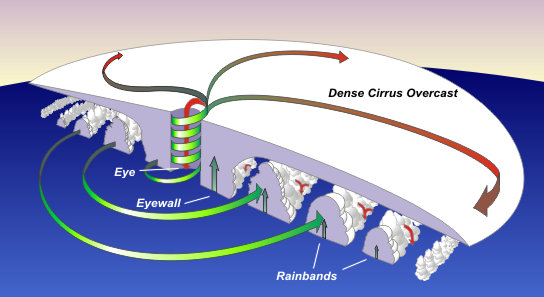
\includegraphics[width=20pc,angle=0]{hurr_cross.jpg}
	\caption{Tropical cyclone structure. Source: \cite{noaa_structure}}\label{fig:cyclone_structure}
\end{figure}

\subsubsection{Eye and eye wall}
The circular 'eye' or centre of a tropical cyclone is an area of slowly sinking air, characterised by light winds (usually do not exceed 15 mph (24 km/h)) \citep{noaa_structure} and little or no precipitation (figure \ref{fig:cyclone_structure}). Eye diameters are typically 40 km but can range from under 10 km to over 100 km \citep{bom_tc}. Although the winds are calm at the axis of rotation, strong winds may extend well into the eye. The eye is the region of lowest surface pressure and warmest temperatures aloft.

\begin{figure}[h]
	\centering
	\noindent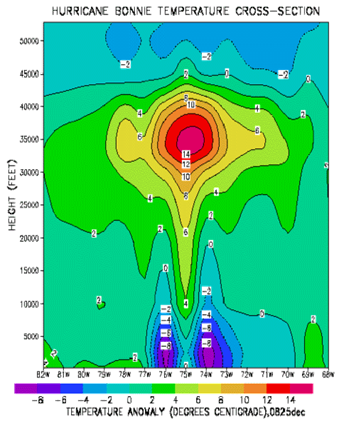
\includegraphics[width=14pc,angle=0]{warm_core2.png}
	\caption{Hurricane Bonnie temperature cross-section: the warm core. Source: \cite{eastin}}\label{fig:warm_core}
\end{figure}

Figure \ref{fig:warm_core} shows the maximum temperature anomalies present in the upper levels of the eye of Hurricane Bonnie. This is a result of subsidence and adiabatic heating in the eye, and eyewall latent heat release. The warm core is responsible for the extremely low surface pressures in the eye and large pressure gradients across the eyewall. The eye temperature may be 10$^{\circ}$C warmer or more at an altitude of 12 km (8 miles) than the surrounding environment, but only 0-2$^{\circ}$C warmer at the surface (Hawkins and Rubsam 1968) in the tropical cyclone (figure \ref{fig:warm_core}).

The eye is surrounded by a dense ring of cloud deep convection about 16 km high known as the eye wall which marks the belt of strongest winds and heaviest rainfall (\citep{bom_tc}). Changes in the structure of the eye and eyewall can cause affect the wind speed within the storm. The eye can grow or shrink in size, and double (concentric) eyewalls can form. In intense tropical cyclones, some of the outer rainbands may organize into an outer ring of thunderstorms that slowly moves inward. The inner eye wall (and storm intensity) weakens as it feels the effects of the subsidence resulting from this outer eyewall, inhibiting the inner eyewall of its needed moisture and momentum. Eventually the outer eyewall replaces the inner one completely and the storm can be the same intensity as it was previously or, in some cases, even stronger.% REF this section about weakening and intensifying. The pressure rises due to the destruction of the inner eyewall are usually more rapid than the pressure falls due to the intensification of the outer eyewall, and the cyclone itself weakens for a short period of time. 
%Some of the most intense tropical cyclones exhibit concentric eyewalls, two or more eyewall structures centered at the circulation center of the storm ( Willoughby et al. 1982,Willoughby 1990a ). Just as the inner eyewall forms, convection surrounding the eyewall can become organized into distinct rings. 

There remains some debate about the mechanism by which the eye forms \citep{noaa_a11}. It may be due to the downward directed pressure gradient associated with the weakening and radial spreading of the tangential wind field with height (Smith, 1980), or subsidence forced by latent heat release in the eye wall (Shapiro and Willoughby, 1982), or a combination of mechanisms.

%The exact mechanism by which the eye forms remains somewhat controversial. One idea suggests that the eye forms as a result of the . Another hypothesis suggests that the eye is formed when latent heat release in the eyewall occurs, forcing subsidence in the storm's center . It is possible that these hypotheses are not inconsistent with one another. In either case, as the air subsides, it is compressed and warms relative to air at the same level outside the eye and thereby becomes locally buoyant. This upward buoyancy approximately balances the downward directed pressure gradient so that the actual subsidence is produced by a small residual force.  \citep{noaa_a11}

%At around 74 mph (119 km/h) the strong rotation of air around the cyclone balances inflow to the center, causing air to ascend about 10-20 miles (16-32 km) from the center forming the eyewall. This strong rotation also creates a vacuum of air at the center, causing some of the air flowing out the top of the eyewall to turn inward and sink to replace the loss of air mass near the center.

\subsubsection{Rain bands}
Convection in tropical cyclones is organized into long, narrow rainbands which are oriented in the same direction as the horizontal wind (figure \ref{fig:cyclone_structure}). Along these bands, low-level convergence and upper-level divergence are at a maximum. Warm, moist air converges at the surface, ascends through these bands, diverges aloft, and descends on both sides of the bands. Subsidence is distributed over a wide area on the outside of the rainband but is concentrated in the small inside area \citep{noaa_a11}. As the air subsides, adiabatic warming takes place, and the air dries. Because subsidence is concentrated on the inside of the band, the adiabatic warming is stronger inward from the band causing a sharp contrast in pressure falls across the band since warm air is lighter than cold air. Because of the pressure falls on the inside, the tangential winds around the tropical cyclone increase due to increased pressure gradient and eventually the band moves towards the centre (Willoughby 1979, 1990a, 1995). 

% Eventually, the band moves toward the center and encircles it and the eye and eyewall form 

%What is the intensity of rain in a TC?


\subsection{Tropical cyclone energy and lifecycle}

Within a tropical cyclone, there are two distinct circulations referred to as 'primary' and 'secondary' (figure \ref{fig:cyclone_circ}). The primary circulation is what visibly characterises the phenomenon, with winds swirling cyclonically around the cyclone eye. The secondary circulation is the flow of air into the centre, ascending in the eye and then divergence at upper levels.

%\begin{figure}[h]
%	\centering
%	\noindent\includegraphics[width=20pc,angle=0]{H:/Documents/Admin/ESA/gradient_wind_balance.png}
%	\caption{Gradient wind balance in primary circulation of a tropical cyclone. Source: \cite{circ_pic}}\label{fig:cyclone_circ}
%\end{figure}
%% Do not cite circ_pic as this reference url has '%', which means all following references are missed

\subsubsection{Gradient wind balance}% and thermal wind balance}

The basic horizontal balance in a tropical cyclone above the boundary layer is between the sum of the Coriolis and centripetal forces, balanced by the horizontal pressure gradient force. This balance is referred to as gradient balance (figure \ref{fig:cyclone_circ}). %The centripetal force alters the original two-force geostrophic balance and creates a non-geostrophic gradient wind.
The classic theory for hurricane intensification relies on the inflow induced by the deep convection. However, as the vortex strengthens, the boundary layer becomes increasingly important \citep{under_hurr}.

%A symmetric tropical cyclone is in approximate thermal wind balance \citep{comet_tm}. The thermal wind is the difference between the geostrophic wind at two vertical levels and therefore represents the vertical wind shear of the geostrophic wind.

%what goes on in the boundary layer?
%http://www.goes-r.gov/users/comet/tropical/textbook_2nd_edition/navmenu.php_tab_9_page_2.4.1.htm

%The reason that different peak winds can result in different central pressures is caused by the fact that the radius, r, of the peak wind varies. A storm with 40 m/s peak winds with a 100 km RMW will have a much lower pressure drop than one with a 25 km RMW.

\begin{figure}[h]
	\centering
	\subfloat[1a]{\includegraphics[width=2.4in]{gradient_wind2006.png}}
	\subfloat[2a]{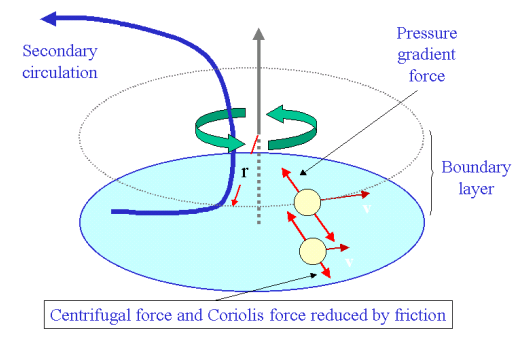
\includegraphics[width=2.4in]{gradient_wind2006B.png}}
	
	%	\noindent\includegraphics[width=20pc,angle=0]{H:/Documents/Admin/ESA/gradient_wind2006.png}
	\caption{a) gradient wind force balance in the primary circulation of a tropical cyclone b) disruption of gradient wind balance by friction in the boundary layer leaving a net inward pressure gradient that drives the secondary circulation with inflow in the boundary layer and outflow above it. Source: Smith, 2006}\label{fig:cyclone_circ}
\end{figure}

Surface friction in the boundary layer reduces the wind speed near the surface and therefore the centrifugal and Coriolis forces, but has little effect on the pressure field. There is therefore a new inward force in the boundary layer, driving inflow and the secondary circulation. The conservation of angular momentum means is objects will spin faster as they move toward the centre of circulation, so air increases its speed as it heads toward the centre of the tropical cyclone.


\subsubsection{Potential intensity}

To a good approximation, the secondary circulation in a tropical cyclone is a natural realisation of a Carnot heat engine, except that the engine does no work on its environment, the available work is locally dissipated and a fraction of the dissipated energy is recycled into the engine. A Carnot heat engine is the most efficient heat engine cycle allowed by physical laws. The Carnot perspective provides an upper bound on the maximum wind speed that a storm can attain.

\begin{figure}[h]
	\centering
	\noindent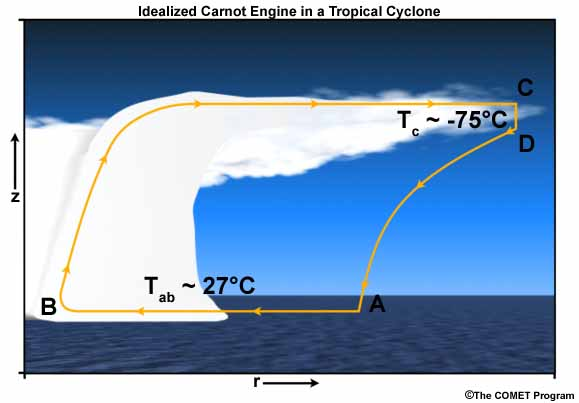
\includegraphics[width=20pc,angle=0]{carnot1.jpg}
	\caption{The Carnot cycle in a tropical cyclone. A-B: isothermal inflow of near-surface air; B-C: moist adiabatic ascent in the eye wall and outflow just below the tropopause; C-D: sinking of cooled air in the environment far from the tropical cyclone center. To close the system, D-A: the cooled air is assumed to return to the tropical cyclone environment adiabatically. Source:\cite{goescarnot}}\label{fig:cyclone_carnot}
\end{figure}

%CISK / WISHE
%\cite{emanuel1991theory} ref for carnot cycle
%vortical hot tower

%As this air ascends, 90\% of the stored energy is released by condensation, giving rise to the towering cumulus clouds and rain. The release of heat energy warms the air locally, causing a further decrease in pressure aloft. Consequently, air rises faster to fill this area of low pressure, and more warm, moist air is drawn off the sea, feeding further energy to the system. Thus, a self-sustaining heat engine is created.
%As little as 3\% of the heat energy may be converted into mechanical energy of the circulating winds. This relatively small amount of mechanical energy equates to a power supply of 1.5x1012 Watts - equivalent to about half the world-wide electrical generating capacity!
%http://www.metoffice.gov.uk/weather/tropicalcyclone/facts
%Emanuel theory 
%static vs dynamic theory

%In the northern hemisphere, positive vorticity at low levels and negative at upper levels. Vorticity decays with height. 

%It is the thunderstorm activity which allows the heat stored in the ocean waters to be liberated for the tropical cyclone development. (deep surface layer of conditional instability) - see Tory

%Intensification and decay
%Large vertical shear can weaken or destroy the tropical cyclone by interfering with the organization of deep convection around the cyclone center.
%(noaa website)
%maturity

%gray, frank montgomery, smith, tory book chapter- number of environmental conditions require to be satisfied for tc genesis.
%Emanuel
%ventilation
%Warm core is in thermal wind balance with the primary circulation.


\subsection{Steering of tropical storms} \label{steer}



%rotating winds of a tropical cyclone, combined with the north–south variation in the Coriolis parameter, induce relative vorticity asymmetries in the tropical cyclone (Fig. 8.60). These asymmetries are called the β–gyres.
%Tropical cyclones move in relation to the integrated, deep-layer (to \textasciitilde 17 km) environment flow in which they are embedded \citep{neumann1985role}.
% annulus degrees = see Carr 
%The motion of a tropical cyclone is highly correlated with latitude \citep{neumann1985role}. 
%5Chan 1985. (ref atm and ocean control sections). Low latitude easterlies and high lat westerlies, subtropical high.

A tropical cyclone is approximately 500-1000 km wide and 10-16 km high, set in much larger scale flow, so it can be treated as a solid object floating in the atmosphere \citep{chan2005physics}. Environmental steering is typically defined as the wind within an annulus centred on the tropical cyclone. e.g. 5-7 degrees (\citep{chan1982tropical}, \citep{chan1985identification} or 3 degrees (Franklin 1996). To define the steering flow, tropospheric layer means are better than single-level analyses \citep{velden1991basic}, with the deep layer mean (DLM)(1000-100 hPa) or mid-tropospheric level (500-700 hPa) often used. The vector quantity for the difference between the environmental steering and tropical cyclone motion is termed 'propagation' \citep{carr1990observational}. This difference arises from variations in the Coriolis parameter and environmental vorticity across the tropical cyclone. 

Depending on direction of movement of the storm, there is a different relationship with the surrounding flow \citep{chan1985identification}. Westward moving TCs move faster and to the left of the steering in the Northern Hemisphere, and eastward moving TCs move slower and to the right \citep{carr1990observational}.
%Importance of zonal direction of cyclone translation in determining the relationship between the environmental flow and cyclone movement. 

%Steered by surrounding flow and modified by Coriolis force (beta effect) and the horizontal vorticity gradient of the surrounding flow (chan physics review).
%NH Tcs move 10-20 degrees to the left and faster by 1ms than mid-tropospheric (700, 600, 500) at 6 degrees. 
%The beta effect - the cyclone and environment interact to modify the basic flow, and the vortex is then steered by this modified flow.

Studies have shown that depth of the steering layer is related to the strength of the cyclone \citep{velden1991basic}. For a more intense storm, there is greater vertical development of the cyclonic vortex, which is then advected by an environmental flow of greater depth. 

Tropical cyclone translation after landfall is affected by terrain, circulation environment, steering flow, TC intensity and structure among others \citep{xiao2013analysis}.
% effects of land, e.g. Philippines, Taiwan. track variation - interaction with topography (Wu and Kuo 1999), Taiwan


%Previous investigation into the sudden change in tropical cyclone track in four storms in the WNP suggested that such changes occurred near the centre of the MJO-scale cyclonic circulation or at the birfurcation of steering flows at 700 hPa \citep{wu2011observational}.

%Tropical cyclones forming between 5 and 30 degrees North latitude typically move toward the west. Sometimes the winds in the middle and upper levels of the atmosphere change and steer the cyclone toward the north and northwest. When tropical cyclones reach latitudes near 30 degrees North, they often move northeast

%Kim et al MJO effect
%Monsoon trough effect


\section{Impact of tropical storms}

Tropical cyclones are the most devastating natural hazards, affecting large populations in both the developed and developing world. Most of the damage occurs when tropical cyclones make landfall, and it is not only the destructive force of the strong winds, but also heavy precipitation and storm surge that cause widespread damage to communities.

Storm surges are responsible for much of the damage associated with landfalling tropical cyclones \citep{lin2012physically}. Storm surge is complicated, determined by the characteristics of the storms as well as shape and bathymetry of the coast, and the importance of the storm characteristics whilst over the open ocean and before landfall are also important. Rainfall distribution and intensity is complicated and depends on interactions on a variety of scales, with track, intensity, topography and environmental vertical shear all having an impact. Tropical storm wind fields change drastically when they make landfall, involving a complex interaction with the system and the underlying surface. The maximum damage of a tropical cyclone is not always at the point of landfall, but can be when it is further inland, for example when heavy rainstorms caused by interaction with mid-and lower-latitude systems once the storm is overland occur \citep{xiao2013analysis}. Although most damage occurs when tropical storms make landfall, they can also cause significant damage whilst at sea, mainly to the offshore industry. Loading on offshore structures is a complex function of not only characteristics of the wind field but also ocean characteristics including currents and waves \citep{done2014future}. Tropical-cyclone-wind resistant turbines have been deployed off the coast of China \citep{clark2014global}, to increase resilience to any future storms.

A recent notable tropical storm in the Western North Pacific is Super Typhoon Haiyan (2013). This is one of the most powerful typhoons ever to make landfall, with maximum sustained winds of 170 knots (88 m/s, 195 mph). Haiyan tracked over the Philippines archipelago, with storm surge primarily responsible for 6,300 dead, 1061 missing and almost 30,000 injured \citep{lagmay2015devastating}. %Average 472 fatalities a year (1983-2006) \citep{zhang2009tropical} 

Such landfalling typhoons also have a significant economic impact, for example Super Typhoon Herb (1996) caused 73.26 billion yuans  (£8.31 billion) in direct economic losses and became the costliest landfalling tropical cyclone in China at the time \citep{zhang2009tropical}. In China, there is an upward trend in the economic cost of landfalling tropical cyclones, and this is principally caused by economic development \citep{zhang2009tropical}.

%http://www.air-worldwide.com/Press-Releases/AIR-Estimates-Insured-Losses-from-Super-Typhoon-Haiyan-at-Between--USD-300-Million-and-USD-700-Million/

% From zhang2009tropical: In an average year, landfalling tropical cyclones cause 472 deaths and 28.7 billion yuans (2006 RMB) in direct economic losses, accounting for 0.38% of the annual total gross domestic product (GDP) of China. As the deadliest landfalling tropical cyclone, Super Typhoon Fred killed 1,126 people in 1994, making it the deadliest year (1,815 deaths). The costliest landfalling tropical cyclone was Super Typhoon Herb, which caused 73.3 billion yuans (2006 RMB) in direct economic losses in 1996, making it the costliest year (107.9 billion yuans). The direct economic losses and casualties of a landfalling tropical cyclone tend to increase with the northward shift in landfall track.



%%%%%%%%%%%%%%%%%%%%%%%%%%%%%%%%%%%%%%%%%%%%%%%%%%%%%%%%%%%%%%%%%%%%%%%%%%%%%%%%%%%%%%%%%%%%%%%%%%%%%%%%
\section{Tropical storm activity}

The Saffir-Simpson Hurricane Scale \citep{simpson1974hurricane} is often used to categorise tropical storms by intensity. Storms with maximum sustained winds of 38 mph (61 km/h, 33 knots) or less are called 'tropical depressions' and once over this threshold, are called 'tropical storms'. In the West Pacific basin, if maximum sustained winds reach 64 knots (33 m/s, 74 mph) the term 'typhoon' is used, and a 'Super Typhoon' is if the maximum sustained winds are at least 130 knots (67 m/s, 150 mph). %(http://www.srh.noaa.gov/jetstream/tropics/tc\_classification.html)
%(I need to remember if 1-min or 10-min. Which is US? Which is WMO?)

\subsection{Influence of the ocean} \label{ocean}

The ocean provides a source of energy to the tropical cyclone system by air-sea sensible and latent heat fluxes, determined by the sea surface temperature (SST). Many studies have shown that the SST must exceed 26$^{\circ}$C for tropical cyclones to form \citep[e.g.][]{palmen1948formation}. However, there is much research into this threshold \citep[e.g.][]{dare2011threshold, mctaggart2015revisiting}, highlighting basin-dependence and the importance of ocean temperature below the sea surface. The WNP has high SST throughout the year (\textgreater 28.5$^{\circ}$C) \citep{chan2007interannual}, relative to the suggested 26.5$^{\circ}$C threshold for genesis (section 1.2.1). Variability in activity is related to the SST pattern, with warm anomalies favouring intensification. The West Pacific is warm, past threshold limit, threshold more suitable for the North Atlantic, where more marginal.

The potential intensity of a tropical cyclone is directly related to the SST below the cyclone, all else being equal \citep{emanuel1991theory, holland1997maximum}, with higher SST promoting increased intensity. At high wind speeds, the surface wind stress generates strong turbulent mixing within the ocean. This causes entrainment of cooler water towards the surface from the thermocline and deepens the mixed layer.  The cooling of the SST is determined by the initial state of ocean, storm intensity, translation speed and storm size, and limits storm intensification, especially for slow moving storms, where SST cools more \citep{bender1993numerical, bender2000real}. During the lifetime of a storm, the wake produced can change considerably, for example Megi (2010) created a wake of 1.6$^{\circ}$C whilst in the Philippine Sea, but once in the South China Sea, cooling increased greatly to 7$^{\circ}$C \citep{d2014impact}. Due to this turbulent entrainment of cold water into the oceanic mixed layer induced by the TC, the state of ocean below the surface is also important to the cyclone system \citep{bender2000real, shay2000effects}.
%(see if any emanuel refs here - environmental control on...)
%Price 1981 - cooling 1 to 6C. \citep{price1981upper}
%Using satellites, observations of this cooling has been possible, 
%Cold wake of ~6C \citep{prasad2007upper}. 
%check Bender2000real.
%SST decrease induced by passage of a TC is approximately 1-6$^{\circ}$C  \citep{price1981upper}. 

The ocean heat content (OHC) in Joules (J) is a measure of the heat content within the ocean between two reference levels. 

\begin{equation}
OHC = c_{p} \int_{z1}^{z0} (T-T_{ref}) \rho dz
\end{equation} 	
%https://www.sharelatex.com/learn/Mathematical_expressions

%\begin{equation}
%$\displaystyle OHC = c_{p} \int_{z1}^{z0} (T-T_{ref}) \rho dz$
%\end{equation} 	

Tropical cyclone heat potential (TCHP) is vertically integrated heat content from the sea surface down to the 26$^0$C isotherm, which as at depth 'D26'.
% cannot find ref: as Gray (1968, 1978) suggested that depth of 60m is necessary for intensification.
%When this heat content is from the surface down to the 26$^0$C isotherm, it is termed tropical cyclone heat potential %(TCHP).
%Increased availability of sub-surface ocean observations, e.g. ARGO floats, since ...
%The ocean is the source of energy for a TC's intensification, typically down to 100-200m is important (Emanuel 1999) \citep{bender2000real}, \citep{shay2000effects}.
%Although WPAC SST is warm (generally above xyz), anomalously warm water can favour intensification. 

If the ocean warm layer (D26) is relatively shallow, (e.g. 60m) a positive SST anomaly is critical to intensification because the features can effectively deepen the warm layer and restrict the TC-induced cooling. If this layer is deep, e.g.\textgreater 105m, a warm feature is not required as the background is already sufficient to overcome the negative cooling feedback \citep{lin2008upper}.
%But isnt the warm SST anomaly needed in the first place?

In the WNP, intensification to category 5 needs SST around 29$^0$C and subsurface heat content required depends on the storm translation speed \citep{lin2009upper}. A shallow warm subsurface (D26 \textasciitilde 60m) is sufficient to intensify to a category 5 in a fast moving storm, but for slow moving storms, a much deeper warm layer is required \citep{lin2009upper}.

%Rapidly moving storms with deep oceanic mixed layer, SST feedback is of minor importance \citep{schade1999ocean}. All hurricanes attain their maximum intensity over warm ocean waters (does this mean the warmest or just above a threshold??) - from Prasad, referencing Goni and Trinanes, 2003

Typhoon Imbudo (2003) intensified from 56 knots (29 m/s, 65 mph) to 113 knots (58 m/s, 130 mph) in 12 hours when it passed over a region that increased TCHP by 100 kJ/cm$^2$. As the typhoon passed over these waters, the SST decreased by 3-4$^0$C alongside TCHP, but there was sufficient energy to negate the negative feedback of upwelling of cooler waters \citep{goni2003ocean}.
%But still there was cooling?


%On a much smaller scale, breaking waves and sea spray produced by TCs may change the wind stress \citep{moon2004effect}. Surface waves are a source of surface friction, moisture flux and ocean mixing and are a non-linear function of fetch and wind speed.

%Breivik et al. (2015) recently have demonstrated substantial improvement in climatological ocean biases with explicit treatment of surface waves. Waves generated by tropical cyclones are an important cause of infrastructure damage so an explicit and coupled treatment is desirable.

%%%%%%%%%%%%%%%%%%%%%%%%%%%%%%%%%%%%%%%%%%%%%%%%%%%%%%%%%%%%%%%%%%%%%%%


\subsection{Influence of the atmosphere}
%The atmosphere can maintain the TC or destroy it, principally through vertical wind shear.
A cyclone exists throughout the depth of the troposphere and so the atmospheric conditions have a large effect on the phenomenon. It has been established that vertical wind shear is detrimental to tropical cyclone genesis and intensification \citep[e.g.][]{chan1982tropical, McBride1995}, although mature, large tropical storms may resist relatively large wind shear \citep{zeng2007environmental}.

%One hypothesized pathway by which vertical shear affects tropical cyclones is mid-level ventilation, or the flux of low-entropy air into the centre of the tropical cyclone \citep{McBride1995}. Tropical upper tropospheric trough (TUTT) cells from the mid-latitudes can weaken tropical cyclones by introduction of vertical wind shear, but also bring a cyclonic PV anomaly, which may contribute to intensification \citep{zeng2007environmental}.
%EXPLAIN
%Strong vertical wind shear prohibits rapid intensification and most likely results in the weakening of TCs \citep{zeng2007environmental}.
%and a threshold of 12.5 ms$^-1$ above which TCs cannot form in the WPAC has been suggested \citep{zehr1992tropical}-seems to be a thesis - check this ref
%e and Zehr 1991, Zehr 1992 - thesis?)
%check zeng paper
% McBride and Tang for ventilation

The translation of TCs is largely determined by the large-scale atmospheric pattern, with mid-tropospheric levels (500 and 700 hPa) found to have the best correlation with TC direction and speed \citep{chan1982tropical} (\ref{steer}). If the passage of the storm is too slow, the cooling induced by the storm will inhibit intensification, and if it is moving too fast, the resulting asymmetric structure will also inhibit intensification \citep{zeng2007environmental}. Rapid intensification (RI) is An increase in the maximum sustained winds of a tropical cyclone of at least 30 kt in a 24-h period (\citep{nhc_gloss}). and for this to occur, a translation speed between 3-8 m/s is required. % (REF). % ref missing here

Although wind is the primary atmospheric control on TC activity, relative humidity and vorticity are also important.

% Fast translation speed and strong vertical shear and detrimental to TC intensification \citep{zeng2007environmental} and

%%%%%%%%%%%%%%%%%%%%%%%%%%%%%%%%%%%%%%%%%%%%%%%%%%%%%%%%%%%%%%%%%%%%%%%
\subsection{Tropical storm variability in the West Pacific}

Changes in atmospheric and oceanic conditions drive tropical cyclone variability. Tropical cyclone activity in most ocean basins including the WNP has a strong interannual signal \citep{landsea2000climate}, with variability observed in genesis location, track, intensity, landfall and lifetime.% (could use zhan2011contributions).

%Regions preferable for genesis. Or something like, genesis location is important and atmospheric conditions to maintain or dissipate storms are important. Distribution of SST important, also ocean at depth is important.

%(At the end mention interdecadal seasonal variability)

\subsubsection{El Ni\~{n}o}

It has been long established that the El Ni\~{n}o-Southern Oscillation (ENSO) (figure \ref{fig:nino}) is the principal driver of interannual variability in the Tropics. This phenomenon also has a marked effect on tropical storm activity in all basins. In a warm El Ni\~{n}o year, when the SST in the central and eastern equatorial Pacific is anomalously warm, there is a zonal displacement of annual mean tropical storm genesis location eastward \citep{lander1994exploratory, zhan2011contributions}. These storms tend to have a longer lifetime and can reach higher intensities before they recurve or meet land \citep{camargo2007cluster, chan1998seasonal}. In contrast, during La Ni\~{n}a years, the main region of genesis shifts westwards, with fewer intense storms.
%El Nino -weakening of Walker circulation. La Nina - strengthening.
%, Chan 2000, Wang and Chan 2002, for zonal displacement ENSO.


\begin{figure}[h]
	\centering
	\noindent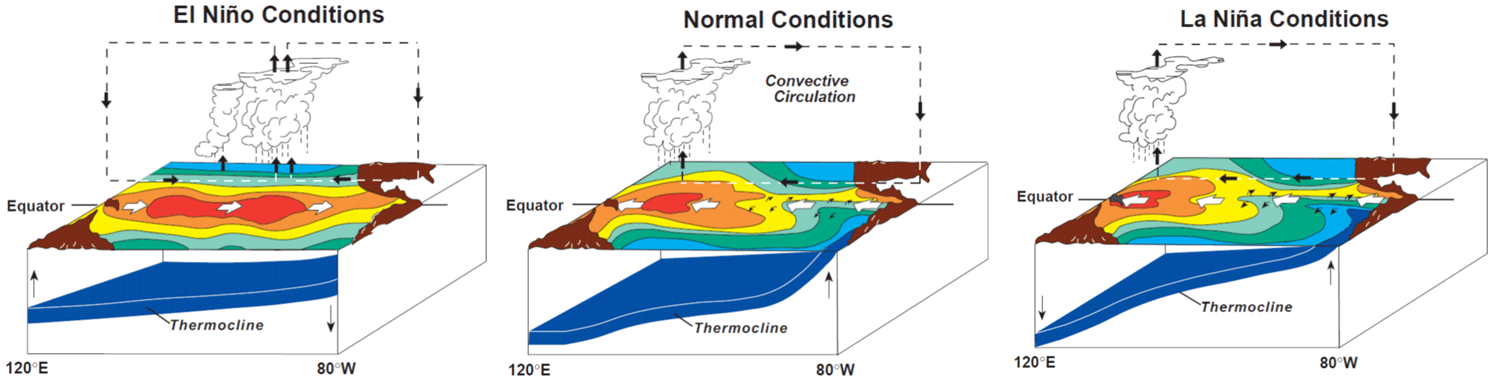
\includegraphics[width=40pc,angle=0]{Stressors_ENSO3.png}
	\caption{El Ni\~{n}o, normal and La Ni\~{n}a conditions in the atmosphere and ocean in the tropical Pacific. Source: \cite{noaa_enso}}\label{fig:nino}
\end{figure}


There is a significant difference in landfall location between El Ni\~{n}o and La Ni\~{n}a years. During El Ni\~{n}o, with more storms generated in the southeast quadrant of the WNP, they tend to recurve before landfall and affect Japan and Korea, with fewer across the Philippines and South China Sea \citep{liu2008interdecadal}. Whereas in La Ni\~{n}a years, the storms generate further westwards and are straight moving, with increased landfalls observed in China \citep{camargo2007cluster}.
%Does that mean that cyclones hitting China are weaker?

%ENSO affects the distribution of tropical storm numbers within the season \citep{lander1994exploratory}, as well as the landfall statistics, with \cite{yonekura2011statistical} finding significantly higher landfall rates in all coastal regions in La Ni\~{n}a.

%%%% MAKE FIGURE %%%%
% 	\begin{figure}[h]
% 		\noindent\includegraphics[width=20pc,angle=0]{Y:/Code_Data/Plots_NCAR/MAM/Maps/regions.png}
% 		\caption{Tropical storm tracks in 5 El Ni\~{n}o years and 5 La Ni\~{n}a years}\label{fregions}
% 	\end{figure}
% Look at Liu ZHou paper for years

Although El Ni\~{n}o has been shown to have a significant impact on tropical storm genesis location, the annual storm numbers have been shown to lack an ENSO signal \citep{lander1994exploratory}.

%ENSO - TC numbers: Chan 1985 too? Under debate - see zhan 2012.  However, El Ni\~{n}o has shown to have reduction in numbers - see Lander paper

%Wang and Chan (2002) observed an increase in the number of TCs in the WNP during strong El Ni\~{n}o events, though no significant linear relationship between TC number and indices of ENSO. A reduction in the number of TCs occurring in the summer following and El Ni\~{n}o has been found, related to Walker circulation (Chan 1985).

%The canonical eastern Pacific El Ni\~{n}o and the central Pacific El Ni\~{n}o have been shown to have different effect on TC activity in the Western Pacific (ref).

%In a study of intense typhoons, it was found that the interannual variations in the WNP were caused largely by changes in the planetary-scale atmospheric circulation and thermodynamic structure associated with El Ni\~{n}o \citep{chan2007interannual}.


\subsubsection{Other drivers of variability}

The Intertropical Convergence Zone, is the area encircling the earth near the equator where the northeast (N Hem) and southeast (S Hem) trade winds come together. Where the ITCZ is drawn into and merges with a monsoonal circulation, it is sometimes referred to as a monsoon trough. Most of the tropical cyclones that form in the WNP develop in the monsoon trough (MT) \citep{lander1994exploratory} and its location exhibits primary control on the distribution of TCs in the WNP \citep{wuinfluence}. 

\begin{figure}[h]
	\centering
	\noindent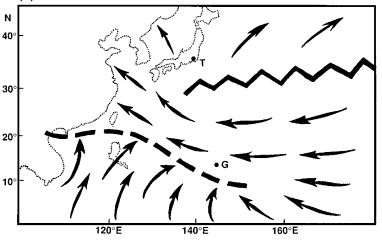
\includegraphics[width=20pc,angle=0]{MT_Lander.png}
	\caption{Long-term average of the low-level circulation during the summer in the Tropics of the western North Pacific. Bold zig-zag lines indicate ridge axes, and the bold dashed line indicates the axis of the monsoon trough. Arrows indicate wind direction. The locations of Guam (G) and Tokyo (T) are indicated. Source: \cite{lander1996specific}}\label{fig:MT}
\end{figure}

% when does the MT vary?
The monsoon trough is a climatological feature of low pressure and convergence (figure \ref{fig:MT}), with increased vorticity and it exhibits substantial migrations and changes of shape \citep{lander1996specific}. When the monsoon trough is defined as the contiguous region where long-term (1988-2010) mean July-November 850 hPa relative vorticity is positive, 73\% of all July-November tropical cyclones form within the monsoon trough \citep{molinari2013percentage}. This percentage displays interannual variation correlated with Ni\~{n}o 3.4 index, with more TCs forming in the MT in an El Ni\~{n}o phase \citep{molinari2013percentage}. The shift in genesis with ENSO phase has been related to the eastward extension of the monsoon trough and westerlies (associated with the increased cyclonic low-level vorticity) and the reduction in vertical wind shear near the date line \citep{lander1994exploratory, lander1996specific, wang2002strong}.
%See Camargo funny summary paper.
%Atmosphere - monsoon trough and subtropical ridge are important.See Harr and Elsbery 1991, 1995, Lander 1994, 1996, Liu and Chan 2002.

The Madden-Julian Oscillation (MJO) is a tropical mode of variability that has an intraseasonal time scale (30-90 days). It is characterised by an eastward progression of large regions of both enhanced and suppressed tropical rainfall, observed mainly over the Indian and Pacific Ocean. Over the western North Pacific (WNP), tropical cyclone activity appears to be strong when MJO related convection centre is in the WNP \citep{kim2008systematic}, however, no significant relationship with intensity has been found \citep{liebmann1994relationship}. As well as affecting the preferable region for genesis, TC tracks respond to the large-scale steering flows related to the MJO. When convection is in the equatorial Indian Ocean, tracks migrate eastward and when over the tropical WNP, they migrate westward \citep{kim2008systematic}.


%, Kim et al 1996.
%correct? See paper: Schreck et al (2012) 80-95\% WPAC TCs form in direct association with active MJO and/or active regions of various equatorial waves. 

%Studies have shown that the westerly phase of the Quasi Biennial Oscillation (QBO) corresponds to a larger number of TCs (refs) due to a decrease in the upper-tropospheric vertical shear over the tropics during the boreal summer. But does not hold during El Ni\~{n}o (See Chan 1995).

The subtropical high and mid-tropospheric flow pattern are important to TC movement \citep{chan1982tropical}. The strength and extend of the subtropical high influence where a TC will recurve (\ref{fig:STH}). %(ref steering section). How changeable is the sth?

\begin{figure}[h]
	\centering
	\noindent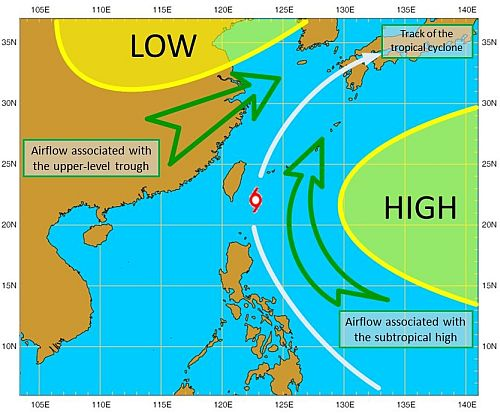
\includegraphics[width=16pc,angle=0]{typhoon16_1e.jpg}
	\caption{Subtropical High influence on TC movement. Source: }\label{fig:STH}
\end{figure}
%source http://www.weather.gov.hk/education/edu01met/01met_tropical_cyclones/ele_typhoon16_e.html

The Pacific Decadal Oscillation (PDO) exhibits variations in North Pacific SST over a decadal (20-30 years) timescale. It is similar to ENSO, with positive and negative SST anomalies, although it is on a much longer time scale and the most pronounced variations are at high latitudes, rather than in the Tropics  (figure \ref{fig:PDO}). The PDO Index is defined as the leading principal component of North Pacific monthly sea surface temperature variability (poleward of 20N for the 1900-93 period) (http://research.jisao.washington.edu/pdo/). The PDO has a significant impact on the subtropical high and mid-level steering during the peak TC season. It creates a north-south dipole of geopotential height over the WNP, affecting the subtropical high extension and intensity as well as the zonal winds \citep{liu2008interdecadal}.
%Check out Ho et al 2004 for PDO.
%NB wind stress changes with changing SST


\begin{figure}[h]
	\centering
	\noindent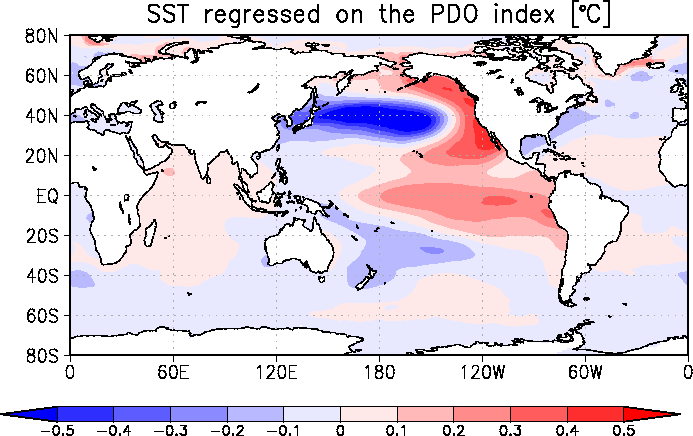
\includegraphics[width=20pc,angle=0]{pdo_pattern.png}
	\caption{Pacific Decadal Oscillation (PDO) positive phase. Figure from ADD SOURCE }\label{fig:PDO}
\end{figure}
%Add source to above: http://ds.data.jma.go.jp/tcc/tcc/products/elnino/decadal/pdo_doc.html


%WPSH is highly predictable and this can be used for tropical storm predictions \citep{wang2013subtropical}.

%Modes of variability - see Zhan 2012 review.
%Steering - Harr and Elsberry - straight, recurving, recurving north.
%IOD
%The intensity of a given storm depends on its surrounding environment.
%wang2013subtropical - Indian Ocean refs.

%Know about tropical waves - see Lu seasonal paper.

%IO importance - on MT?

Natural climate variability strongly modulates the seasonal statistics of tropical cyclones. 

%Affect of cyclone beforehand - upwelling is negative, but wave train is positive? (See camargo1)
%No - do not need to cover everything about TCs. Be specific and relevant.
%Something about historic activity can be divided into clusters, for example Camargo, Chan.

\subsubsection{Long-term variability}

Warming of the climate system is unequivocal \citep{stocker2013ipccb}, and as the internal energy available to weather systems such as tropical cyclones changes, activity of these phenomena is also expected to change. Warming of the ocean accounts for 93\% of the increase in the Earth's energy between 1971-2010, with 64\% of this in the upper ocean (0-700 m) \citep{rhein2013chapter}.

Modelling studies have consistently projected that greenhouse warming is likely to cause increases in the global average intensity of tropical cyclones and related rainfall rates \citep[e.g.][]{hill2011impact, knutson2010tropical, elsner2008increasing, bender2010modeled}, but some suggest that this is still within the range of natural variability. Many studies have shown that with an increase in SST in the coming decades, tropical cyclones will have increasing wind speeds \citep{bender2010modeled, murakami2012future, webster2005changes, emanuel2005increasing, knutson2010tropical, elsner2008increasing}, with \cite{emanuel2005increasing} suggesting that for every increase in SST of 1$^{\circ}$C, peak wind speed would increase by 5\%. The assumption is that the dominant effect of increasing carbon dioxide on tropical cyclones is through an increase in tropical mean sea surface temperature \citep{zhao2013robust}. However, modelling studies show that both spatial patterns of sea surface temperature warming and higher atmospheric carbon dioxide affect tropical cyclones independent of global sea surface temperature warming. % (ref)
% refs for within range of variability.
%The observed warming of the tropics of around 0.5$^0$C over the past 4 to 5 decades \citep{wang2010climate}. Consensus that the amount of energy will be the same, but higher lats will be increasingly exposed? \cite{huang2015change} suggested a suppressive effect of subsurface oceans on TC intensity in a warming environment due to sharpening of the subsurface vertical temperature profile, and therefore stronger ocean coupling (cooling).

Alongside SST warming, the effect of global sea level rise has consequences for damage caused by tropical cyclones. Global sea level has risen 10 to 20cm over last 100 years \citep{solomon2007climate} and it is very likely that the rate of global mean sea level rise during the 21st century will exceed the rate observed during 1971-2010 \citep{church2013sea}, so tropical cyclone-induced storm surge will become increasingly damaging phenomena. The water-holding capacity of air is a function of temperature, approximately doubling with each 10$^{\circ}$C increase in the range -20 to +45$^{\circ}$C \citep{fowler1995potential}. Therefore, in a warmer climate, precipitation from tropical cyclones will likely be more intense.

%That this rclationship is translated into pre¢ipitation potential is •vidcnccd by satdlitc obscrvations rcported by St•phcns (1990), which show a comparablc non-lincar rclationship b•tw••n s•a-surface tcmpcraturc and prccipitablc watet in a vcrtical air column ovcr the o¢cans. \citep{fowler1995potential}

%A number of factors that a warmer climate will affect on the activity and impact of tropical cyclones.

%Does it matter than here talking about modelling studies, before have talked about TCs in GCMs?

\section{Observations of tropical storms}
The historic record of tropical storm activity is longest for the North Atlantic, where records start in 1851 \citep{landsea2004atlantic}. Over the following decades, there has been a significant change in the methodology used to record such storms. In the early period, the main method for identifying tropical cyclones was by records of landfalling storms or by records of ships at sea \citep{vecchi2008estimates}. Further back in time, there were fewer ships and shipping lanes as well as fewer people living in the tropical and subtropical coastal regions \citep{landsea2007counting}, therefore it was possible that many storms were unrecorded. Aircraft reconnaissance in the West Pacific began near the end of the second World War and ended in 1987 \citep{knapp2013pressure}, and since then tropical storms have been monitored primarily by satellite \citep{lander1994exploratory}. The need for increased aircraft reconnaissance is acknowledged throughout the research and operational communities, with a recommendation from the World Meteorological Organisation (WMO) to 'realize the goal of regular and coordinated aircraft reconnaissance in the western North Pacific and other TC basins' \citep{wmoitwc8}. As part of government-led research, Japanese researchers are planning to have aircraft reconnaissance in the WNP from 2017 to at least 2020 \citep{nhkhurricanehunter}.

%, as many tropical cyclones(remove?)  were likely undetected over the tropical ocean in the pre-satellite era \citep{camargo2007cluster}

It is well established that although records begin many decades ago for some basins, they are only really trusted since the satellite era, ie. around the 1970s \citep{landsea2007counting} when global observations were possible. The observed time series of WNP tropical cyclone activity appears to be affected by artefacts of the changing observing system  \citep{lander1994exploratory, knapp2013pressure}, including the increasing use of satellite data and refining these methods, e.g. the Dvorak technique.
% and procedural changes . \citep{schreck2014impact} \citep{knapp2010international}

There are a number of agencies that produce Best Track records of tropical storm activity. The  International Best Track Archive Climate Stewardship (IBTrACS)\citep{knapp2010international} database consists of data from the World Meteorological Organization (WMO) Regional Specialized Meteorological Centres (RSMC) and Tropical Cyclone Warning Centres (TCWC) \citep{knapp2010international}. In the West Pacific region, data from the following agencies is available:

\begin{itemize}
	\item Fiji Meteorological Service (as RSMC Nadi)
	\item Japan Meteorological Agency (JMA) (as RSMC Tokyo)
	\item China Meteorological Administration’s Shanghai Typhoon Institute (CMA/STI)
	\item Hong Kong Observatory (HKO)
	\item U.S. Department of Defense Joint Typhoon Warning Center (JTWC)
\end{itemize}

For the WPAC region, JTWC storm data is most widely used \citep{knapp2010international}. All of the other agencies in this list provide data for a specific region in the West Pacific, rather than covering the entire basin. In some cases the same storms are tracked by multiple agencies, large differences in intensity can be found. There are also differences in lifetime as agencies employ different procedures for deciding when the first and last track point are determined.

%Modelling studies are vital, to learn more about TCs in the current climate and also to explore potential changes in the future.
% (tracks generallyu ok?), Also differences in lifetime - keep recording when goes ET or moves out of area of interest? Landfall in China goes further in CMA dataset (Matthias, pers comm). Different tracks, intensities, lifetime. eg. differences if calculating ACE. (see zhan2016cfs) Historical pressure record is more consistent between agencies than wind reports \citep{knapp2013pressure}.


\section{Representation of tropical storms in models}

\subsection{Global climate models}

Current CMIP5 (Coupled Model Intercomparison Project 5) models assessed in the IPCC Fifth Assessment Report (AR5) have a finest horizontal resolution in the atmosphere of around 70km, but the average is about 200km \citep{climodaus}, an increase from the previous four versions of the report.
It is well established that the current generation of global climate models (GCMs) are of insufficient resolution to simulate tropical cyclones in detail due to their low resolution in comparison to the size of the storm core \citep{lin2012physically} and the complex nature of tropical cyclone structure, although enhanced computing capabilities and parametrisations have resulted in better representation of tropical cyclones \citep{zhao2009simulations, bengtsson2007may, walsh2007objectively}.

Modern GCMs are capable of producing structures that can be recognized as similar to tropical cyclones at resolutions as coarse as 100 km (Knutson et al. 2010), but without the details of the core \citep{mcdonald2005tropical}. There is a need for very high resolution in order to simulate realistic storm intensities, \citep{bender2010modeled, emanuel2008hurricanes} for example it has been suggested that 2 km or less is needed to represent important physical processes in the tropical cyclone eyewall \citep{gentry2010sensitivity}, with \cite{chen2007cblast} suggesting that a resolution of 1 km is required to resolve hurricane eye wall convection and wind maxima.
%  (not realistic for GCM? Talking about RCM?)


Resolution is important for simulating storm intensity, but less critical for simulating the annual number of tropical cyclones and their geographical distribution. \cite{zhao2009simulations} found that a model with a resolution in 20-100km range was able to simulate climatology and interannual variability of tropical storm frequency without realistic distribution of storm intensity. Similar results were found by \cite{strachan2013investigating}, with realistic interannual variability of storm occurrence requiring resolutions of 100 km or higher, but skill was basin dependent. Different models produce substantially different annual global tropical cyclone frequencies and geographical distributions due to model resolution and physical parametrisations \citep{zhao2013robust}. It has been found that there are larger differences in tropical cyclone distribution between models than in the same model at different resolutions, suggesting a greater influence of model specifics than resolution \citep{shaevitz2014characteristics}.
%60km, 25 km, 12 km (NWP size).


%\subsection{Regional models}

%Regional models can be run at higher resolution than global models due to the reduced area over which calculations are being made. Typical resolution is ... and can be embedded in GCMs or GCMs downscaled.


%\newpage


\section{Seasonal prediction of tropical storm activity} % changed this from chapter to section

\subsection{Tropical storm forecasting techniques} % prediction?

%Remember focussing on climate, not NWP

The atmosphere is a chaotic system and so determinisitic predictability of weather phenomena, for example, tropical cyclones, is limited, and on a seasonal time scale, impossible. However, rather than forecasting exact cyclone tracks and dates of occurrence, predictions are made for basin-wide activity over a seasonal period.
Seasonal predictability of the climate system stems from the slowly evolving lower boundary, e.g. ocean forcing. The balance between the oceanic forcing and effects of random chaotic weather therefore determine the level of seasonal skill over a region \citep{rowell1998assessing}, and On a seasonal scale, atmospheric potential predictability is highest over the tropical oceans, where SST has an important effect, and this can be predicted using dynamical or statistical models \citep{rowell1998assessing}.
Seasonal tropical storm predictions are developed using dynamical, statistical, or statistical-dynamical models, with forecasts typically made 3 months ahead, e.g. March for the start of the season in June, with updated in May or June. 

%The time scales of changes in the ocean are much slower than in the atmosphere and can provide a source of predictability (e.g. ENSO). 
%The climate exhibits non-linear behaviour on a range of time scales, which may limit the seasonal climate predictability \citep{zhan2012seasonal}.
%, Palmer 2006.

%\begin{figure}[h]
%	\centering
%	\noindent\includegraphics[width=30pc,angle=0]{H:/Documents/Admin/ESA/seasonalforecasts.png}
%	\caption{Seasonal forecasts from different agencies. Most recent hurricane forecasts from each of the forecasting centers. Limits for the activity levels correspond to the ones defined by NOAA. Source: \citep{seasonalhurr}}\label{fig:seasonalforecasts}
%\end{figure}


%\begin{figure}[h]
%	\centering
%	\noindent\includegraphics[width=16pc,angle=0]{H:/Documents/Admin/ESA/na_ts_forecast_sm11.png}
%	\caption{Met Office seasonal forecast for North Atlantic. Also Hurricanes and ACE plots. None for the West Pacific yet as lacking skill. http://www.metoffice.gov.uk/weather/tropicalcyclone/seasonal/northatlantic2016}\label{fig:seasonalforecasts2}
%\end{figure}


%Predictable to some extent on seasonal time scale, but with large uncertainties. 
%predictability of large-scale environment


\subsection{Dynamical modelling}

In climate models accurate representation of the ocean is vital for climate simulation, especially over long periods, as the ocean represents a dynamic thermal reservoir that exchanges energy with the atmosphere. Fully-coupled atmosphere-ocean models, where heat and transport are fully represented and interactive, provide the best opportunity to capture relationships at a variety of scales.  These global models are vital as they can capture teleconnections, which are important for seasonal prediction. However, these are run at too coarse a resolution to capture the intensity. Model intensities are often not used directly, and instead are compared to the model climatology, which is then adjusted to cover the full spectrum of intensities. In order to extract the storms, a tracking algorithm needs to be applied to the model output. There are various different methods, for example tracking vorticity or minimum pressure, and then further thresholds are applied to select only tropical storms (e.g. warm core). %Tracking algorithms are not the same - not the same output storms, but with increasing resolution are better. Horn et al - thresholds. Basin-wide storm activity, released MAM? update June?


The skill of seasonal forecast models is often found to be higher using an ensemble than any single deterministic run \citep[e.g.][]{vitart2006seasonal}, and ECMWF use this ensemble approach. Dynamic models are important to explore the future climate, as long as they have sufficient skill at simulating the present climate and future forcings.

Seasonal forecasts for WNP tropical cyclone activity from dynamical models are produced by the European Centre of Medium-range Weather Forecasting (ECMWF). They have produced operational seasonal tropical cyclone forecasts for all basins since 2001 with their global coupled model. Predictions include tropical storm frequency, typhoon frequency, track density and accumulated cyclone energy (ACE) \citep{zhan2012seasonal}.

% Ensembles better than deterministic - see molinari cfs paper

%IRI uses\ a two step approach, whereby first SSTs are predicted using statistical or dynamical models, then atmospheric models are forced with these \citep{camargo12007seasonal}. IRI issues ACE forecast. IRI are probabilistic, normal , above normal, below normal \citep{camargo12007seasonal}. In both cases, TCs then tracked.
%ECMWF resolution
%IRI hybrid?????? , and the International Research Institute for Climate and Society (IRI). 
%Importance of ocean and ENSO prediction (refer to enso section). ENSO on SST field, but also on atmospheric pattern. Seasonal prediction of tc landfall represents a major challenge for dynamical models \citep{camargo12007seasonal}.\\
%\citep{rowell1998assessing} GCM skill in potential predictability
%\citep{vitart2006seasonal}
%\citep{mcdonald2005tropical}
%\citep{shaevitz2014characteristics}

%Limits of dynamical models for seasonal forecasting:
% \begin{itemize}
%	\item Resolution insufficient to capture storm structure and intensity (BUT there can be regional or hi res global dynamical models too?)
%	\item Global teleconnections need to be represented (and are they not?)
%	\item Model biases are present, which need to be corrected for
%	\item Limitations of the tracking methodologies (only apply to dynamical models?)

%\end{itemize}


%What are plans for operational - future - higher res, ensembles, physics problems to solve
%Landfall forecasts
%Modes of variability are important - teleconnections, also processes in the cryosphere, land, stratosphere, ocean, need fully coupled global  model.
%GloSea5, ECMWF and local models.
%bogussing? 

%basin wide and lead time 

\subsection{Statistical models}  
It has long been established that large-scale variability affects tropical cyclone activity globally. If a robust relationship between large-scale predictors and this activity can be found, it is possible to make predictions about future activity using statistical analysis.

The first region over which a statistical forecast for tropical cyclone activity was produced was the Australian region, in the late 1970s and 1980s \citep{nicholls1979possible, nicholls1985predictability}, with forecasts for the North Atlantic starting in 1984 \citep{gray1984atlantic}.

The first operational tropical cyclone forecasts for the West Pacific were issued by the National Climate Center (NCC) or CMA (China Meteorological Agency) in 1994 but these were only available in China \citep{zhan2012seasonal}. NCC currently issue seasonal forecasts of WNP tropical cyclone activity in March, with updates in June. The predictors are ENSO index, 500 hPa geopotential height over the Pacific and Australian region, convective activity over the WNP, vertical wind shear of zonal wind over the WNP and tropical eastern Pacific prior to the season \citep{zhan2012seasonal}.% EPAC Matters?

In 1997, The City University of Hong Kong, China (CUHK) started to issue seasonal forecasts to the public.  This scheme used SST anomalies as a proxy for ENSO signal, the large-scale circulation over Asia and the western Pacific, and trend or climatology and persistence \citep{chan1998seasonal}. New predictors related to ENSO including changes to the Southern Oscillation, Australian monsoon and subtropical high in the South Pacific have since been identified \citep{cl2001improvements}.
%persistence?
%Also did landfall in South China and Korea and Japan in 2009 and 2010 - still going?
%What is the CSL scheme? Does it stand for something? Not mentioned in the paper in 1998 - this is the one that details the model first used in 1997.
%(CHUK forecast 1997 or check this - is it 2000) The CSL scheme proposed by Chan et al 1998 
%.Relationship with the southern hemisphere related to the La Ni\~{n}a cold event.
Previous work by \cite{lu2013seasonal} examined the seasonal predictability of tropical cyclones affecting Taiwan using an empirical model. They found some skill in predicting accumulated cyclone energy (ACE) in the peak season (JJAS) using the SST in three regions and the sea level pressure (SLP) over an area in East Asia as predictors. 


%based on scientific understanding of the oceanic and atmospheric influence on tropical cyclones.
%Talk about verifying model using same dataset and similar region over Taiwan. Extending region to include more landfalling storms.

%Alongside CUHK and NCC, Tropical Storm Risk (TSR) also issue a statistical forecast for the WNP.
%statistical forecasts from CityU, National Climate Center China (NCC), Tropical Storm Risk (TSR) for the WNP. 

%Using a multivariate linear regression procedure, some skill is found using 3 regions of sea surface temperature and one region of sea level pressure predictors in forecasting the ACE over Taiwan. 
%Usually issued in March or April, with update in June or July.
%Seasonal statistical model - predictability from the spring to summer evolution of the monsoon subtropical high-ENSO system in association with the evolution of the Indo-Pacific SST anomalies \citep{lu2013seasonal}.

%Statistical modelling section - can also use statistical models of the large-scale environment to predict storm intensity distribution \citep{lee2015probabilistic}.
%Estimating or predicting landfall is important. Can create genesis models, track models etc. all from large-scale environment.

Limitations of such statistical forecasts include the dependence on historic observed data. this data is relatively limited (50 years) and has associated biases and errors. They assume stationarity of relationships and are unable to be used for climate change projections.
%Need to have cross correlations. Climate projections are difficult as rely on the signal at present (and in historic record).

%Limitations of statistical models for seasonal forecasting:
%\begin{itemize}
%	\item Dependent on historic observed data (limited and short record)
%	\item Climate projections difficult as future projections rely on present signal
%	\item Often assumes stationarity in relationships

%\end{itemize}

Alongside statistical and dynamical approaches, hybrid statistical-dynamical approaches have increased in popularity in recent years.

\subsection{Hybrid dynamical-statistical models}  
These models are a combination of the dynamical and statistical modelling approaches. A statistical model is developed based on either observations or output from a climate model seasonal prediction, and then this is applied to the seasonal prediction using predictors from a dynamical model. Skill of this model depends on robustness of the statistical relationship as well as the skill of the model to predict the predictor. \cite{zhan2016cfsv2} showed that a hybrid dynamical-statistical model showed better skill at longer lead times that the pure statistical model at predicting seasonal accumulated cyclone energy (ACE).
%BUt this PHd will focus on statistical?
% stationarity

%Quick summary sentence about timing of the forecast.
%ENSO predictability follows a cycle, where state for 4-6 months can be relatively accurately predicted between July and November \citep{camargo12007seasonal}. Once an episode has begun, predicting its continuation for the next 9-12 months is much easier than predicting its initial appearance \citep{camargo12007seasonal}.

%Relate this to TC season and timing of forecasts.

%\subsubsection{Seasonal forecast verification}  

%Previous studies have created statistical models of ACE or other tropical storm diagnostics such as frequency etc. (eg. Chan, Lu), and here we add to this by including the sub-surface ocean state in terms of ocean heat content and tropical cyclone heat potential.ADD LANDFALL
%provides more information over the depth of the ocean, important for intensity of the storms (ref intro).

Most seasonal projections are basin-wide. Here, we explore seasonal forecasts for a specific region of landfall and utilise current reanalysis datasets, including data on the deeper ocean. We also extend the lead time of predictability into the previous 15 months before the season.%....... Lu at al did the Taiwan region 6 months in advance. Others have focussed on basin-wide forecasts. EXTEND

%%%%%%%%%%%%%%%%%%%%%%%%%%%%%%%%%%%%%%%%%%%%%%%%%%%%%%%%%%%%%%%%%%%%%%%%%%%%%%


%How does my work compare to what has already been done.



\section{Characteristics of extra-tropical cyclones}

%
%\section{Characteristics of extra-tropical cyclones}
Extra-tropical cyclones are a dominant feature of the mid-latitudes, associated with strong winds, precipitation and temperature changes. An extra-tropical cyclone is a low pressure system that primarily gets its energy from a horizontal temperature gradient. They have frontal features, i.e. they are associated with cold fronts, warm fronts, and occluded fronts and in the northern hemisphere have winds counter clockwise. Like tropical cyclones, they transport heat and moisture from the Tropics towards the poles and they are embedded in mid-latitude westerlies, travelling in an eastward direction.

%what kind of intensities? named?

\section {Formation and structure of extra-tropical cyclones}
%Formation of jet streams? - no, not jet streams
%
%\begin{figure}[h]
%	\centering
%	\noindent\includegraphics[width=20pc,angle=0]{H:/Documents/Admin/ESA/jetstream3.jpg}
%	\caption{North hemisphere cross section showing jet streams and tropopause elevations. Source: \cite{noaa_jetstream}}\label{fig:jetstream}
%\end{figure}

The first conceptualised model of the typical life-cycle of mid-latitude cyclones is the Norwegian model (e.g. Bjerknes and Solberg). This was proposed in the 1910s and 1920s and describes the evolution of a cyclone from an incipient frontal wave with cold and warm fronts, through intensification, maturity and decay (figure \ref {fig:norwegian_maps}).

\begin{figure} % remove [h] and this appeared in the correct place
	\subfloat[Initial state]{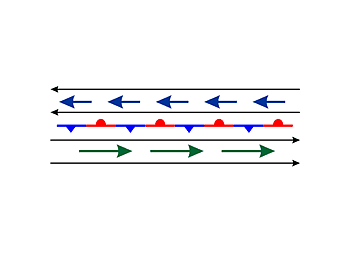
\includegraphics[width=2.0in]{cyclo1.png}}  % H:/Documents/Admin/ESA/Figures/
	\subfloat{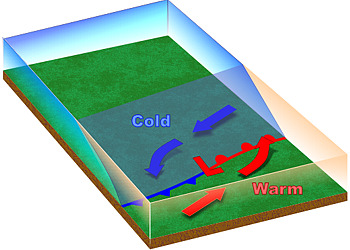
\includegraphics[width=2.0in]{wave23d.jpg}} 
	\subfloat[Beginning stage]{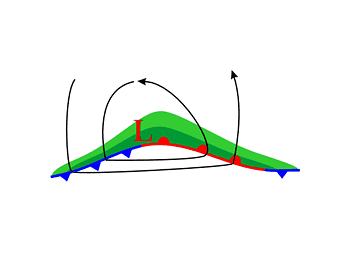
\includegraphics[width=2.0in]{cyclo2.png}} 
	\subfloat{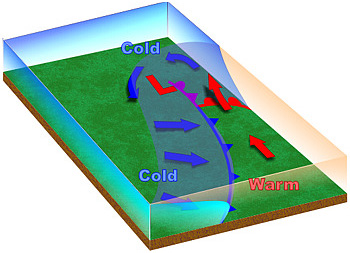
\includegraphics[width=2.0in]{wave43d.jpg}}  		
	\subfloat[Intensification]{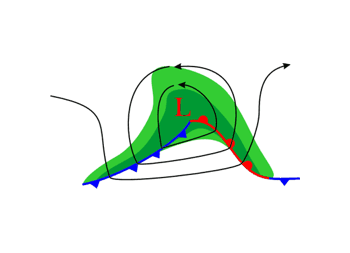
\includegraphics[width=2.0in]{cyclo3.png}} 
	\subfloat{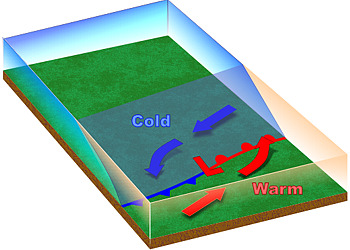
\includegraphics[width=2.0in]{wave23d.jpg}} 
	\subfloat[Mature stage]{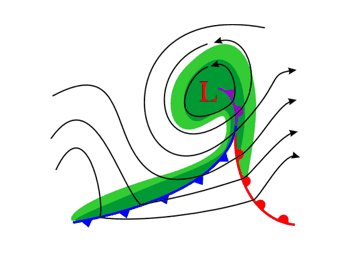
\includegraphics[width=2.0in]{cyclo4.png}} 
	\subfloat{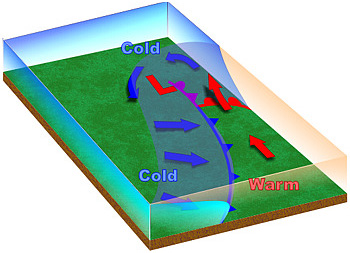
\includegraphics[width=2.0in]{wave43d.jpg}} 
	\subfloat[Dissipation]{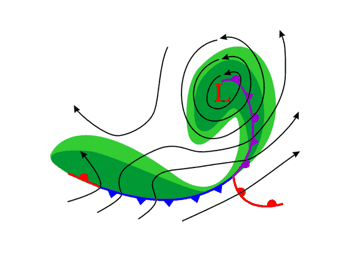
\includegraphics[width=2.0in]{cyclo5.png}} 
	\subfloat[]{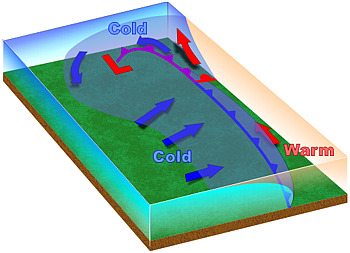
\includegraphics[width=2.0in]{wave53d.jpg}} 
	
	\caption{The Norwegian cyclone model in (1) map view (2) and 3-D view.  Source: \cite{norwegian}}\label{fig:norwegian_maps}
\end{figure}

One condition that favours cyclogenesis is a baroclinic zone, i.e. a region of large temperature change across a short horizontal distance near the surface, e.g. frontal zones. Above (near the tropopause) and parallel to this baroclinic zone is often a strong jet stream, driven by the thermal wind effect \ref{stull}. A wave develops on the front as an upper level low pressure system embedded in the jet stream moves over the front. As the air masses begin to rotate, defined cold and warm fronts develop. The wave intensifies and the low pressure centre deepens. The warm sector narrows as the cold front rotates around the cyclone faster than the warm front, and an occluded front develops where the cold front overtakes the warm front. As the cold front continues advancing on the warm front, the occlusion increases and eventually cuts off the supply of warm moist air, causing the low pressure system to gradually dissipate \citep{norwegian}. Precipitation occurs as air is forced to rise ahead of the warm front and the cold front. The more dense cold air undercuts the warm air and the less dense warm air rises above the cold air.

%http://weatherfaqs.org.uk/node/98
%As with the Norwegian cyclone model, the Shapiro-Keys model has an incipient cyclone develops cold and warm fronts, but in this case, the cold front moves roughly perpendicular to the warm front such that the fronts never meet, the so-called 'T-bone'. Also, a weakness appears along the poleward portion of the cold front near the low center, the so-called 'frontal fracture' and a back-bent front forms behind the low center. (In the final stage), colder air encircles warmer air near the low center, forming a warm seclusion. 

An alternative model is the Shapiro-Keyser model. The main difference from the Norwegian model is that the cold front moves roughly perpendicular to the warm front and they never meet. The occluded front is due to a weakness in the cold front near the low centre.
%The occluded front is an extension of the warm front rather than a result of the cold front catching up with the warm front. Both are valid and suited to different scenarios.. e.g....

%Conditions favourable to cyclogenesis are a baroclinic atmosphere (a region of large temperature change across a short horizontal distance near the surface), there is often an associated a strong jet stream running parallel at upper levels.
%what about mositure?
%cyclogenesis involves sea-level pressure decrease as the low pressure centre deepens, upward-motion increase, and vorticity increase.

Energy from baroclinicity in the atmosphere. This is in contrast to tropical cyclones, where there is little temperature contrast across them and they get their energy from the underlying ocean. Much like tropical cyclones, extra-tropical cyclones are moved by the jet stream and by other large-scale components of the global circulation \citep{stull}.

%Baroclinic instability is due to a horizontal temperature gradients in a rotating environment. 

%What season? winter storms or summer storms? extratropical transition?

%extratropical ocean-atmosphere interaction dominated by atmosphere forcing the ocean, but with variability with oceanic processes more important to SST in the vicinity of WBCs (smirnow).

%baroclinic wave, steering level. Steered by large scale, much like TCs?

Figure \ref{fig:ET_structure} shows a mature extra-tropical cyclone in more detail. An extra-tropical cyclone is typically larger than an average tropical storm, (approximately 1000 km)
As an extra-tropical cyclone moves eastwards, ahead of the warm front, there stratiform cloud as warm air is forced to rise and cool. Behind the warm front is the warm sector, of relatively warm air and generally clear skies. At the cold front, dense cool air undercuts the warm, moist air and forces it steeply upwards, with a band of cumuliform clouds, heavy rain and thunderstorms. Following the passage of the cold front, there is cooler air, bright skies and showers, and a marked veer in wind direction. The near surface winds converge towards the low pressure centre. Structurally, extra-tropical cyclones are 'cold-core', unlike tropical cyclones, which are 'warm core'.
%Cold sector surface flow is from the northwest
%Warm sector surface flow is from the southwest, bringing warm low-latidude air poleward and upward 'warm conveyor belt', associated with weak turbulent heat fluxes at the surface (warm path pahper?). Warm conveyor belt, cold conveyor belt, dry intrusion.

\begin{figure}[h]
	\centering
	\noindent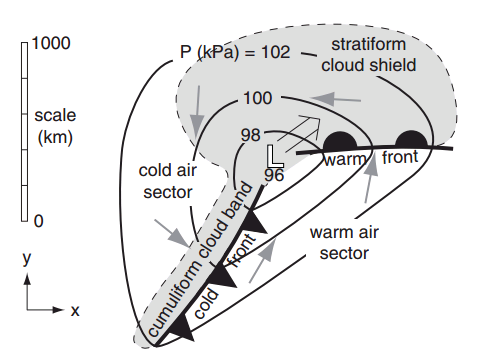
\includegraphics[width=20pc,angle=0]{ET_structure.png}
	\caption{Components of a typical extra-tropical cyclone in the N. Hemisphere. Light grey shows clouds, dark grey arrows are near-surface winds, thin black lines are isobars (kPa), thick black lines are fronts, and the double-shaft arrow shows movement of the low centre 'L'. Source: \cite{stull} }\label{fig:ET_structure}
\end{figure}


%\section {Impact of extra-tropical storms}

\subsection {Extra-tropical storm activity} %ocean, atmos, variability
%
Much like with tropical cyclones, the variability of extra-tropical storm activity is due to both atmospheric and ocean conditions. These storm systems extend through the atmosphere, however, underlying conditions in the MBL are important too. The marine boundary layer (MBL) is the part of the atmosphere that lies over the ocean surface and is directly influenced by it.  Variations in the ocean surface therefore affect the cyclone, affecting ocean-atmosphere exchanges of heat, moisture and momentum.

%Due to variations in the atmosphere and ocean - baroclinic atmosphere required for cyclogenesis (ref section). 

Extra-tropical storms are driven by strong temperature gradients (section 3.1) and in the North Atlantic, often develop in baroclinic zone over Gulf Stream. In the MABL, the Gulf Stream directly influences air temperature and pressure fields but also has effects throughout the entire troposphere, with upper-tropospheric divergence exhibiting a structure similar to the surface convergence and precipitation patterns, all meandering with the Gulf Stream (\citep{minobe2008influence}).
%Major storm tracks are organised along or just downstream of the main oceanic frontal zones (Nakamura et al 2004).
%Sheldon(The atmosphere above the Northern Hemisphere’s western boundary currents (the Gulf Stream and Kuroshio) are maximums in the winter atmospheric variability on a synoptic timescale of 2-6 days (Lau and Wallace, 1979; Blackmon, 1976; Hoskins and Valdes, 1990). These regions of synoptic variability are called the storm tracks and the variability is measuring the growth of extra-tropical cyclones that occur there (Dacre and Gray, 2009).)

In the marine atmospheric boundary layer (MABL), the Gulf Stream directly influences air temperature and pressure fields locally and also throughout entire troposphere, with upper-tropospheric divergence exhibiting a structure similar to the surface convergence and precipitation patterns, all meandering with the Gulf Stream (\cite{minobe2008influence}). Extra-tropical storms are driven by strong temperature gradients and in the North Atlantic, often develop in the baroclinic zone over Gulf Stream. Here, strong oceanic fronts that help to maintain the strong baroclinicity that is required to maintain them \citep{nakamura2004observed, nakamura2008importance, hoskins1990existence}

%\cite{nakamura2004observed}
%As the surface air temperature over the open ocean is linked to SST underneath, maritime surface baroclinic zones tend to be anchored along oceanic fontal zones [NS04]. Though acting as thermal damping for the evolution of individual  eddies, heat exchange with the underlying ocean, on longer time scales, can act to restore atmospheric near-surface baroclinicity against the relaxing effect by atmospheric eddy heat transport, as evident in sharp meridional contrasts in upward turbulent heat fluxes observed climatologically across midlatitude frontal zones [Oberhuber, 1988]. Some observations are shown in section 2 to suggest that SST anomalies in a midlatitude frontal zone can likely play a more active role in the air–sea interaction than act to damp  tmospheric anomalies thermally Hoskins and Valdes (1990) mean diabatic heatin as a result of the warm ocean current restores the meridional atmostpheric temperature gradient and therfore baroclinciiy, that is vital to the storm tracks existence.

%nakamura et al 2008 \cite{nakamura2008importance}
%and booth et al 2010 - air-sea heat exchanges at oceanic fronts restore the baroclinicity of the atmosphere at low levels.
%shear instability not parametrised in current generation of GCMs.

%GCMs generally simulate the storm tracks well (d'Andrea et al 1998)as they are large-scale phenomenon of the atmospheric circulation. Also climate models can capture the structure of ETCs (cite{\catto2010can}).
%Atmosphere-ocean interactions are their strongest over WBCs, e.g Gulf Stream. Strong fluxes of heat and moisture anchor the storm tracks to the WBCs (Nakamura et al 2004). allows for recurrent develpoment of storm tracks - creates baroclinicity?

%Deep ascent over the Gulf Stream is a result of extreme events, i.e. extra-tropical storms \citep{minobe2008influence}(check this)
%The storms occur in these locations as the strong oceanic fronts help maintain the surface baroclinicity required to produce them (Nakamura and Shimpo, 2004 Nakamura et al., 2008; Sampe et al., 2010).  (sheldon thesis).
%SHELDON THESIS:
%The Gulf Stream is the western boundary current for which the most links to deep convection have been found. %The deep ascent over the Gulf Stream found by Minobe et al. (2008) is a result of extreme events that skew the mean to ascent, and their results do not represent an average day in that region. The ascent above the Gulf Stream being a product of extreme events is consistent with the region also being the centre of action for winter synoptic systems in the Northern Hemisphere (Hoskins and Valdes, 1990).


\subsubsection {The Gulf Stream}

Global atmospheric circulation is characterised by easterly trade winds in the Tropics and the westerlies in the mid-latitudes.  The atmosphere exerts a force on the ocean below, which is also affected by the rotation of the earth, a factor which increases with proximity to the poles. Surface currents located on the western side of ocean basins are must faster than on the east and are among the fastest surface currents in the ocean (\citep{nasa_ocean}).  These currents also extend much deeper than most other surface currents, and are deflected by the continental margins, which prevent these currents from flowing onto the shallow continental shelves \citep{nasa_wbc}.
%Waters in western boundary currents (WBCs) typically move 40 to 120 km (25 and 75 mi) per day (\citep{nasa_wbc}). 
The Coriolis effect increases with latitude, and so is stronger in the latitudes of the westerlies than in the latitudes of the equatorial trade winds. Surface waters build up on the western side of ocean basins, resulting in the ocean-surface slope to be steeper on the western side (versus eastern side), which leads to a faster geostrophic flow on that side \citep{nasa_wbc}.

The Gulf Stream can be seen in Sea Surface Temperature data (SST), transporting a warm tongue of water poleward and eastward (figure \ref{fig:GS_map}). On the northern edge, there is a strong SST gradient while to the south, eddies tend to erode this gradient.

\begin{figure}[h]
	\centering
	\noindent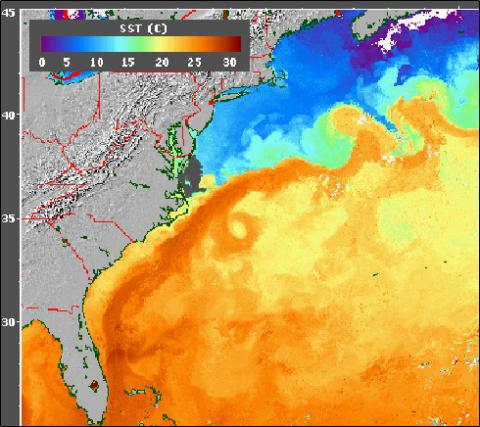
\includegraphics[width=14pc,angle=0]{GulfStream.jpg}\\ % H:/Documents/Admin/ESA/Figures/
	\caption{The Gulf Stream, revealed through SST data, made from the AVHRR (Advanced Very High Resolution Radiometer) sensor carried on a NOAA satellite. In this image, purple and blue represent the coldest temperatures (between 0-15 $^0$C) and orange and red represents the warmest temperatures (between 22-32 $^0$C). Source: \cite{gsnasa}}\label{fig:GS_map}
\end{figure}


%Deep ascent over the Gulf Stream is a result of extreme events, i.e. extra-tropical storms \citep{minobe2008influence}(check this)

It has been found that these extra-tropical storms occur in locations such as the Gulf Stream, where there are strong oceanic fronts that help to maintain the strong baroclinicity that is required to maintain them (Nakamura and Shimpo, 2004 Nakamura et al., 2008).
%The storms occur in these locations as the strong oceanic fronts help maintain the surface baroclinicity required to produce them (Nakamura and Shimpo, 2004 Nakamura et al., 2008; Sampe et al., 2010).  (sheldon thesis).

%heat from the tropics poleward - affects cyclogenesis (how is this related to temp?)


\subsection{The warm path}

Previous studies \cite{vanniere2017cold} \cite{sheldon2017warm} have suggested a new mechanism by which the SST distribution of the Gulf Stream impacts cyclones over the North Atlantic Ocean. The mechanism consists in an intensification, and possibly a destabilization, of the frontal circulation embedded in the cyclones. 

The 'warm path' is the mechanism of oceanic forcing  associated with impact of the Gulf Stream warm tongue on the warm sector of cyclones. Here there are weak air-sea heat fluxes, which is in sharp contrast to what occurs in their cold sector.

In \cite{sheldon2017warm} , this warm path mechanism has been examined using one case study on January 14th 2004, with a MetUM simulation (12km) integrated for 72 hours. A 'SMTH' experiment used a smoothed Gulf Stream warm tongue SST, a 'COOL' reduced the SST everywhere by 3K and the control used an unperturbed SST. Results showed that the Gulf Stream has a significant impact on the upward motion present in the cyclone, with back trajectories providing a useful tool. 

\begin{figure}
	
	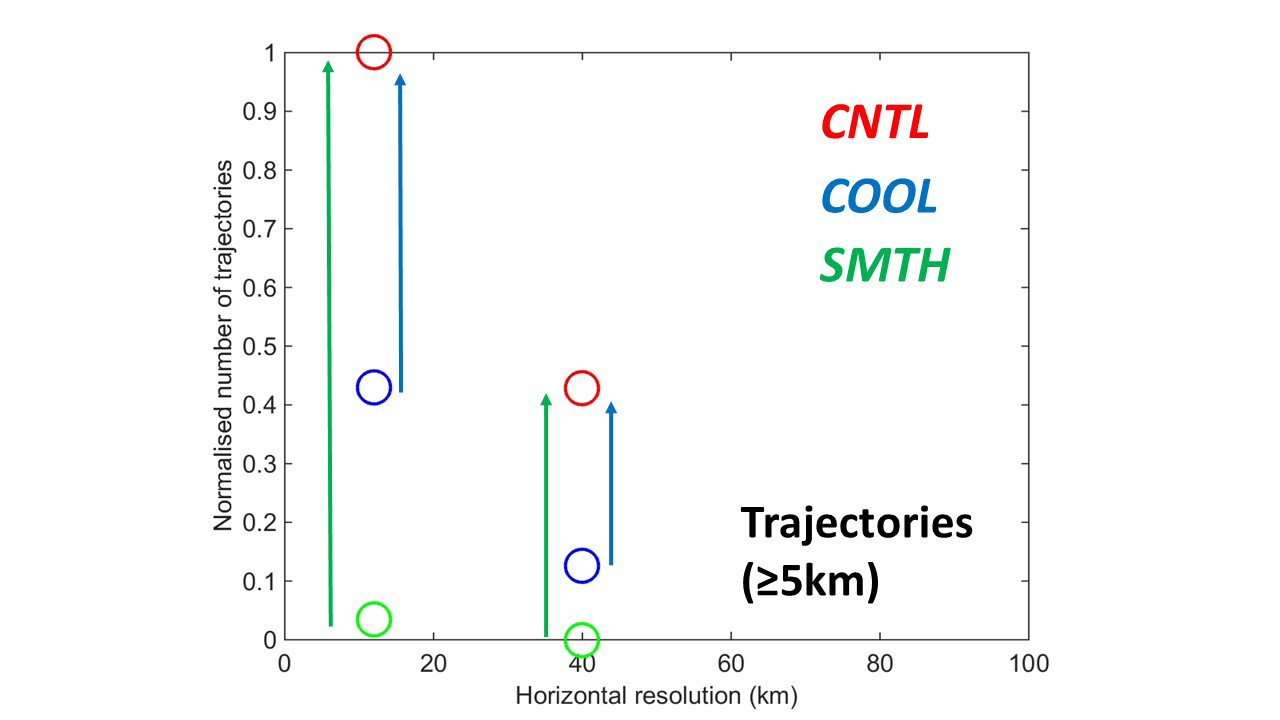
\includegraphics[width=22pc,angle=0]{warmpath_result.png} % H:/Documents/Admin/ESA/Figures/
	\caption{Number of back trajectories (circles) with heights z 5km at t=24h and reaching low levels over the ocean at t=0h: red for CNTL, blue for COOL and green for SMTH. The arrows indicate a measure of oceanic forcing when comparing CNTL,SMTH or CNTL,COOL. Normalized such that the number for CNTL at 12km resolution is unity. Source: Sheldon et al. 2016}\label{fig:wp_result}
	\centering
\end{figure}

Figure \ref{fig:wp_result} shows that at both model resolutions (12 km and 40 km), the control simulation has more than double the number of trajectories that the perturbed simulations, with the smooth simulation having a the fewest. Oceanic forcing is measured by the number of trajectories as this is related to upward mass transport, which scales with the diabatic heating (due to condensation of water vapour carried in the flow) in the ascending branch (Sheldon et al., 2016).

Thermodynamic and dynamic mechanisms have been proposed. For the thermodynamical mechanism, in the control experiment trajectories are parallel to the Gulf Stream, with no significant loss of heat and possible gain of moisture, maintaining high $\theta$e values. In the smooth simulation, air parcels cross SST contours, reducing $\theta$e and the likelihood of ascent. The dynamical considerations are that, due to stronger SST gradients in the control experiment, a thermally driven cell enhances the frontal circulation, increasing the feed into the warm conveyor belt. Also, it is possible that the stronger SST gradients destablise the frontal circulation by enhancing the vertical wind shear (Sheldon et al., 2016).

%Partitioning between bottom or top heavy feeding of the ascent from low levels is primarily set by SST gradient. Ability for air parcels to ascent in the WCB sensitive to the absolute SST.

%Dynamical diagnostic in ERA-Interim, suggests Gulf Stream warm tongue should have most frequency vigorous ascent from low levels in the NW Atlantic in winter.
%Climatological distribution of WCBs in the NH winter peaks over the Gulf Stream warm tongue.

This study \cite{sheldon2017warm}  focussed on one case study, and it will be valuable to explore this mechanism in more cases. Also just one model realisation, so examine other models (ref chapter) and other cases (ref chapter).


%Climate models (HiGEM (0.83x1.25) and ERA-40) can capture the structural features of extra-tropical cyclones \citep{catto2010can} analysing warm conveyor belt, cold conveyor belt and dry intrusion.

Explain in depth PV and equivalent potential temperature\\


\subsection{Atmospheric instability and convection}

\subsubsection {Gravitational instability and upright convection}

In a hydrostatically balanced atmosphere, the mean-state potential temperature ($\theta$) decreases with height. If the potential temperature cools with height, there will be overturning as the cool air sinks. This is gravitational instability (\ref{eqgravinst}), which releases upright convection and is purely vertical.

\begin{equation} \label{eqgravinst}
\frac{d\theta}{dz} < 0
\end{equation}


\subsubsection {Inertial instability and horizontal movement}
Inertial instability operates in the horizontal plane and is detected by absolute momentum (M). Absolute momentum, as defined by \cite{eliassen1962vertical} is the rotation of the Earth plus the rotation due to variations in the wind field:

\begin{equation} \label{eqM}
M = V + fx
\end{equation}


%\begin{equation} \label{eqN}
%N = U - fy
%\end{equation}

where V is the frontal velocity and x is the distance along the transverse plane to the front. When the absolute momentum decreases in the x-direction then the atmosphere is unstable:

\begin{equation} \label{eq_iner_inst}
\frac{dM}{dx} < 0
\end{equation}


\subsubsection {Shear (symmetric) instability and slantwise convection}

Shear (or symmetric) instability is a combination of gravitational and inertial instability. A parcel may be inertially stable to horizontal displacements and gravitationally stable to vertical displacements, but may be unstable to slantwise displacements by shear instability. 

A barotropic atmosphere is one where the density depends solely on pressure, whereas in a baroclinic atmosphere the density depends on both the temperature and the pressure. In a barotropic flow, potential temperature surfaces (isentropes) are horizontal and absolute momentum surfaces (M) are vertical. In a baroclinic environment, the isentropes tilt upwards on the cold side and downwards on the warm side. The absolute momentum surfaces slope in response to the vertical shear from thermal wind balance, tilting up on the cold side and down on the warm side.
%
%\begin{figure}[h]	
%	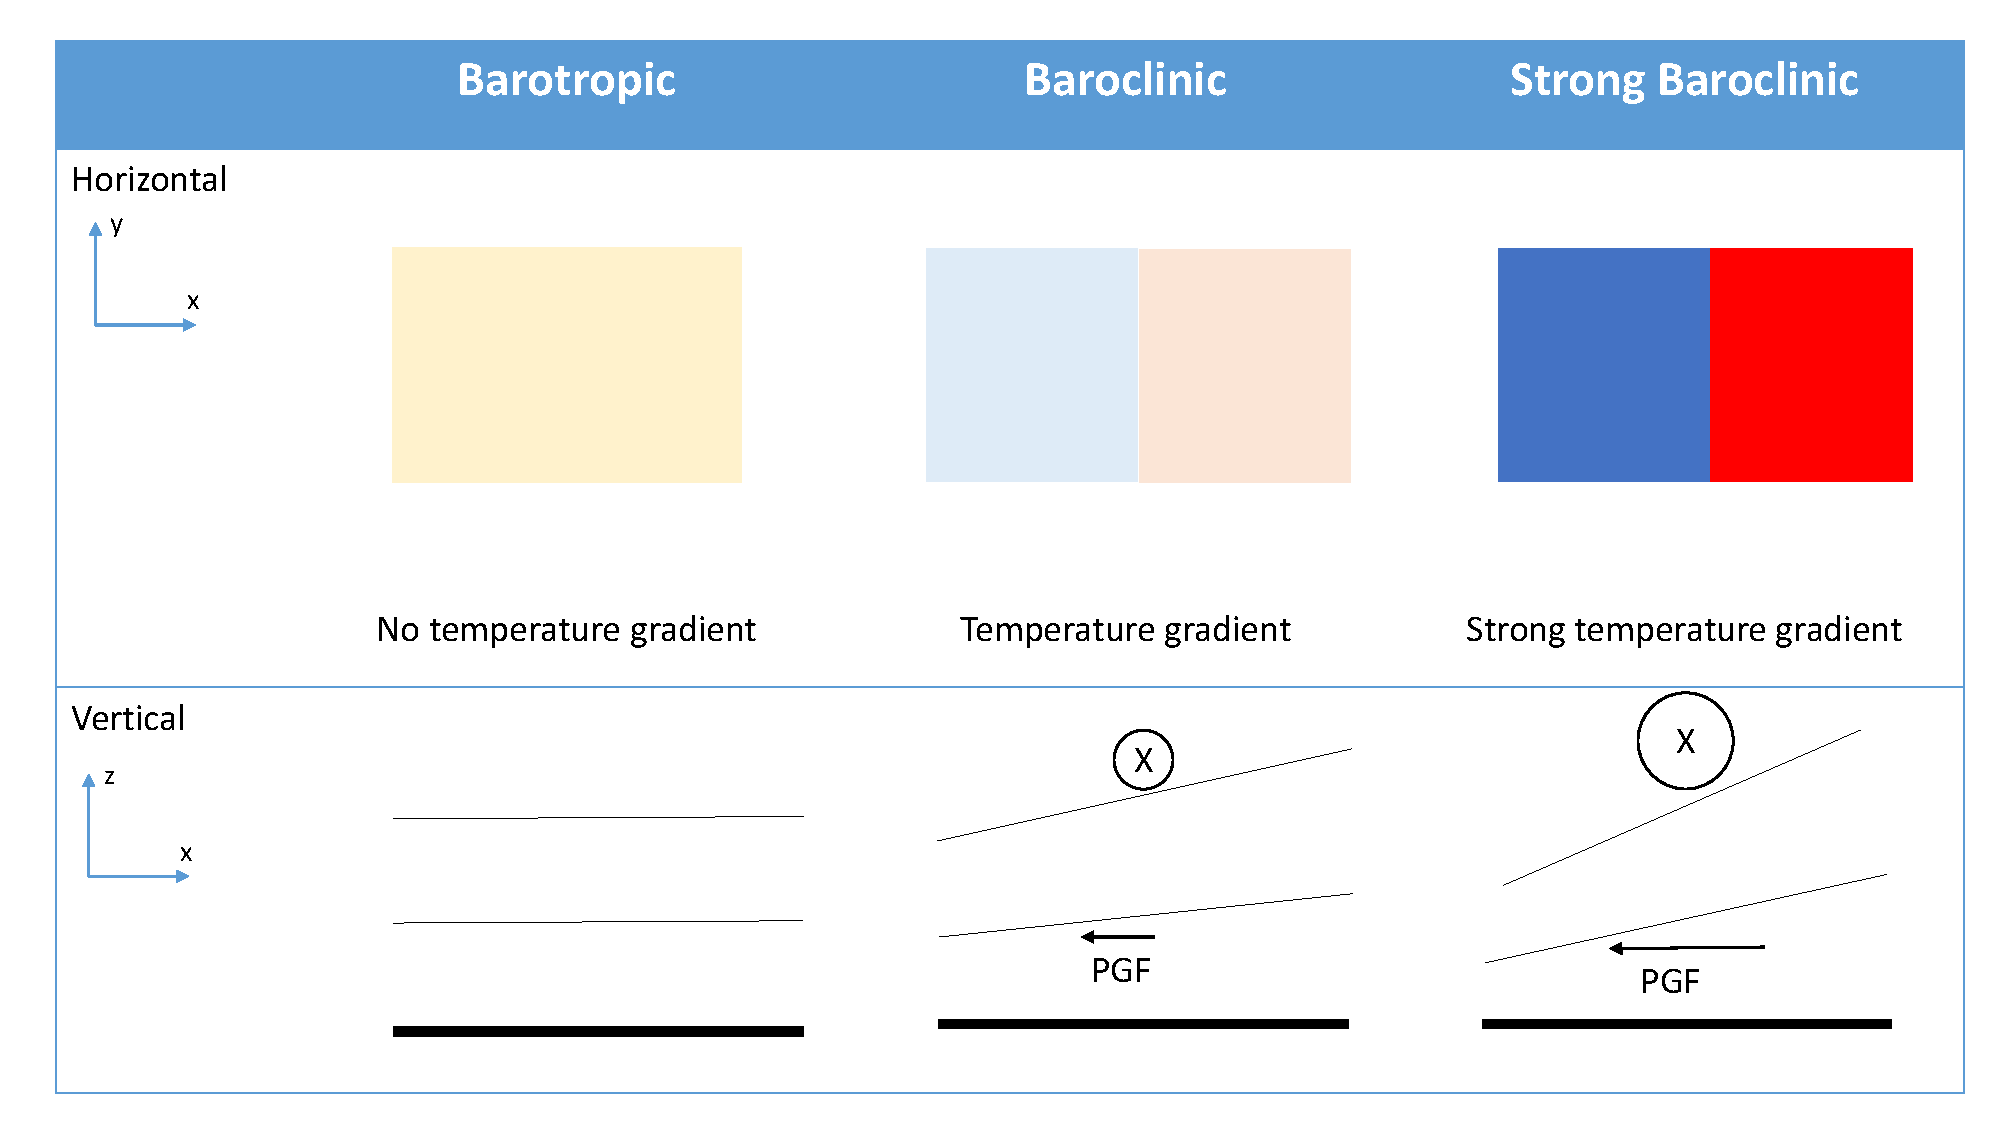
\includegraphics[width=34pc,angle=0]{H:/Documents/Thesis/phd-thesis-template-2.2.2_AC/phd-thesis-template-2.2.2/Figs/barotropic2_new.pdf}
%	\caption{Barotropic and baroclinic environments in the horizontal and vertical, and resultant pressure gradient force (PGF) and thermal wind (cross in circle). Thin black lines are isentropes.}\label{fig:barotropic}
%	\centering
%\end{figure} 

The  M-$\theta$e relationship states that if the $\theta$e surfaces are steeper than the M surfaces, there is symmetric instability. Any slantwise displacement occurring between the slopes of these surfaces will release the symmetric instability and the parcel will be accelerate in the direction away from the original position. Figure \ref{fig:symm_inst} illustrates the M-$\theta$e relationship, with a symmetrically unstable atmosphere on the left and a symmetrically stable atmosphere on the right. Only moist slantwise instability occurs in the Earth's atmosphere \cite{bennetts1979conditional} and so $\theta$e is used. This instability has a 2D assumption that there is no variation in the along front direction. 


\begin{figure}
	\centering	
	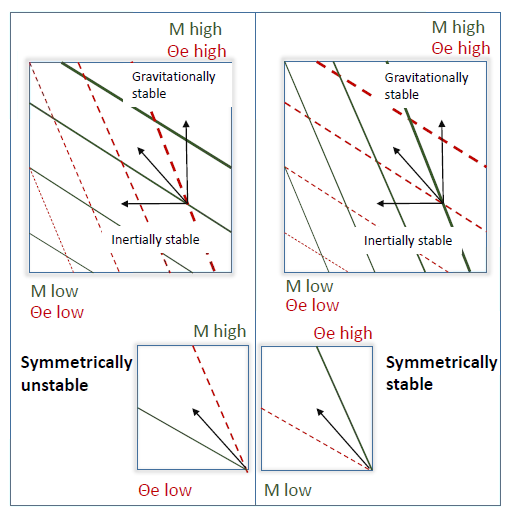
\includegraphics[width=26pc,angle=0]{mocrette_diagram2_screen.png}
	\caption{Shear (symmetric instability). Isentropes are shown in red dashed lines and lines of constant absolute momentum (M) in solid green. Thickness of the lines increases towards  higher values. Both environments are baroclinic and $\theta$e and M are low in the bottom left and high in the top right. The black arrows show direction of movement of air parcels. In both panels a and b, if a parcel is moved to the left, it is inertially stable as it is moving towards an area of reduced absolute momentum. In both panels a and b, if a parcel is moved vertically, they are gravitationally stable as potential temperature is increasing in this direction and so the parcel will return to it's original position. However, in panel a, if an air parcel is moved along arrow x, it is moving towards lower potential temperature and high M, so is symmetrically unstable. In panel b, it will move towards higher $\theta$e and low M, and is symmetrically stable. Modified from \cite{morcrette2004radar}}\label{fig:symm_inst}
\end{figure}


%\begin{figure}
%	\centering	
%	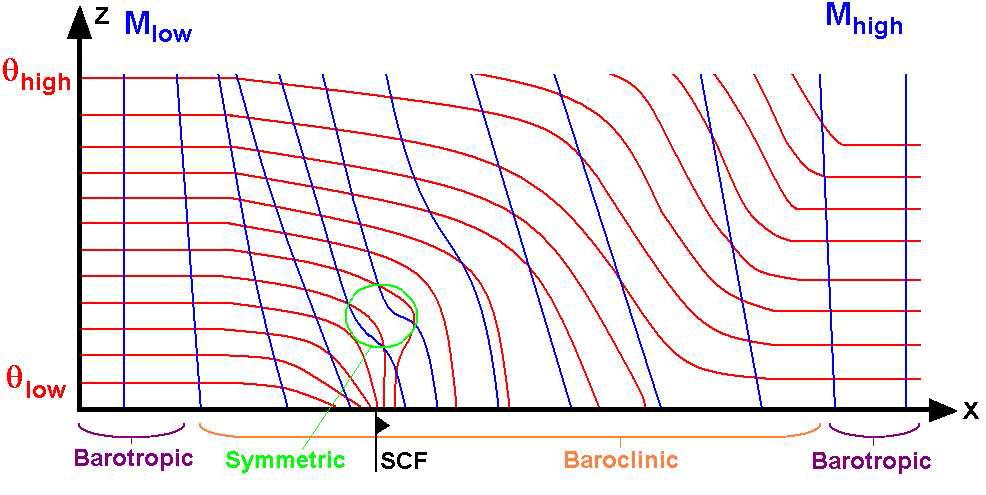
\includegraphics[width=26pc,angle=0]{H:/Documents/Thesis/phd-thesis-template-2.2.2_AC/phd-thesis-template-2.2.2/Figs/morcrette_cx.png}
%	\caption{1.6 The distribution of saturated equivalent potential temperature (red lines) and
%		geostrophic absolute momentum Mg (blue lines) in the broad region around a cold front. Far
%		from the front, the atmosphere is barotropic, within the cold frontal region the atmosphere is
%		increasingly baroclinic, very close to the front, a conditionally symmetrically unstable region
%		may be present. In this example, there is also a small region of conditional instability below
%		the symmetrically unstable region.Source: \cite{morcrette2004radar}}\label{fig:symm_inst2}
%	
%\end{figure}

It has been suggested that slantwise convection from the release of shear instability can explain banded precipitation often seen at cold fronts \citep{bennetts1979conditional, seltzer1985possible}, caused by cells of alternating rotation creating updrafts and downdrafts.

The shear instability diagnostic that is used in this study is diagnosed using:
% dubar/dp x (u'w')bar + dvbar/d[ x (v'w')bar
\begin{equation} \label{eq_diag}
-\overline{w'u'} . \frac{\partial{\overline u}}{\partial z} + \overline{w'v'} . \frac{\partial{\overline v}}{\partial z}
\end{equation}

\begin{equation} \label{eq_diag}
\frac{\partial}{\partial{T}} EKE = -\overline{w'u'} . \frac{\partial{\overline u}}{\partial z} + \overline{w'v'} . \frac{\partial{\overline v}}{\partial z} + ...
\end{equation}

The instability in the x (u) and y (v) directions are combined. The covariance of small-scale vertical motions ($\omega$') and horizontal vertical motions (u' or v') is calculated and then the  product with the vertical shear of low pass winds ($\overline{u}$ or $\overline{v}$)  is created. This is a momentum flux that is purely mechanical and has no dependence on temperature.

%Energy cascade. Also small scale feeds back on the large scale - the diagnostic is the bar value.
%
%Mechanical only.... not like capes????
%Thermodynamic and dynamic mechanism???? what is all this about?
%Shear diagnostic is just vertical and horizontal winds.

%Holton P 279 - symmetric baroclinic instability
%Absolute momentum and potential temperature conservation
%
%WHAT IS MOMENTUM AND ENERGY
%
%\begin{equation} \label{eq_EKE}
%\frac{\overline{(u'^{2}+v'^{2})}}{2} 
%\end{equation}
%EKE in relation to diagnostic?


%Buoyancy (b). g is acceleration due to gravity \(9.8ms^{-1}\). {$\rho$} is density.
%
%\begin{equation} \label{eq_b}
%b = -g\frac{\rho}{\rho_0}
%\end{equation}
%
%Also calculated upright buoyancy (w'{$\alpha$})
%
%Relate to buoyancy and EKE




\subsection{Observations of extra-tropical storms}


\subsection {Representation in models}

%Different results - different identification and tracking, intensity measures \citep{ulbrich2009extra}.

%Climate models (HiGEM (0.83x1.25) and ERA-40) can capture the structural features of extra-tropical cyclones \citep{catto2010can} analysing warm conveyor belt, cold conveyor belt and dry intrusion.

\section {Research question..}
Extra-tropical cyclone activity in the North Atlantic and the relationship with the sea surface temperature in the Gulf Stream region. I will assess whether or not the warm path mechanism (Section 3.3), already examined in one case study \cite{sheldon2017warm}, has relevance to the climatological state of the storm-track in the North Atlantic. I will analyse operational and ensemble forecasts run at ECMWF (1980 to present at a resolution of 9km and 16km, respectively) using diagnostics to isolate the new mechanism that have already been developed. These show the presence of regions of negative PV at mid to upper levels, downgradient vertical momentum fluxes by small spatial scales. The new work proposed here will complement my first years work of statistical analysis with a more physics-based and model-based approach. It will also offer a broader view of how the ocean state affects cyclones worldwide. 

ADD TO ACRONYMS: HRES, AGCM, OGCM.

% from lecturev3 latex doc - looks wrong
%\frac{dQ}{dt} & =0\\
%Q & \equiv\frac{\zeta+f}{H+\eta}


\section {Data}  \label{data}

The data used analysed has been produced by ECMWF. The ERA-Interim reanalysis (ref) and acknowledge and the ECMWF forecast hindcast and forecast, which are described in detail along with the model in section \ref{ECMWF_fs}.

\subsection {ECMWF Integrated Forecasting System (IFS)}  \label{ECMWF_fs}
%www.ecmwf.int/en/forecasts/documentation-and-support is ecmwf_ifs in jabref
%ecmwf_user_guide
%ecmwf_ifs_dynamics
%ecmwf_atm_dyn
%ecmwf_newgrid

The ECMWF Integrated Forecasting System (IFS) consists of an atmospheric general circulation model (AGCM), an ocean general circulation model (OGCM, res), an ocean wave model, a land surface model, along with perturbation models for the data assimilation (EDA) and forecast (ENS) ensembles.

"The dynamical core of IFS is hydrostatic, two-time-level, semi-implicit, semi-Lagrangian and applies spectral transforms between grid-point space (where the physical parametrizations and advection are calculated) and spectral space." \citep{ecmwf_atm_dyn}. In the horizontal, a type of reduced Gaussian grid is used (check the new one is reduced Gaussian), where the separation between longitudinal points is kept almost constant with increasing latitude, by gradually decreasing the number of grid points towards the poles. "For the convenience of computing horizontal derivatives and to facilitate the time-stepping scheme, a spectral representation, based on a series of expansion of spherical harmonics, is used for the prognostic variables" \citep{ecmwf_user_guide}. Vertical resolution is finest in the planetary boundary layer, with sigma levels used that follow the orography of the Earth. These levels transition onto surfaces of constant pressure in the upper levels \citep{ecmwf_user_guide}.

In March 2016, ECMWF  launched a new model cycle, with a new grid comprising up to 904 million prediction points, three times as many as before \citep{ecmwf_newmodel}.
The horizontal grid spacing for high-resolution forecasts has been reduced from 16 km to 9 km, and the ensemble forecasts are now run at 18 km up to forecast day 15 and 36 km thereafter. The vertical grid spacing is unchanged. A new ‘cubic-octahedral grid’ (figure \ref{fig:ecmwf_grid}) pattern is now used and the number of waves used to represent the meteorological fields has been kept the same, while increasing the number of grid points used to represent each wavelength \citep{ecmwf_newmodel}.

\begin{figure}
	
	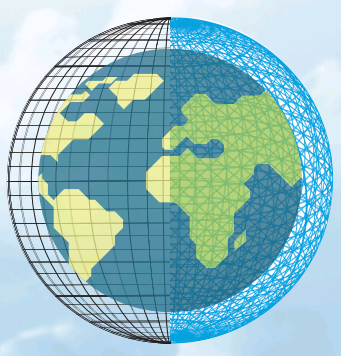
\includegraphics[width=14pc,angle=0]{ecmwf_grid.png}
	\caption{ECMWF grid. Source:\citep{ecmwf_infographic}}\label{fig:ecmwf_grid}
	\centering
\end{figure}


Assimilation of observations using a 4D-Var technique.
Top at 0.1hPa


\begin{landscape}
	
	
	\begin{table}%[h]
		\caption{Some available ECMWF products}\label{t_ecmwf}
		%	\begin{center}
		%	\begin{tabular}{cccccccc} use p to wrap text
		\begin{tabular}{ | p{3.5cm} | p{2.5cm}|  p{1.5cm} | p{2.5cm}|  p{2.5cm} |  p{2.5cm}| p{2.5cm} | }
			\hline\hline
			Forecast & Type & Days & Atmospheric horizontal resolution & Atmospheric vertical resolution & SST & Run times \\
			\hline\hline
			High resolution (deterministic) & Operational & 0-10 & \textasciitilde{9} km & 137 levels & OSTIA Persisted SSTs & 0Z, 12Z \\ %% $ $ is math mode - put this around the bits that are not text
			\hline
			
			Ensemble         (51 members) & Operational  & 0-15 & \textasciitilde{18} km &  91 levels & NEMO 0.25$^0$  & 0Z, 12Z \\
			Ensemble         (51 members) & Operational & 16-46 & \textasciitilde{32} km &  91 levels & NEMO 0.25$^0$  & Mon, Thurs \\
			
			\hline
			Ensemble         (11 members) & Hindcast & 0-15 & 0.2$^0$ \textasciitilde{18} km &  91 levels & ERA-Interim & Mon, Thurs  \\
			Ensemble         (11 members) & Hindcast & 16-46 & \textasciitilde{32} km &  91 levels & ERA-Interim & Mon, Thurs  
			\\			
			\hline\hline
			ERA-Interim & Reanalysis & 1979 - present & 0.75$^0$ \textasciitilde{79} km & 60 levels & various & ongoing \\
			
			\hline
		\end{tabular}
		%\end{center}
	\end{table}
\end{landscape}


\subsubsection {Ensemble forecast hindcast}  \label{ECMWF_hindcast}
A hindcast, or reforecast is a model forecast run initialised with conditions in the past. The current version of the ECMWF model is given .. data based on xx of a day in the past and then runs forwards as a forecast. This provides a way to calibrate the output.
Skill evaluation and calibration - the model drifts, so need to estimate from the model climate. Do not issue forecasts directly from the model, use anomalies.
Reforecasts initialised from ERA-Interim, not OSTIA.

Hindcast starts every Monday and Thursday, for that day over the past 20 years (to 1996). These hindcast ensembles consist of 1 control run and 10 perturbed ensemble members and run for 46 days, with resolution decreasing at day 16 ? or 11?

"To account for initial uncertainties, the oceanic Control temperature analysis, including the SST and the deep ocean temperature, is complemented by four alternative analyses. They are produced by adding randomly chosen wind perturbations to the ocean data assimilation, driven by five slightly different meteorological fields based on the Control analysis, slightly and randomly perturbed. The resulting five ocean analyses are then distributed among the Control and ensemble members."

\begin{figure}
	
	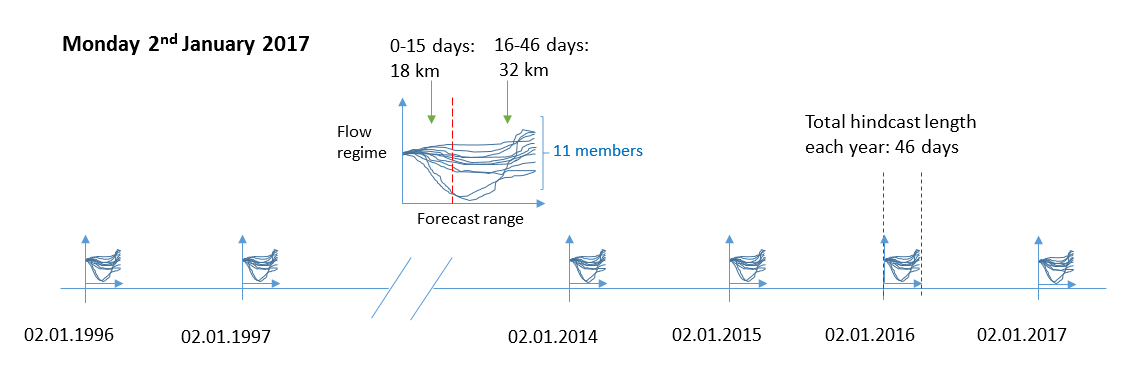
\includegraphics[width=34pc,angle=0]{ec_hindcast2.png}
	\caption{An example of the ECMWF hindcast schedule. For example, on Monday 2nd January 2017, 20 hindcast years (back to 1996) will be run. Each ensemble is made up of 11 members that reduce in resolution at day 15. (or day 10?) and run for a total of 46 days.}\label{fig:ecmwf_hindcast}
	\centering
\end{figure}

Over a year, with a model run on every Monday and Thursday for ... days, an entire 20 year period with xxx ensembles will have been created.

Hindcasts are a useful product to use......

A hindcast, or reforecast is a model forecast run initialised with conditions in the past. The hindcast run commences every Monday and Thursday, for that day for the past 20 years (to 1996) (figure \ref{fig:hindcast}).


Over a year, with a model run on every Monday and Thursday, an entire 20 year period with 10 ensembles members plus the control will have been created. Resolution of all of the members decreases at day 16. The initial 15 days of the hindcast that are analysed here have a resolution of 0.2$^0$. The ensemble members have five different ocean temperature analyses, with members 1 and 6, 2 and 7, 3 and 8, 4 and 9, 5 and 10 sharing the same initial state. These perturbed states are produced by adding randomly chosen wind perturbations to the ocean data assimilation, driven by five slightly different meteorological fields based on the control analysis.

For the ocean, we use 5 different ocean re-analyses (control + 4 perturbed) which are used to perturb the 11 members - which means that there are pairs of members which share the same SSTs as you said.

atmosphere: Singular vectors are applied in the Extratropics + Ensemble data assimilation (EDA) perturbations everywhere.

No, the atmospheric model is also perturbed using stochastic perturbations (SPPT scheme and also back-scatter scheme for the model version you are using), but only for the perturbed forecasts. The control forecast (type  cf or ensemble 0) is not perturbed. 

(Frederic email 9 Nov)
%What about the different atmosphere or model parts?
%The current version of the ECMWF model is given .. data based on xx of a day in the past and then runs forwards as a forecast. This provides a way to calibrate the output.
%Skill evaluation and calibration - the model drifts, so need to estimate from the model climate. Do not issue forecasts directly from the model, use anomalies.
%Reforecasts initialised from ERA-Interim, not OSTIA.

%% Analysis and model physics perturbed  https://www.ecmwf.int/en/forecasts/documentation-and-support#reforecasts
%ensemble members lower res???  na... all 18 km ??
%


\subsubsection {Operational forecast}  \label{ECMWF_forecast}
The high resolution (deterministic) operational forecast uses an atmosphere-only GCM. SSTs come from the Operational Sea Surface Temperature and Sea Ice Analysis (OSTIA) analysis at day 0, which persist throughout the forecast window (days 0-10). This is a high resolution analysis of the SST for the global ocean with daily, global coverage 1/20$^0$ ($\tilde{6}$ km) combined SST and sea ice concentration product, which is generated in near real time \citep{donlon2012operational}.

\begin{table}%[h]
	\caption{Operational forecast resolution}\label{t_ecmwf2}
	%	\begin{center}
	%	\begin{tabular}{cccccccc} use p to wrap text
	\begin{tabular}{ ccc }
		\hline\hline
		Date & Grid & Horizontal resolution \\
		\hline\hline
		21.11.00 & N256 & 0.5$^0$ \textasciitilde{40} km \\ %% $ $ is math mode - put this around the bits that are not text
		01.02.06 & N400 & 0.225$^0$ \textasciitilde{25} km \\ %% $ $ is math mode - put this around the bits that are not text
		26.01.10 & N640 & 0.125$^0$ \textasciitilde{16} km \\ %% $ $ is math mode - put this around the bits that are not text
		08.03.16 & O1280 & 0.1$^0$ \textasciitilde{9} km \\ %% $ $ is math mode - put this around the bits that are not text		
		\hline
	\end{tabular}
	%\end{center}
\end{table}

The grid used for the operational forecasts is updated every \textasciitilde{6} years and is currently being run at 0.1$^0$ resolution (table \ref{t_ecmwf2}).
%What is the spectral resolution??
%
%The sst and sea ice are updated during the model integration according to the tendency obtained from climatology of OSTIA (5km) \citep{ecmwf_user_guide}.
%
%The ensemble forecast (days 0-10) is at half the horizontal resolution and also has fewer levels in the vertical.  During these initial 10 days, the forecast uses an atmosphere-only GCM, with OSTIA SSTs. Five different ocean analyses are distributed amongst the control and ensemble members, produced by adding wind perturbations from different meteorological fields. \citep{ecmwf_user_guide}.  From days 10-46, the horizontal resolution of the ensemble is reduced to half (to 32 km) and the atmosphere is coupled to the NEMO ocean model \citep{madec2015nemo}. 
%The 50 ensemble members are formed by making small changes to the 4D-VAR analysis, creating perturbed initial states \citep{ecmwf_user_guide}.
%
%How are the ensembles generated - different ocean initial state and atmospheric initial state??
%
%ensemble forecast:
%The horizontal resolution of the ensemble is reduced at day 10, and the remainder of the forecast (out to 15 or 32 days) is run at half the resolution of the first 10 days.
%No ocean coupling for the first 10 days. From day 10 onwards, coupled to ocean model (5 ocean analyses for initial conditions).
%
%
%"The ocean-atmosphere coupling is achieved by a two-way interaction: the atmosphere affects the ocean through its wind, heat and net precipitation (precip-evap), whilst the ocean affects the atmosphere through its SST. for the ENS, this interaction is every hour" \citep{ecmwf_user_guide}.
%
%With respect to synoptic patterns, the control ensemble forecast  gives a similar performance to HRES, which is at twice the resolution \citep{ecmwf_user_guide}. However, HRES is better at forecasting small-scale extreme events, for example strong winds and heavy rain, when resolution is more important. 
%
%The high resolution model will be coupled to NEMO 0.25$^0$ at the end of 2017.
%Verification against ERA-Interim.
%Archived at the resolution run at.


The high resolution (deterministic) operational forecast uses an atmosphere-only GCM. SSTS come from the Operational Sea Surface Temperature and Sea Ice Analysis (OSTIA) analysis at day 0, which persist throughout the forecast window (days 0-10). This is a high resolution analysis of the SST for the global ocean with daily, global coverage 1/20° (~6 km) combined SST and sea ice concentration product, which is generated in near real time \citep{donlon2012operational}.
What is the spectral resolution??

The sst and sea ice are updated during the model integration according to the tendency obtained from climatology of OSTIA (5km) \citep{ecmwf_user_guide}.

The ensemble forecast (days 0-10) is at half the horizontal resolution ( x compared to x) and also has fewer levels in the vertical.  During these initial 10 days, the forecast uses an atmosphere-only GCM, with OSTIA SSTs. Five different ocean analyses are distributed amongst the control and ensemble members, produced by adding wind perturbations from different meteorological fields. \citep{ecmwf_user_guide}.  From days 10-46, the horizontal resolution of the ensemble is reduced to half (to 32 km) and the atmosphere is coupled to the NEMO ocean model \citep{madec2015nemo}. 
The 50 ensemble members are formed by making small changes to the 4D-VAR analysis, creating perturbed initial states \citep{ecmwf_user_guide}.

How are the ensembles generated - different ocean initial state and atmospheric initial state??

ensemble forecast:
The horizontal resolution of the ensemble is reduced at day 10, and the remainder of the forecast (out to 15 or 32 days) is run at half the resolution of the first 10 days.
No ocean coupling for the first 10 days. From day 10 onwards, coupled to ocean model (5 ocean analyses for initial conditions).


"The ocean-atmosphere coupling is achieved by a two-way interaction: the atmosphere affects the ocean through its wind, heat and net precipitation (precip-evap), whilst the ocean affects the atmosphere through its SST. for the ENS, this interaction is every hour" \citep{ecmwf_user_guide}.

With respect to synoptic patterns, the control ensemble forecast  gives a similar performance to HRES, which is at twice the resolution \citep{ecmwf_user_guide}. However, HRES is better at forecasting small-scale extreme events, for example strong winds and heavy rain, when resolution is more important. 

The high resolution model will be coupled to NEMO 0.25$^0$ at the end of 2017.
Verification against ERA-Interim.
Archived at the resolution run at.


\begin{table}%[h]
	\caption{Operational forecast resolution}\label{t_ecmwf2}
	%	\begin{center}
	%	\begin{tabular}{cccccccc} use p to wrap text
	\begin{tabular}{ ccc }
		\hline\hline
		Date & Grid & Horizontal resolution \\
		\hline\hline
		21.11.00 & N256 & 0.5$^0$ \textasciitilde{40} km \\ %% $ $ is math mode - put this around the bits that are not text
		01.02.06 & N400 & 0.225$^0$ \textasciitilde{25} km \\ %% $ $ is math mode - put this around the bits that are not text
		26.01.10 & N640 & 0.125$^0$ \textasciitilde{16} km \\ %% $ $ is math mode - put this around the bits that are not text
		08.03.16 & O1280 & 0.1$^0$ \textasciitilde{9} km \\ %% $ $ is math mode - put this around the bits that are not text		
		\hline
	\end{tabular}
	%\end{center}
\end{table}

The grid used for the operational forecasts is updated every \textasciitilde{6} years and is currently being run at 0.1$^0$ resolution (table \ref{t_ecmwf2}).
%What is the spectral resolution??
%
%The sst and sea ice are updated during the model integration according to the tendency obtained from climatology of OSTIA (5km) \citep{ecmwf_user_guide}.
%
%The ensemble forecast (days 0-10) is at half the horizontal resolution and also has fewer levels in the vertical.  During these initial 10 days, the forecast uses an atmosphere-only GCM, with OSTIA SSTs. Five different ocean analyses are distributed amongst the control and ensemble members, produced by adding wind perturbations from different meteorological fields. \citep{ecmwf_user_guide}.  From days 10-46, the horizontal resolution of the ensemble is reduced to half (to 32 km) and the atmosphere is coupled to the NEMO ocean model \citep{madec2015nemo}. 
%The 50 ensemble members are formed by making small changes to the 4D-VAR analysis, creating perturbed initial states \citep{ecmwf_user_guide}.
%
%How are the ensembles generated - different ocean initial state and atmospheric initial state??
%
%ensemble forecast:
%The horizontal resolution of the ensemble is reduced at day 10, and the remainder of the forecast (out to 15 or 32 days) is run at half the resolution of the first 10 days.
%No ocean coupling for the first 10 days. From day 10 onwards, coupled to ocean model (5 ocean analyses for initial conditions).
%
%
%"The ocean-atmosphere coupling is achieved by a two-way interaction: the atmosphere affects the ocean through its wind, heat and net precipitation (precip-evap), whilst the ocean affects the atmosphere through its SST. for the ENS, this interaction is every hour" \citep{ecmwf_user_guide}.
%
%With respect to synoptic patterns, the control ensemble forecast  gives a similar performance to HRES, which is at twice the resolution \citep{ecmwf_user_guide}. However, HRES is better at forecasting small-scale extreme events, for example strong winds and heavy rain, when resolution is more important. 
%
%The high resolution model will be coupled to NEMO 0.25$^0$ at the end of 2017.
%Verification against ERA-Interim.
%Archived at the resolution run at.

\subsubsection {ERA-Interim reanalysis}  \label{ECMWF_ERA}


\begin{table}[h]
	\caption{Variables}\label{t_variables}
	\begin{center}
		\begin{tabular}{ccc}
			
			\hline\hline
			$Variable$ & $Units$ & $Pressure Levels (hPa)$ \\
			\hline
			Zonal wind (u) & ms$^-1$ & 300, 400, 500, 700, 850, 925, 1000 \\ %% $ $ is math mode - put this around the bits that are not text
			Meridional wind (v) & ms$^-1$ & 300, 400, 500, 700, 850, 925, 1000  \\
			Vertical .. (w) & ms$^-1$ & 300, 400, 500, 700, 850, 925, 1000  \\
			Temperature (t) & K & 300, 400, 500, 700, 850, 925, 1000 \\
			Potential temperature (theta) & ms & 300, 400, 500, 700, 850, 925, 1000  \\
			q (q) & ms & 300, 400, 500, 700, 850, 925, 1000  \\
			Potential vorticity (PV) & ms & N/A  \\
			Geopotential height (Z) & ms & xx  \\
			
			\hline
		\end{tabular}
	\end{center}
\end{table}
% available at 50, 100, 200, 300, 400, 500, 700, 850, 925, 1000
Specific Humidity, Quasi-geostrophic Potential Vorticity, Water Vapor Mixing Ratio

At 6-hourly temporal resolution, time step 0 to 360, which is 10 days.

ERA-Interim is a global atmospheric reanalysis from 1979, continuously updated in real time. The spatial resolution of the data set is approximately 80 km (T255 spectral) on 60 vertical levels from the surface up to 0.1 hPa \citep{dee2011era}.

%http://www.ecmwf.int/en/research/modelling-and-prediction/atmospheric-dynamics
%"The wave model at ECMWF is called the “WAM”. It describes the rate of change of the 2- dimensional wave spectrum, in any water depth, caused by advection, wind input, dissipation due to white capping and bottom friction and non-linear wave interactions. It is set up so as to allow the two-way interaction of wind and waves with the atmospheric model. It is also incorporated in the medium-range, monthly and seasonal ensembles. 
%Radar altimeter wave-height data are assimilated from satellites. Buoy wave data are not assimilated; instead, they serve as an independent check on the quality of modelled wave parameters. The propagation of swell in the wave model is handled by a simple scheme that gives rise to a smoothing of the wave field. At present the effects of surface currents on the sea state are not taken into account. In particular areas, such as the Gulf Stream or Agulhas current, the current effect may give rise to localised changes of up to one metre in the wave height. The representation of the sea-ice fields is not as accurate as would be needed to handle waves near the ice edge. Due to the present model resolution, wave products near the coasts and, to a lesser extent, in small enclosed basins (e.g. the Baltic Sea) may be of lower quality than the open-ocean products. "
%Tides?

"The OGCM can reproduce the general features of the circulation and the thermal structure of the upper layers of the ocean and its seasonal, but has systematic errors, some of which are caused by the coarse vertical and horizontal resolution: the model thermocline is too diffuse; the Gulf Stream does not separate at the right location. (ref online guide).
The ocean analysis is performed every 10 days, down to a depth of 2000 m. The ocean-atmosphere coupling is achieved by a two-way interaction: the atmosphere affects the ocean through its wind, heat and net precipitation (precipitation-evaporation), whilst the ocean affects the atmosphere through its SST. For ENS, this interaction is every hour. what about regular forecast? not needed?? "


\begin{figure}
	
	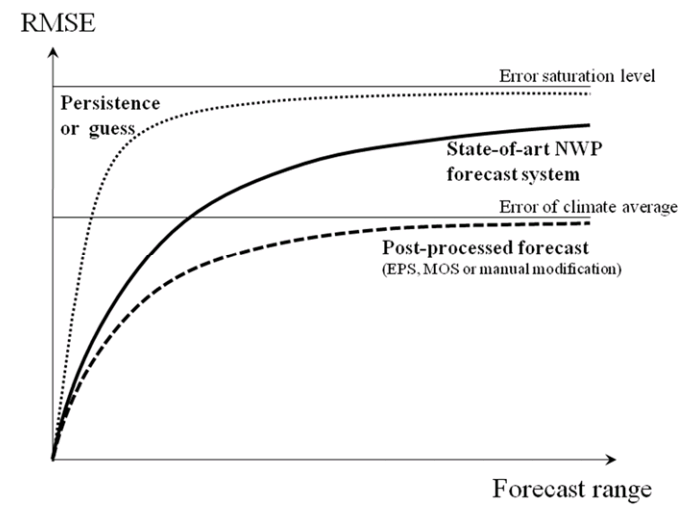
\includegraphics[width=22pc,angle=0]{forecast_error.png}
	\caption{Forecast error. From ECMWF web guide}\label{fig:forecast_error}
	\centering
\end{figure}


More details about spectral and truncation. Spectral and grids...
Parametrisation scheme...
global
hydrostatic - pressure coordinates?

%I will be looking at the medium-range(3-10 days). ECMWF’s forecasts cover time frames ranging from medium-range (3-10 days), to monthly and seasonal, and up to a year ahead.
%Nowcasting (0 - 6 hours)
%Short-range weather forecasts (1 - 3 days)
%Medium-range weather forecasts (3 - 10 days)

%"Between day 9 and day 10 there is a 24-hour overlap period, to reduce the “shock” of the change, in particular for the parameters that are most sensitive, for example convection and large-scale precipitation. Accumulations of precipitation (and other fluxes) for periods that span the resolution change (day 10) need to use low-resolution data from the overlap period and such data is thereforeavailable via dissemination."

%Not dealt with 'Forecasts from 15 to 32 days'

ERA-5 reanalysis download at 0.25 degree resolution
https://software.ecmwf.int/wiki/display/CKB/ERA5+data+documentation

% https://software.ecmwf.int/wiki/display/CKB/Does+downloading+data+at+higher+resolution+improve+the+output

For ERA-Interim the point interval on the native Gaussian grid is about 0.75 degrees (with the exception of Ocean-Wave data which are natively stored on the wave model’s reduced 1.0x1.0 degrees latitude/longitude grid). You can specify a custom grid on the data server web interface, or using the ECMWF WebAPI or using the MARS client (if you have access to it).  On the web interface the default grid for ERA-Interim is lat/long, with a default resolution of 0.75x0.75 degrees (about 80km), approximating the irregular grid spacing on the native Gaussian grid.

For ERA5 data the point interval on the native Gaussian grid is about 0.28 degrees. You can download ERA5 data using Python and specify a custom grid and resolution in your script. You should set the horizontal resolution to slightly lower than 0.28 degrees (about 30km), for example to 0.25 degrees, approximating the irregular grid spacing on the native Gaussian grid.



\subsection{Ensemble forecasting}

A hindcast, or reforecast is a model forecast run initialised with conditions in the past. The hindcast run commences every Monday and Thursday, for that day for the past 20 years (to 1996) (figure \ref{fig:hindcast}).

\begin{figure} [h]
	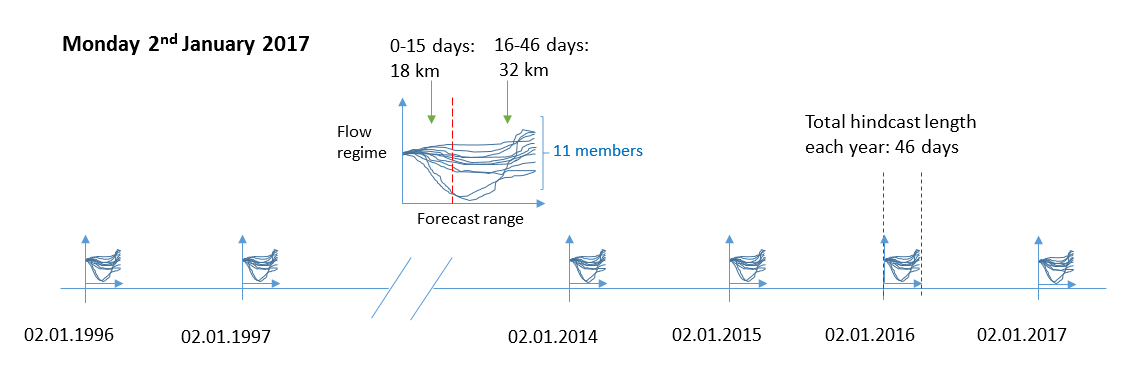
\includegraphics[width=34pc,angle=0]{ec_hindcast2.png}
	\caption{An example of the ECMWF hindcast schedule. For example, on Monday 2nd January 2017, 20 hindcast years (back to 1996) will be run. Each ensemble is made up of 11 members that reduce in resolution at day 15 and run for a total of 46 days.}\label{fig:ecmwf_hindcast}
	\centering
\end{figure} \label{fig:hindcast}	

Over a year, with a model run on every Monday and Thursday, an entire 20 year period with 10 ensembles members plus the control will have been created. Resolution of all of the members decreases at day 16. The initial 15 days of the hindcast that are analysed here have a resolution of 0.2$^0$. The ensemble members have five different ocean temperature analyses, with members 1 and 6, 2 and 7, 3 and 8, 4 and 9, 5 and 10 sharing the same initial state. These perturbed states are produced by adding randomly chosen wind perturbations to the ocean data assimilation, driven by five slightly different meteorological fields based on the control analysis.

For the ocean, we use 5 different ocean re-analyses (control + 4 perturbed) which are used to perturb the 11 members - which means that there are pairs of members which share the same SSTs as you said.

atmosphere: Singular vectors are applied in the Extratropics + Ensemble data assimilation (EDA) perturbations everywhere.

No, the atmospheric model is also perturbed using stochastic perturbations (SPPT scheme and also back-scatter scheme for the model version you are using), but only for the perturbed forecasts. The control forecast (type  cf or ensemble 0) is not perturbed. 

(Frederic email 9 Nov)
%What about the different atmosphere or model parts?
%The current version of the ECMWF model is given .. data based on xx of a day in the past and then runs forwards as a forecast. This provides a way to calibrate the output.
%Skill evaluation and calibration - the model drifts, so need to estimate from the model climate. Do not issue forecasts directly from the model, use anomalies.
%Reforecasts initialised from ERA-Interim, not OSTIA.

%% Analysis and model physics perturbed  https://www.ecmwf.int/en/forecasts/documentation-and-support#reforecasts
%ensemble members lower res???  na... all 18 km ??
%
%Hindcasts are a useful product to use......


Poor forecasts result from errors in initial conditions and model errors, with initial conditions dominating during the first five days or so. "Analysis errors amplify most easily in the sensitive parts of the
atmosphere, in particular where strong baroclinic systems develop. These errors then move
downstream and amplify and thereby affect the large-scale flow. To estimate the effect of
possible initial analysis errors and the consequent uncertainty of the forecasts, small changes
to the 4D-Var analysis are made, creating an ensemble of many (currently 50) different,
“perturbed”, initial states. Model deficiencies are represented by a stochastic process. In order
to save computational time, the ensemble members are run with a lower resolution version of
the IFS. 
If the ensembles agree, it is a predictable state. If diverge significantly from each other and the control, less certain forecast. Also calculate the ensemble mean (EM). ENS provides information from which the probability of alternative
developments is calculated, in particular those related to risk of extreme or high-impact
weather. The three methods for creating the ensemble...

%\begin{figure}
%	
%	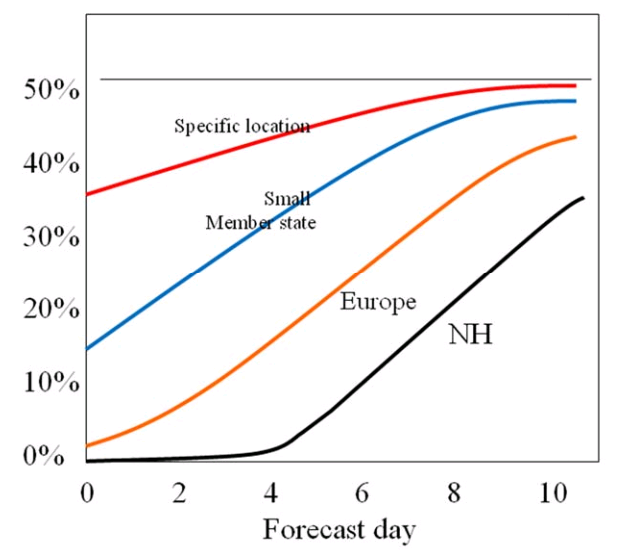
\includegraphics[width=22pc,angle=0]{H:/Documents/Thesis/phd-thesis-template-2.2.2_AC/phd-thesis-template-2.2.2/Figs/ens_pert.png}
%	\caption{Ensemble perturbation}\label{fig:ens_pert}
%	\centering
%\end{figure}

\begin{figure}
	
	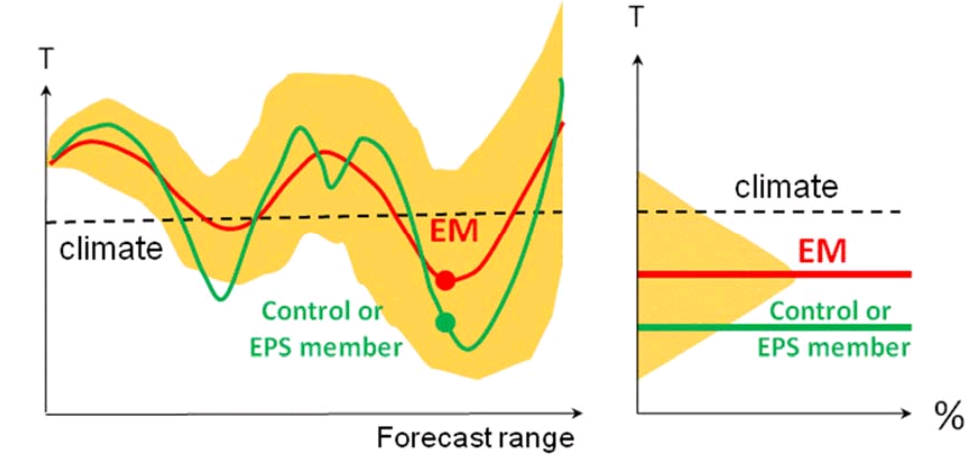
\includegraphics[width=22pc,angle=0]{ens_spread.png}
	\caption{Ensemble spread}\label{fig:ens_spread}
	\centering
\end{figure}

minobe2010atmospheric
kelly2010western
kwon2010role
Molteni, Corti, Palmer, Mike Wallace

%\subsection{The North Atlantic Oscillation}


\subsubsection {ERA5 reanalysis}  \label{ECMWF_ERA5}
% https://software.ecmwf.int/wiki/display/CKB/What+is+ERA5
ERA5 is the 5th major global reanalysis produced by ECMWF.
ERA5 uses the same 37 pressure levels as ERA-Interim.
All parameters available in ERA-Interim are also available in ERA5; and ERA5 has some additional parameters.
10 ensemble members, and also ensemble mean and spread for all parameters and levels are being produced. The temporal resolution is 3-hourly, rather than hourly for the deterministic ERA5 product, though.

%%%%%%%%%%%%%%%%%%%%%%%%%%%%%%%%%%%%%%%%%%%%%%%%%%%%%%%%%%%%%%%%%%%%%%

%*******************************************************************************
%****************************** Second Chapter *********************************
%*******************************************************************************
\chapter{Study}  

\section{Aims}
\begin{itemize}
	\item To explore the seasonal predictability of tropical storms in southern and central China
	\item Examine SST correlations up 17 months prior to the storm season
	\item Propose physical mechanisms by which SST offers seasonal predictability at long lead times

\end{itemize}

\section{Methods}
\subsection{Tropical storm data}

The Joint Typhoon Warning Center (JTWC) Best Track dataset provides the tropical storm data and was obtained from the IBTrACS database (Knapp et al, 2010). Any storms in the West Pacific that have a start time during the months of June to October and have a maximum intensity of least 34 knots (17 m/s, 38 mph) are selected. The dataset includes data on the position, maximum sustained winds, and minimum central pressure for every tropical cyclone globally at 6-hr intervals in UTC.

%The wind speed reported in this dataset is the maximum sustained wind over the 6 hourly time step?? also gusts?@!!! CHECK MSW used

\begin{figure}[h]
	\centering
	\noindent\includegraphics[width=20pc,angle=0]{Y:/Code_Data/Chapter1/Plots/Maps/China_domain.png}
	\caption{Domain marking landfalling storms in the southern and central China domain}\label{fig:landfall_domain}
\end{figure}

All of the storms that intersect a domain encompassing parts of southern and central China (figure \ref{fig:landfall_domain}) from 1958-2014 were chosen for further analysis. Although this includes data from the pre-satellite era, only landfalling storms are examined, and it is likely that these were recorded in the early periods.
%1958 is in the pre-satellite era, only landfalling storms are analysed and these were most likely recorded. The longer the time series the better.

The storms were separated into three categories based on maximum wind speed whilst within the specified domain based on the Saffir-Simpson Hurricane Scale (SSHS). Low intensity storms include tropical depressions and tropical storms (up to 63 knots, 32 m/s, 73 mph). Medium intensity include category one, and two storms from the SSHS (up to 95 knots, 49 m/s, 110 mph). High intensity storms were any that had a higher wind speed.

The standard temporal resolution of storm data is 6-hourly, however, at times there are missing time steps or additional data at a higher frequency. Storm data was interpolated onto a 6-hourly time period, for the calculation of accumulated cyclone energy (ACE), which is used as a proxy for damage. ACE is a value proportional to the energy of the system and is used to express the activity of individual TCs as well as entire TC seasons. The ACE of a season is the sum of the ACEs for each storm and takes into account the number, strength, and duration of all the tropical storms in the season. ACE is calculated by summing the squares of the maximum wind speed (knots) every 6 hours when the TC is within the domain of influence and is in 10\textsuperscript{4} knots\textsuperscript{2}. 

% outside maths mode use textsuperscript instead 10^{4}  	

\begin{equation}
ACE = 10^{-4}	 \sum v^2max
\end{equation}

Total ACE for the entire JJASO season for each year within the specified domain was calculated and will be referred to as ACE-JJASO. This a time series of one value for each season for 57 years (1958-2014).

Power Dissipation Index (PDI) is an alternative measure of tropical cyclone destructiveness, and uses the cube of the maximum wind speed rather than the square. PDI units are 10\textsuperscript{4} knots\textsuperscript{3}. PDI is like ACE but puts more emphasis on storm intensity.
%What is the advantage?
% This has shown to have some skill... cost of cyclones goes up with cube of the wind speed. (Southern reference in Emanuel 2005 Nature paper).
\begin{equation}
PDI = 10^{-4}	 \sum v^3max
\end{equation} 	 


\subsection{Large-scale environmental data}

The large-scale environment data comes from various reanalysis datasets (\ref{t1}). The NCEPNCAR reanalysis \citep{kalnay1996ncep} and JRA-55 reanalysis \citep{kobayashi2015jra} provide the atmospheric data. The NCEPNCAR data extends back until 1948 and has been used in numerous previous studies examining the statistical relationship between the large-scale environment and tropical storm activity. JRA-55 is a more recent reanalysis produced by the Japanese Meteorological Agency (JMA) and is also at higher resolution than the NCEPNCAR dataset.

The SST data from Extended Reconstructed SST (ERSSTv4) dataset \citep{huang2015extended} covers over 150 years, starting in 1854. With the increased availability of sub-surface ocean observations, there are recent reanalyses that included data on ocean heat content. The NCEPCFSR coupled reanalysis \citep{saha2010ncep} provides the tropical cyclone heat potential (TCHP) data, which is the ocean heat content down to the 26$^0$C isotherm, however, data is only available from 1979 - 2010. This TCHP data also only extends to areas with tropical cyclone activity. An alternative product for data on the deeper ocean is the ORSA4 reanalysis \citep{balmaseda2013evaluation}, produced by ECMWF. Ocean heat content (OHC) data to a variety of depths is available, the shallowest being 100m, which was used.

% http://tex.stackexchange.com/questions/47324/superscript-outside-math-mode

\begin{table}[h]
	\caption{Details of data used}\label{t1}
	\begin{center}
		\begin{tabular}{cccc}
			\hline\hline
			$Dataset$ & $Variable$ & $Resolution (grid points)$ & $Years$ \\
			\hline
			JRA-55 & *atmosphere & T319 L60 1.25$^0$ & 1958-2013 \\ %% $ $ is math mode - put this around the bits that are not text
			\citep{kobayashi2015jra} & & (145 x 288) & \\
			NCEPNCAR & *atmosphere & T62 L28 2.5$^0$ & 1948-2014 \\
			\citep{kalnay1996ncep} & & & \\
			ERSSTv4 & SST & 2$^0$ & 1970-2014 \\
			\citep{huang2015extended} & & (89 x 180) & \\
			NCEPCFSR & TCHP & T382 L64 0.5x0.5$^0$ & 1979-2009  \\
			\citep{saha2010ncep} & & & \\
			ORSA4 & OHC & Refined at Tropics 0.3x0.3$^0$ & 1958-2009  \\
			\citep{balmaseda2013evaluation} & & (180 x 360) & \\
			
			\hline
		\end{tabular}
	\end{center}
\end{table}

% nCEP-CFSR(38km)
* atmosphere included mean sea level pressure, relative vorticity, relative humidity, u wind, v wind, precipitable water.

Monthly means of the variables were created, along with monthly tendencies and means of multiple months, e.g. JFM, MAM.


\subsection{Correlation analysis}

To produce correlation maps, the ACE or frequency time series was correlated with the time series of the variable at each grid point. The Pearson R value is a measure of the linear dependence between two variables, giving a value between plus 1 and minus 1 inclusive, where 1 is total positive linear correlation and minus 1 is total negative linear correlation.

The Pearson product moment correlation coefficient is calculated as follows:
%https://data.vanderbilt.edu/biosproj/CI2/corr.tex

$r = \frac{\Sigma(x_i - \bar{x})(y_i - \bar{y})}{\sqrt{\Sigma(x_i - \bar{x})^2\Sigma(y_i - \bar{y})^2}}$

The Pearson R value gives information on the direction and strength of correlation (\ref{tcorrs}). % with 0.3-0.4 OR 0.5 weak then moderate then strong >0 being very strong, in between is moderate.

\begin{table} % remove [h] and sits in right place
	\caption{Interpretation of Pearson R correlation coefficient}\label{tcorrs}
	\begin{center}
		\begin{tabular}{cc}
			\hline\hline
			Correlation coefficient R & Correlation strength \\
			\hline
			.70 or higher & very strong  \\ 
			.40 to +.69 & strong \\ 
			.30 to +.39 & moderate  \\
			.20 to +.29 & weak \\
			
			\hline
		\end{tabular}
	\end{center}
\end{table}


This coefficient is accompanied by a p-value, which is a number between 0 and 1 representing the probability that this data would have arisen by chance. A p-value of 0.01 is ‘highly significant’ and a value of 0.05 is 'significant'.

%R\textsuperscript{2} is often used. This value describes how much variability of one variable is explained by another.

%nB WHAT ABOUT SST REANALYSES ERRORS PRE SATELITE 1980?? (deser et al)
%nB PDO is an eof, - JUST A RESULT of something?

For each grid point where variable data was available, the time series was correlated against ACE-JJASO. For example, figure \ref{fig:corr_graph} shows the two time series for one grid point and their correlation. %This point is located at lon 320 and lat -60 and so on the maps the correlation value will be marked as ..... see the following figures.


\begin{figure}
	\centering
	\noindent\includegraphics[width=20pc,angle=0]{Y:/Code_Data/Chapter1/Plots_new/Charts/SST_ACE_corr.png}
	\caption{Correlation of ACE(10$^4$kt$^2$) and SST($^0$C) time series at one grid point. Pearson R correlation and p-value shown.}\label{fig:corr_graph}
\end{figure}



%%%%%%%%%%%%%%%%%%%%%%%%%%%%%%%%%%%%%%%%%%%%%

\section{Results}

\subsection{Storm activity within specified domain}

Storm activity was determined by storm frequency, ACE and PDI. In the low intensity group (tropical storms and tropical depressions), there are 204 storms over the 57 year period. There are 177 in the medium intensity (categories 1, and 2), and 63 in the high intensity (categories 3, 4 and 5).

ACE and PDI were calculated in two ways. Firstly, by just using the storm time steps whilst within the domain (ACE domain), and second, by calculating the ACE along the entire storm track (ACE / PDI entire) (figure \ref{fig:landfall_domain}). These different ACE and PDI values are correlated with each other and the frequency values (\ref{tcorrs2}).




\begin{table}
	\centering
	\caption{Pearson R correlation coefficient for 57 year time series. Bold indicates p<0.01. Bold star indicates p<0.05}\label{tcorrs2}
	\begin{tabular}{ |c|c|c|c|c| } 
		\hline
		 & ACE(entire) & PDI(domain) & PDI(entire) & count \\
		\hline
		\multirow{3}{5em}{ACE(domain)} & \textbf{0.43} & \textbf{0.99} & 0.25 & \textbf{0.79} \\ 
		& \textbf{0.73} & \textbf{0.99} & \textbf{0.61} & \textbf{0.86}  \\ 
		& \textbf{0.89} & \textbf{0.99} & \textbf{0.87} & \textbf{0.93}  \\ 
		\hline
		\multirow{3}{5em}{ACE(entire)}  & - & \textbf{0.41}* & \textbf{0.96} & \textbf{0.52} \\ 
		 & - & \textbf{0.72} & \textbf{0.98} & \textbf{0.79}  \\ 
		 & - & \textbf{0.88} & \textbf{0.99} & \textbf{0.96}  \\ 
		\hline
		\multirow{3}{5em}{PDI(domain)} & - & - & 0.24 & \textbf{0.92} \\ 
		 & - & - & \textbf{0.61} & \textbf{0.84}  \\ 
		 & - & - & \textbf{0.88} & \textbf{0.92}  \\ 
		\hline
		\multirow{3}{5em}{PDI(entire)}  & - & - & - & \textbf{0.34}* \\ 
		 & - & - & - & \textbf{0.69}  \\ 
		 & - & - & - & \textbf{0.93}  \\ 
		\hline
%		\multirow{3}{4em}{count} & - & - & - & - & - \\ 
%		& - & - & - & - & -  \\ 
%		& - & - & - & - & -  \\ 
%		\hline
	\end{tabular}
\end{table}


When comparing the 'entire' together and 'domain' together, the ACE and PDI time series have a high correlation with each other (more than 0.95), as equations x show that they are just a factor of something. Count is larger than 0.7 for all but a few low category correlations. The remaining comparisons between the domain and entire are generally significant at the 99th percentile, with increasing R values with increasing category.Results will focus on ACE and count, in domain.

Annual storm frequency shows interannual variation across all categories (figure \ref{fig:counts}).

\begin{figure}
	\subfloat[Low]{\includegraphics[width=1.9in]{Y:/Code_Data/Chapter1/Plots_new/Charts/ACE_count_63.png}} 
	\subfloat[Medium]{\includegraphics[width=1.9in]{Y:/Code_Data/Chapter1/Plots_new/Charts/ACE_count_95.png}} 
	\subfloat[High]{\includegraphics[width=1.9in]{Y:/Code_Data/Chapter1/Plots_new/Charts/ACE_count_plus.png}} 
	\caption{Time series of ACE (domain and entire) and frequency for each category. a) low, b) medium, c) high }\label{fig:counts}
\end{figure}

Remain on plots from lifetime to entire and redo or remove the correlation values
%204, 209, 31
%204, 177, 63

Make it clear that all results use ACE in domain and count of anything that has intersected the domain.

\subsection{Correlation between storm activity and large-scale variables}

%% Look at SST variability within each box. How variable is SST on an interannual time scale?

The following maps show the Pearson R correlation values between the environmental variable at each grid point and ACE-JJASO and count-JJASO over the available period from 1958. This is 57 years for sst (to 2014), 56 years for atmospheric variables (to 2013) and 52 years for OHC (to 2009). The stippled areas are significant at the 95th percentile (p\textless0.05). Solid black contour lines are shown when the Pearson R coefficient is less than -0.3 and more than 0.3.


\subsubsection{SST and OHC}

This first section examines the relationship between the ocean (SST and OHC) with storm activity.
%	\subfloat[1a]{\includegraphics[width=2.4in]{Y:/Code_Data/Chapter1/Plots_new/Corr_maps_final/ACE/inpoly/sst_curr_JJASO&ACEJJASO63inpolycorr_train.png}}
	
\begin{figure}
	\centering
	\subfloat[ACE:low]{\includegraphics[width=2.6in]{Y:/Code_Data/Chapter1/Plots_new/Corr_maps_final/ACE/inpoly/sst/sst_curr_JJASO&ACEJJASO63inpolycorr_total.png}}
	\subfloat[Count:low]{\includegraphics[width=2.6in]{Y:/Code_Data/Chapter1/Plots_new/Corr_maps_final/count/inp_int/sst/sst_curr_JJASO&countJJASO63inp_intcorr_total.png}}
	\subfloat[ACE:medium]{\includegraphics[width=2.6in]{Y:/Code_Data/Chapter1/Plots_new/Corr_maps_final/ACE/inpoly/sst/sst_curr_JJASO&ACEJJASO95inpolycorr_total.png}}
	\subfloat[Count:medium]{\includegraphics[width=2.6in]{Y:/Code_Data/Chapter1/Plots_new/Corr_maps_final/count/inp_int/sst/sst_curr_JJASO&countJJASO95inp_intcorr_total.png}}
	\subfloat[ACE:high]{\includegraphics[width=2.6in]{Y:/Code_Data/Chapter1/Plots_new/Corr_maps_final/ACE/inpoly/sst/sst_curr_JJASO&ACEJJASOplusinpolycorr_total.png}}
	\subfloat[Count:high]{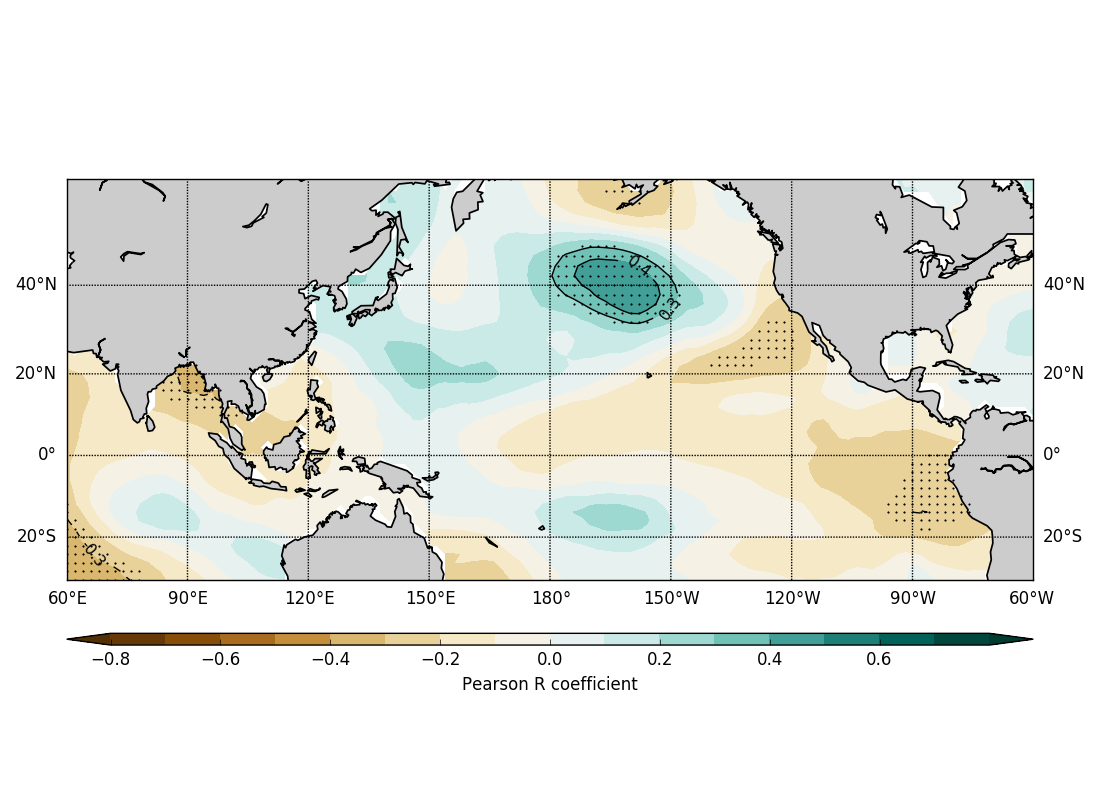
\includegraphics[width=2.6in]{Y:/Code_Data/Chapter1/Plots_new/Corr_maps_final/count/inp_int/sst/sst_curr_JJASO&countJJASOplusinp_intcorr_total.png}}
	\subfloat[ACE:all]{\includegraphics[width=2.6in]{Y:/Code_Data/Chapter1/Plots_new/Corr_maps_final/ACE/inpoly/sst/sst_curr_JJASO&ACEJJASOallcatsinpolycorr_total.png}}
	\subfloat[Count:all]{\includegraphics[width=2.6in]{Y:/Code_Data/Chapter1/Plots_new/Corr_maps_final/count/inp_int/sst/sst_curr_JJASO&countJJASOallcatsinp_intcorr_total.png}}
	
	\caption{SST-JJASO correlated with (1) and ACE and (2) count over the period 1958-2014. a) Low (tropical storms and tropical depressions). b) Medium (categories 1,2) c) High (categories 3, 4, 5) d) a. Stippling indicates grid points with significant correlation at the 95th percentile} \label{fig:corr_JJASO} 
\end{figure} 

The correlation maps in column 1 (SST correlated with ACE) are similar to those in column 2 (SST correlated with count), suggesting that the relationship with SST is dominated by frequency of storms rather than intensity.

The plots in figure \ref{fig:corr_JJASO} show that there are notable differences between the relationship with SST and tropical storm activity for different intensity storms. For the low intensity storms, there is an area of significant positive correlation in the Philippine Sea, extending northwards encompassing the East China Sea and eastwards to the east of Japan (figure \ref{fig:corr_JJASO},2a). This in the the region of the Kuroshio currents, where warm water is advected .....The storms during the season pass over this water in the Philippines / East China Sea, to make landfall in the selected domain. When the SST here is anomalously warm, there are an increased number of tropical storms and tropical depressions making landfall here and vice versa.

For the medium intensity storms, there is a significant negative correlation in the central equatorial Pacific (figure \ref{fig:corr_JJASO}b). For the intense storms (figure \ref{fig:corr_JJASO},c), a maximum correlation of between 0.4 and 0.5 is apparent in the northern North Pacific. No regions of significant correlation are observed across all of the different categories.
%There is a negative correlation in the Southern Indian Ocean and South China Sea, and Bay of Bengal as well as eastern equatorial Pacific. 
The negative correlations in the medium and intense storms in the equatorial Pacific are likely to be El Nino, which varies on an interannual time scale. In both cases, the correlation is negative, suggesting that during El Nino (central for medium and EPAC for intense), there are fewer storms making landfall in the selected domain.

Figures 1d and 2d are the relationship with all storms. The largest area of significance is the equatorial Pacific, with a negative correlation. As might be expected, these plots (1d and 2d) show the largest difference, as there are more storms in total being analysed in these plots and ...
Future correlation maps will show the relationship with count, as the observations are subject to less error than wind that goes into the ACE calculation.
%When the sum of ACE for all categories is plotted as above (not shown), .........


\begin{figure}
	\centering
	\noindent\includegraphics[width=24pc,angle=0]{H:/Documents/Thesis/phd-thesis-template-2.2.2_AC/phd-thesis-template-2.2.2/Figs/ocean_currents2_cut.png}
	\caption{Ocean currents showing Kurushio. Source: \citep{kuroshio}}\label{fig:kuroshio}
\end{figure}


\begin{figure}
	\centering
	%\subfloat[1a]{\includegraphics[width=2.4in]{Y:/Code_Data/Chapter1/Plots_new/Corr_maps/ACE/inpoly/prev_sst_JFM&ACEJJASO63inpolycorr_train.png}} 
	\subfloat[2a]{\includegraphics[width=2.6in]{Y:/Code_Data/Chapter1/Plots_new/Corr_maps_final/count/inp_int/sst/sst_prev_JFM&countJJASO63inp_intcorr_total.png}}
	%\subfloat[1b]{\includegraphics[width=2.4in]{Y:/Code_Data/Chapter1/Plots_new/Corr_maps/ACE/inpoly/prev_sst_JFM&ACEJJASO95inpolycorr_train.png}}
	\subfloat[2a]{\includegraphics[width=2.6in]{Y:/Code_Data/Chapter1/Plots_new/Corr_maps_final/count/inp_int/sst/sst_prev_JFM&countJJASO95inp_intcorr_total.png}}
	%\subfloat[1c]{\includegraphics[width=2.4in]{Y:/Code_Data/Chapter1/Plots_new/Corr_maps/ACE/inpoly/prev_sst_JFM&ACEJJASOplusinpolycorr_train.png}}
	\subfloat[2a]{\includegraphics[width=2.6in]{Y:/Code_Data/Chapter1/Plots_new/Corr_maps_final/count/inp_int/sst/sst_prev_JFM&countJJASOplusinp_intcorr_total.png}}
	%\subfloat[1d]{\includegraphics[width=2.4in]{Y:/Code_Data/Chapter1/Plots_new/Corr_maps/ACE/inpoly/prev_sst_JFM&ACEJJASOallcatsinpolycorr_train.png}}
	\subfloat[2a]{\includegraphics[width=2.6in]{Y:/Code_Data/Chapter1/Plots_new/Corr_maps_final/count/inp_int/sst/sst_prev_JFM&countJJASOallcatsinp_intcorr_total.png}}
	\caption{SST-JFM-1 correlated with count over the period 1958-2014. a) Low (tropical storms and tropical depressions). b) Medium (categories 1,2) c) High (categories 3, 4, 5) d) All storms. Stippling indicates grid points with significant correlation at the 95th percentile} \label{fig:corr_prevJFM} 
\end{figure} 

When correlating ACE-JJASO and count-JJASO with SSTs in the year prior to the storm season, the most consistent and significant signal is seen in JFM ('JFM-1') off the east coast of mainland China, in the East China Sea (figure \ref{fig:corr_prevJFM}) and in the Bay of Bengal (particularly when correlating against count), parts significant in the South China Sea. There is a striking anti-correlation between the results for the low intensity storms (figure \ref{fig:corr_prevJFM}, a) and the high intensity storms (figure \ref{fig:corr_prevJFM}, c) in this region. For the weakest storms, there is a positive correlation with SST, but for the most intense storm this correlation is negative. Both categories show significance at the 95th percentile in this region.  Alongside this region, there are correlations of the opposite sign extending northeastwards towards the Aleutian Islands and also at around 10-20N and to the east of this main site.

The lag between these anomalies and the storm activity is approximately 18 months.

For the medium intensity storms, however, there is no significant correlation with SST in this region (figure \ref{fig:corr_prevJFM}, b). %The highest Pearson R correlation value is around 0.5, giving an R\textsuperscript{2} of 0.25. This suggests that 25\% of the variability in ACE or count each year is explained by the SST in this region in the previous JFM. 

The low intensity storms also have a large region of positive correlation in the eastern equatorial Pacific. During JFM, if there is an El Nino situation, the anomalous sea surface temperature in this region can still be large and decreasing? This indicates that in the year following an El Nino i.e. 15 months later?, there are increased number of tropical storms and depressions in the domain.


%correlated because trend and sst and ace both increasing? or because time series variability is correlated on interannual timescale?
%pLOT storms that do not intersect and see how they miss the domain - above or below or stay out at sea?

In the JFM just before the JJASO season, the signal in this region for the intense storms has largely disappeared although some significance re3mains in the Bay of Bengal for the weak storms. (not shown).

%\begin{figure}
%	\centering
%	\subfloat[2a]{\includegraphics[width=2.6in]{Y:/Code_Data/Chapter1/Plots_new/Corr_maps_final/count/inp_int/sst/sst_curr_JFM&countJJASO63inp_intcorr_total.png}}
%%	\subfloat[2b]{\includegraphics[width=2.4in]{Y:/Code_Data/Chapter1/Plots_new/Corr_maps/count/inp_int/curr_sst_JFM&countJJASO95inp_intcorr_train.png}}
%	\subfloat[2a]{\includegraphics[width=2.6in]{Y:/Code_Data/Chapter1/Plots_new/Corr_maps_final/count/inp_int/sst/sst_curr_JFM&countJJASOplusinp_intcorr_total.png}}
%	
%	\caption{SST-JFM correlated with count-JJASO for within the domain over the training period 1958-2007. a. Tropical storms and tropical depressions. b. Categories 3, 4 and 5. Stippling shows grid points with significant correlation at 95th percentile} \label{fig:corr_currJFM} 
%	\end{figure} 

\begin{table}[h]
	\caption{Coordinates of regions}\label{tregion_coors}
	\begin{center}
		\begin{tabular}{ccc}
			\hline\hline
			Region & Coordinates & Signal\\
			\hline
			East China Sea & 0-40N, 120-140E,  & JJASO, Low, positive  \\ 
			East China Sea2 & 15-35N, 120-140E,  & JFM-1, low, positive. JFM-1, high, negative \\ 
			Bay of Bengal & 5-20N, 80-100E & JJASO, high, negative. JFM-1, low, positive. JFM-1, high, positive \\ 
			NNPac & 32-47N, 180-150W & JJASO, high, positive  \\ 
			Kuroshio & 35-47N, 145-175E & JJASO, Low, positive, JFM-1, low, negative. JFM-1, high, positive  \\ 
			Oyashio & 40-53N, 155-170E & JFM-1, low, negative. JFM-1, high, positive  \\
			Anew & 10-20N, 160-180E & JFM-1, low, negative. JFM-1, high, positive   \\ 
						
			\hline
		\end{tabular}
	\end{center}
\end{table}


This region of interest will be further examined, concentrating on the weak and intense storms only.

Figure \ref {fig:SCS} shows the domain where these opposing strong correlations are apparent. 
\begin{figure} % remove [h] and this appeared in the correct place
	\noindent\includegraphics[width=26pc,angle=0]{Y:/Code_Data/Chapter1/Plots_new/Maps/corr_regions.png}
	\caption{Regions of high correlations}\label{fig:SCS}
\end{figure}

\begin{figure} % remove [h] and this appeared in the correct place
	\noindent\includegraphics[width=26pc,angle=0]{Y:/Code_Data/Chapter1/Plots_new/Maps/nino_regions.png}
	\caption{Nino regions}\label{fig:nino}
\end{figure}

% check means are 50 years or 57 years?
Figure \ref{fig:SST_JJASO} shows that during the tropical cyclone season (JJASO), there is a large region of warm SSTs, well above the 26.5$^0$C proposed threshold for genesis (section \ref{ocean}). The standard deviation of the SSTs across the period in both JJASO and JFM shows the most variation year to year in the equatorial Pacific, where the El Nino phenomenon has a signal and this shows significant interannual variability. %Off the east coast of Asia and into the Bay of Bengal, the standard deviation is 0.6 to 0.3 C??

\begin{figure} % remove [h] and this appeared in the correct place
	\subfloat[a]{\includegraphics[width=3.5in]{Y:/Code_Data/Chapter1/Plots_new/Charts/sst_JJASO_mean.png}} 
	\subfloat[b]{\includegraphics[width=3.5in]{Y:/Code_Data/Chapter1/Plots_new/Charts/sst_JJASO_std.png}} 
	\subfloat[c]{\includegraphics[width=3.5in]{Y:/Code_Data/Chapter1/Plots_new/Charts/sst_JFM_mean.png}} 
	\subfloat[c]{\includegraphics[width=3.5in]{Y:/Code_Data/Chapter1/Plots_new/Charts/sst_JFM_std.png}} 
	
	\caption{SST climatology. (a) JJASO mean (b) JJASO standard deviation (c) JFM standard deviation. The standard deviations are of the JJASO mean across the 50 year training period.}\label{fig:SST_JJASO}
\end{figure}

Unlike in the North Atlantic, where tropical cyclogenesis is restricted by the cooler SSTs, in the West Pacific, there is a large region where SSTs are not the restricting factor. Therefore, something else at play? Also steering is important.
This region of warm water migrates north or south depending on the season. Warm pool to the west of the basin and cooler upwelling water to the east.

This period examined from 1958 and is likely to contain decadal signals. To assess whether the signals seen in figures \ref{fig:corr_JJASO} and \ref{fig:corr_prevJFM} are stable throughout the period, the results have been broken down into three periods that line up with different Pacific Decadal Oscillation (PDO) phases (cold, warm and mixed) (figure \ref{fig:PDO_time}, table \ref{tperiods}).

% 	\begin{figure}
% 		\noindent\includegraphics[width=35pc,angle=0]{Y:/Code_Data/PDO/Figure_PDO-01.jpg}\\
% 		\caption{The Pacific Decadal Oscillation( (PDO) Index. From https://www.nwfsc.noaa.gov/research}\label{fig:PDO_time}
% 	\end{figure}


\begin{figure}
	\centering
	\noindent\includegraphics[width=20pc,angle=0]{Y:/Code_Data/Chapter1/Plots_new/Charts/PDO_5814_filled.png}
	\caption{The Pacific Decadal Oscillation Index}\label{fig:PDO_time}
\end{figure}

\begin{table}[h]
	\caption{Periods}\label{tperiods}
	\begin{center}
		\begin{tabular}{ccc}
			\hline\hline
			Years & Number of years & PDO state \\
			\hline
			1958-1975 & 18 & cold  \\ 
			1976-1997 & 22 & warm  \\ 
			1998-2014 & 17 & mixed  \\ 
			
			\hline
		\end{tabular}
	\end{center}
\end{table}


The following figures show the correlation maps for each category for the three different periods \ref{tperiods}. Column 1 is 1958-1975 (cold), 2 is 1976-1997 (warm), and 3 is 1998-2014 (mixed). 


\begin{figure}
	\centering
	
	\subfloat[2a]{\includegraphics[width=1.8in]{Y:/Code_Data/Chapter1/Plots_new/Corr_maps_final/count/inp_int/sst/sst_curr_JJASO&countJJASO63inp_intcorr_early.png}}
	\subfloat[2a]{\includegraphics[width=1.8in]{Y:/Code_Data/Chapter1/Plots_new/Corr_maps_final/count/inp_int/sst/sst_curr_JJASO&countJJASO63inp_intcorr_mid.png}}
	\subfloat[2a]{\includegraphics[width=1.8in]{Y:/Code_Data/Chapter1/Plots_new/Corr_maps_final/count/inp_int/sst/sst_curr_JJASO&countJJASO63inp_intcorr_late.png}}
	
%	\subfloat[2a]{\includegraphics[width=1.8in]{Y:/Code_Data/Chapter1/Plots_new/Corr_maps_final/count/inp_int/sst/sst_curr_JJASO&countJJASO95inp_intcorr_early.png}}
%	\subfloat[2a]{\includegraphics[width=1.8in]{Y:/Code_Data/Chapter1/Plots_new/Corr_maps_final/count/inp_int/sst/sst_curr_JJASO&countJJASO95inp_intcorr_mid.png}}
%	\subfloat[2a]{\includegraphics[width=1.8in]{Y:/Code_Data/Chapter1/Plots_new/Corr_maps_final/count/inp_int/sst/sst_curr_JJASO&countJJASO95inp_intcorr_late.png}}
	
	\subfloat[2a]{\includegraphics[width=1.8in]{Y:/Code_Data/Chapter1/Plots_new/Corr_maps_final/count/inp_int/sst/sst_curr_JJASO&countJJASOplusinp_intcorr_early.png}}
	\subfloat[2a]{\includegraphics[width=1.8in]{Y:/Code_Data/Chapter1/Plots_new/Corr_maps_final/count/inp_int/sst/sst_curr_JJASO&countJJASOplusinp_intcorr_mid.png}}
	\subfloat[2a]{\includegraphics[width=1.8in]{Y:/Code_Data/Chapter1/Plots_new/Corr_maps_final/count/inp_int/sst/sst_curr_JJASO&countJJASOplusinp_intcorr_late.png}}
	\caption{SST-JJASO correlated with count-JJASO for within the domain for 1958-1975 (1), 1976-1997 (2), 1998-2014 (3). a. Tropical storms and tropical depressions. b. Categories 1,2 c. Categories 3, 4, 5.  Stippling shows grid points with significant correlation at 95th percentile} \label{fig:corr_JJASO_periods} 
\end{figure} 

sort this out:

In JJASO, the positive correlation seen to the east of Japan is strong in the middle (warm period), with no significant correlations in the other periods. The positive correlation in the Philippine Sea and East China Sea are present in less coherent regions and not as strong a correlation (figure \ref{fig:corr_JJASO_periods}, 2a). The final (mixed) phase has no areas of significant correlation. 
 There are also areas of significant correlation across the equatorial Pacific  -check.

For the high intensity storms, the positive correlation at approximately 160W and 40N is apparent in all periods, strongest during the cool phase when it has a dipole with the Kuroshio region. (refer to PDO phase diagram in intro).
%cHECK WHETHER PDO YEARS SHOULD BE ADJUSTED BY ONE WHEN LOOKING AT PREV YEAR

\begin{figure}
	\centering
	
	\subfloat[2a]{\includegraphics[width=1.8in]{Y:/Code_Data/Chapter1/Plots_new/Corr_maps_final/count/inp_int/sst/sst_prev_JFM&countJJASO63inp_intcorr_early.png}}
	\subfloat[2a]{\includegraphics[width=1.8in]{Y:/Code_Data/Chapter1/Plots_new/Corr_maps_final/count/inp_int/sst/sst_prev_JFM&countJJASO63inp_intcorr_mid.png}}
	\subfloat[2a]{\includegraphics[width=1.8in]{Y:/Code_Data/Chapter1/Plots_new/Corr_maps_final/count/inp_int/sst/sst_prev_JFM&countJJASO63inp_intcorr_late.png}}
	
	\subfloat[2a]{\includegraphics[width=1.8in]{Y:/Code_Data/Chapter1/Plots_new/Corr_maps_final/count/inp_int/sst/sst_prev_JFM&countJJASO95inp_intcorr_early.png}}
	\subfloat[2a]{\includegraphics[width=1.8in]{Y:/Code_Data/Chapter1/Plots_new/Corr_maps_final/count/inp_int/sst/sst_prev_JFM&countJJASO95inp_intcorr_mid.png}}
	\subfloat[2a]{\includegraphics[width=1.8in]{Y:/Code_Data/Chapter1/Plots_new/Corr_maps_final/count/inp_int/sst/sst_prev_JFM&countJJASO95inp_intcorr_late.png}}
	
	\subfloat[2a]{\includegraphics[width=1.8in]{Y:/Code_Data/Chapter1/Plots_new/Corr_maps_final/count/inp_int/sst/sst_prev_JFM&countJJASOplusinp_intcorr_early.png}}
	\subfloat[2a]{\includegraphics[width=1.8in]{Y:/Code_Data/Chapter1/Plots_new/Corr_maps_final/count/inp_int/sst/sst_prev_JFM&countJJASOplusinp_intcorr_mid.png}}
	\subfloat[2a]{\includegraphics[width=1.8in]{Y:/Code_Data/Chapter1/Plots_new/Corr_maps_final/count/inp_int/sst/sst_prev_JFM&countJJASOplusinp_intcorr_late.png}}
	\caption{SST-JFM-1 correlated with count-JJASO for within the domain for 1958-1975 (1), 1976-1997 (2), 1998-2014 (3). a. Tropical storms and tropical depressions. b. Categories 1,2 c. Categories 3, 4, 5.  Stippling shows grid points with significant correlation at 95th percentile} \label{fig:corr_prevJFM_periods} 
\end{figure} 

Figure \ref{fig:corr_prevJFM_periods} shows the correlation maps between count-JJASO and SST-JFM-1 broken down into three different periods for the three categories. 
The strong positive correlation off the east coast of China and into the Bay of Bengal is dominated by the early period (cold PDO), for both the weak storms (1a) and intense storms (1c). For the weak storms, the negative correlation to the east of this region at 10-20N remains, although the positive signal is not apparent. During the mixed phase, there is a region of signficant positive correlation in the East China Sea, although this is slightly weaker than the mean over the period and no signal in the Bay of Bengal.
For the strong storms, during the warm period and mixed period, there are no significant correlations in the region of interest, although in the mixed period, the opposing correlation to the east of the region is shown.



It is not only the sea surface that affects tropical storm activity, but the deeper ocean can have an influence (ref section). Therefore the ocean heat content (OHC) (to 100m?) is also investigated.

\begin{figure} % remove [h] and this appeared in the correct place
	\centering
	\noindent\includegraphics[width=30pc,angle=0]{Y:/Code_Data/Chapter1/Plots_new/Charts/ohc_JJASO_mean.png}
	%	\noindent\includegraphics[width=30pc,angle=0]{Y:/Code_Data/Chapter1/Plots_new/Charts/ohc_JJASO_std.png}\\
	\caption{OHC (to 100 m) mean during JJASO}\label{fig:OHC_JJASO}
\end{figure}

The mean OHC to 100m during the JJASO season shows a very similar pattern to SST (figure \ref{fig:OHC_JJASO}), with an area of relatively warm water extending from the tropics to approximately 30N. Water in the west of the basin is warmer than the east, where there is upwelling of cooler water.


Figure \ref{fig:ohc_currJJASO} shows the correlations with OHC-JJASO and count-JJASO.

\begin{figure}
	\centering

	\subfloat[2a]{\includegraphics[width=2.6in]{Y:/Code_Data/Chapter1/Plots_new/Corr_maps_final/count/inp_int/ohc/ohc_curr_JJASO&countJJASO63inp_intcorr_total.png}}
%	\subfloat[2a]{\includegraphics[width=2.6in]{Y:/Code_Data/Chapter1/Plots_new/Corr_maps_final/count/inp_int/ohc/ohc_curr_JJASO&countJJASO95inp_intcorr_total.png}}
	\subfloat[2a]{\includegraphics[width=2.6in]{Y:/Code_Data/Chapter1/Plots_new/Corr_maps_final/count/inp_int/ohc/ohc_curr_JJASO&countJJASOplusinp_intcorr_total.png}}
%	\subfloat[2a]{\includegraphics[width=2.6in]{Y:/Code_Data/Chapter1/Plots_new/Corr_maps_final/count/inp_int/ohc/ohc_curr_JJASO&countJJASOallcatsinp_intcorr_total.png}}
	\caption{OHC-JJASO correlated with count-JJASO for within the domain over the training period 1958-2007. a. Tropical storms and tropical depressions. b. Categories 1,2 c. Categories 3, 4, 5. Stippling shows grid points with significant correlation at 95th percentile} \label{fig:ohc_currJJASO} 
\end{figure} 

Ocean heat content (OHC) (to 100 m) was also analysed in the same method as above. Data is at twice the resolution of SST (1 rather than 2 degrees) and so more detail in spatial patterns is apparent. 
The positive correlations in the Philippines Sea, East China Sea and along the Kuroshio current are not as clear in OHC as with SST, although there are some stippled grid points, especially close to the east coast of the mainland.

%Correlation maps show a very similar relationship with ACE and frequency as the SST (figure \ref{fig:corr_JJASO}), although are at twice the resolution. During the storm season, the OHC show some significant negative correlation in the eastern equatorial Pacific, not present in the SST maps, and does not show the positive significant areas off the east coast of Asia and in the vicinity of Japan. 

The positive correlation in the northern Pacific is present in SST and OHC (figures) for the intense storms, with a more strongly negative correlation below this.

OHC-JFM-1 shows the opposing correlations for weak and intense storms in the East China Sea, although this is less extensive and does not extend into the Bay of Bengal and towards the Aleutian Islands.

\begin{figure}
	\centering
	
	\subfloat[2a]{\includegraphics[width=2.6in]{Y:/Code_Data/Chapter1/Plots_new/Corr_maps_final/count/inp_int/ohc/ohc_prev_JFM&countJJASO63inp_intcorr_total.png}}

	\subfloat[2a]{\includegraphics[width=2.6in]{Y:/Code_Data/Chapter1/Plots_new/Corr_maps_final/count/inp_int/ohc/ohc_prev_JFM&countJJASOplusinp_intcorr_total.png}}

	\caption{OHC-JFM-1 correlated with count-JJASO for within the domain over the training period 1958-2007. a. Tropical storms and tropical depressions. b. Categories 1,2 c. Categories 3, 4, 5. Stippling shows grid points with significant correlation at 95th percentile} \label{fig:ohc_prevJFM} 
\end{figure} 

As well as these oceanic variables, a number of atmospheric variables were analysed using the JRA-55 reanalysis data.
% Examine if there is an atmospheric pattern related to the ACE or count in JJASO. Same correlation plots, but with mslp, geopotential height, ]
%With mslp and geopotential check out monsoon trough, subtropical high

\subsubsection{Atmospheric variables}

The ocean and atmosphere interact through the marine boundary layer (MBL) and likely that signals are...

\begin{figure}
	\centering
	%	\subfloat[1a]{\includegraphics[width=2.4in]{Y:/Code_Data/Chapter1/Plots_new/Corr_maps/ACE/inpoly/curr_sst_JJASO&ACEJJASO63inpolycorr_trainmslp.png}} 
	\subfloat[2a]{\includegraphics[width=2.6in]{Y:/Code_Data/Chapter1/Plots_new/Corr_maps_final/count/inp_int/mslp/mslp_curr_JJASO&countJJASO63inp_intcorr_total.png}}
	\subfloat[2a]{\includegraphics[width=2.6in]{Y:/Code_Data/Chapter1/Plots_new/Corr_maps_final/count/inp_int/geop/geop_curr_JJASO&countJJASO63inp_intcorr_total.png}}
	%\subfloat[1b]{\includegraphics[width=2.4in]{Y:/Code_Data/Chapter1/Plots_new/Corr_maps/ACE/inpoly/curr_sst_JJASO&ACEJJASO95inpolycorr_trainmslp.png}}
%	\subfloat[2a]{\includegraphics[width=2.6in]{Y:/Code_Data/Chapter1/Plots_new/Corr_maps_final/count/inp_int/mslp/mslp_curr_JJASO&countJJASO95inp_intcorr_total.png}}
%	\subfloat[2a]{\includegraphics[width=2.6in]{Y:/Code_Data/Chapter1/Plots_new/Corr_maps_final/count/inp_int/geop/geop_curr_JJASO&countJJASO95inp_intcorr_total.png}}
	%\subfloat[1c]{\includegraphics[width=2.4in]{Y:/Code_Data/Chapter1/Plots_new/Corr_maps/ACE/inpoly/curr_sst_JJASO&ACEJJASOplusinpolycorr_trainmslp.png}}
	\subfloat[2a]{\includegraphics[width=2.6in]{Y:/Code_Data/Chapter1/Plots_new/Corr_maps_final/count/inp_int/mslp/mslp_curr_JJASO&countJJASOplusinp_intcorr_total.png}}
	\subfloat[2a]{\includegraphics[width=2.6in]{Y:/Code_Data/Chapter1/Plots_new/Corr_maps_final/count/inp_int/geop/geop_curr_JJASO&countJJASOplusinp_intcorr_total.png}}
	
%	\subfloat[2a]{\includegraphics[width=2.6in]{Y:/Code_Data/Chapter1/Plots_new/Corr_maps_final/count/inp_int/mslp/mslp_curr_JJASO&countJJASOallcatsinp_intcorr_total.png}}
%	\subfloat[2d]{\includegraphics[width=2.4in]{Y:/Code_Data/Chapter1/Plots_new/Corr_maps/count/inp_int/curr_sst_JJASO&countJJASOallcatsinp_intcorr_traingeop.png}}	
	\caption{MSLP-JJASO and geop500-JJASO correlated with count-JJASO for within the domain over the training period 1958-2007. a. Tropical storms and tropical depressions. b. Categories 1,2 c. Categories 3, 4, 5. Stippling shows grid points with significant correlation at 95th percentile} \label{fig:corr_curr_JJASO_mslpgeop} 
\end{figure} 

%\begin{figure}
%	\centering
%	%	\subfloat[1a]{\includegraphics[width=2.4in]{Y:/Code_Data/Chapter1/Plots_new/Corr_maps/ACE/inpoly/curr_sst_JJASO&ACEJJASO63inpolycorr_trainmslp.png}} 
%	\subfloat[2a]{\includegraphics[width=2.4in]{Y:/Code_Data/Chapter1/Plots_new/Corr_maps/count/inp_int/curr_sst_JJASO&countJJASO63inp_intcorr_traingeop.png}}
%	%\subfloat[1b]{\includegraphics[width=2.4in]{Y:/Code_Data/Chapter1/Plots_new/Corr_maps/ACE/inpoly/curr_sst_JJASO&ACEJJASO95inpolycorr_trainmslp.png}}
%	\subfloat[2b]{\includegraphics[width=2.4in]{Y:/Code_Data/Chapter1/Plots_new/Corr_maps/count/inp_int/curr_sst_JJASO&countJJASO95inp_intcorr_traingeop.png}}
%	%\subfloat[1c]{\includegraphics[width=2.4in]{Y:/Code_Data/Chapter1/Plots_new/Corr_maps/ACE/inpoly/curr_sst_JJASO&ACEJJASOplusinpolycorr_trainmslp.png}}
%	\subfloat[2c]{\includegraphics[width=2.4in]{Y:/Code_Data/Chapter1/Plots_new/Corr_maps/count/inp_int/curr_sst_JJASO&countJJASOplusinp_intcorr_traingeop.png}}
%	\caption{geopotential(500)-JJASO correlated with count-JJASO for within the domain over the training period 1958-2007. a. Tropical storms and tropical depressions. b. Categories 1,2 c. Categories 3, 4, 5. Stippling shows grid points with significant correlation at 95th percentile} \label{fig:corr_curr_JJASO_geop} 
%\end{figure} 
Tie these atm results into sst results

Mean sea level pressure (mslp) and 500 hPa geopotential height are correlated with count-JJASO (figure \ref{fig:corr_curr_JJASO_mslpgeop}). The patterns are almost identical.

For the low intensity storms, there is an area of significant correlation in the East China Sea and South China Sea, which is at the same location as the significant positive SST signal. When mslp is anomalously high (and SST anomalously low), there is a decrease in the frequency of low intensity storms making landfall in the domain. There is a positive correlation with mslp in parts of Alaska and the northeast coast of the USA.
For the high intensity storms, there is a region of signficant positive correlation in the northern North Pacific, although this is shifted to the north and is weaker and smaller.


Figure \ref{fig:mslp_JJASO} shows the mean mslp during JJASO, and the subtropical high is clearly visible, centred off the west coast of the USA and extending westwards towards Asia. The mslp during JJASO / all year? across the mid and high latitudes is more variable year to year than across the Tropics.

\begin{figure} % remove [h] and this appeared in the correct place

	\subfloat[a]{\includegraphics[width=3.5in]{Y:/Code_Data/Chapter1/Plots_new/Charts/mslp_JJASO_mean.png}} 
	\subfloat[b]{\includegraphics[width=3.5in]{Y:/Code_Data/Chapter1/Plots_new/Charts/mslp_JJASO_std.png}} 
	\subfloat[c]{\includegraphics[width=3.5in]{Y:/Code_Data/Chapter1/Plots_new/Charts/mslp_JFM_mean.png}} 
	\subfloat[d]{\includegraphics[width=3.5in]{Y:/Code_Data/Chapter1/Plots_new/Charts/mslp_JFM_std.png}} 
	
	\caption{MSLP climatology (a) mean and (b) standard deviation during the JJASO season}\label{fig:mslp_JJASO}
\end{figure}


In JFM-1, there are no strong correlations over the region of SST. However, there are opposing correlations running north to south down China, although only significant for the intense storms. There are large regions of positive SST over the ocean for the weak storms, notably in the Indian Ocean.


\begin{figure}
	\centering
%	\subfloat[2a]{\includegraphics[width=2.6in]{Y:/Code_Data/Chapter1/Plots_new/Corr_maps_final/ACE/inpoly/mslp/mslp_prev_JFM&ACEJJASO63inpolycorr_total.png}}
	\subfloat[2a]{\includegraphics[width=2.6in]{Y:/Code_Data/Chapter1/Plots_new/Corr_maps_final/count/inp_int/mslp/mslp_prev_JFM&countJJASO63inp_intcorr_total.png}}
%	\subfloat[2a]{\includegraphics[width=2.6in]{Y:/Code_Data/Chapter1/Plots_new/Corr_maps_final/ACE/inpoly/mslp/mslp_prev_JFM&ACEJJASO95inpolycorr_total.png}}
%	\subfloat[2a]{\includegraphics[width=2.6in]{Y:/Code_Data/Chapter1/Plots_new/Corr_maps_final/count/inp_int/mslp/mslp_prev_JFM&countJJASO95inp_intcorr_total.png}}
%	\subfloat[2a]{\includegraphics[width=2.6in]{Y:/Code_Data/Chapter1/Plots_new/Corr_maps_final/ACE/inpoly/mslp/mslp_prev_JFM&ACEJJASOplusinpolycorr_total.png}}
	\subfloat[2a]{\includegraphics[width=2.6in]{Y:/Code_Data/Chapter1/Plots_new/Corr_maps_final/count/inp_int/mslp/mslp_prev_JFM&countJJASOplusinp_intcorr_total.png}}
%	\subfloat[2a]{\includegraphics[width=2.6in]{Y:/Code_Data/Chapter1/Plots_new/Corr_maps_final/ACE/inpoly/mslp/mslp_prev_JFM&ACEJJASOallcatsinpolycorr_total.png}}
%	\subfloat[2a]{\includegraphics[width=2.6in]{Y:/Code_Data/Chapter1/Plots_new/Corr_maps_final/count/inp_int/mslp/mslp_prev_JFM&countJJASOallcatsinp_intcorr_total.png}}
	
	\caption{MSLP-JFM-1 correlated with count-JJASO for within the domain over the training period 1958-2007. a. Tropical storms and tropical depressions. b. Categories 1,2 c. Categories 3, 4, 5. Stippling shows grid points with significant correlation at 95th percentile} \label{fig:corr_prevJFM_mslp} 
\end{figure} 

Geopotential height is good for the mid-latitudes. In the Tropics, pressure fields and geopotential are flat because of a weak Coriolis. Look at winds in Tropics. Because not constrained by geostrophy in Tropics.

The zonal wind has an opposing relationship with frequency between low and high in a region upstream of landfall.
The winds are examined at 500 hPa and 850 hPa. 
During JJASO, there is no strong correlation where the SST signal was in the Philippine Sea and East China Sea, but there is a significant negative correlation along the Kuroshio, where a correlation was seen in the weak storms. Relate to SST anomaly. Also for the weak storms, an area approximately 20 degrees (2000 km) to the east of landfall is significant positive correlation. When there is anomalous westerly winds (or reduced easterlies), there is an increased frequency of weak storms. In a similar location, to the east of the landfall domain, there is a negative correlation for the intense storms. When the wind is anomalously easterly (ie reduced u wind), there is an increased frequency of intense storms making landfall in the region.


\begin{figure}
	\centering
	\subfloat[2a]{\includegraphics[width=2.6in]{Y:/Code_Data/Chapter1/Plots_new/Corr_maps_final/count/inp_int/u500/u500_curr_JJASO&countJJASO63inp_intcorr_total.png}}
	\subfloat[2a]{\includegraphics[width=2.6in]{Y:/Code_Data/Chapter1/Plots_new/Corr_maps_final/count/inp_int/u850/u850_curr_JJASO&countJJASO63inp_intcorr_total.png}}		%\subfloat[2a]{\includegraphics[width=2.6in]{Y:/Code_Data/Chapter1/Plots_new/Corr_maps_final/count/inp_int/u500/u500_curr_JJASO&countJJASO95inp_intcorr_total.png}}
	%\subfloat[2b]{\includegraphics[width=2.4in]{Y:/Code_Data/Chapter1/Plots_new/Corr_maps/count/inp_int/curr_sst_JJASO&countJJASO95inp_intcorr_trainu850.png}}		\subfloat[2a]{\includegraphics[width=2.6in]{Y:/Code_Data/Chapter1/Plots_new/Corr_maps_final/count/inp_int/u500/u500_curr_JJASO&countJJASOplusinp_intcorr_total.png}}
	\subfloat[2a]{\includegraphics[width=2.6in]{Y:/Code_Data/Chapter1/Plots_new/Corr_maps_final/count/inp_int/u500/u500_curr_JJASO&countJJASOplusinp_intcorr_total.png}}
	\subfloat[2a]{\includegraphics[width=2.6in]{Y:/Code_Data/Chapter1/Plots_new/Corr_maps_final/count/inp_int/u850/u850_curr_JJASO&countJJASOplusinp_intcorr_total.png}}
%	\subfloat[2a]{\includegraphics[width=2.6in]{Y:/Code_Data/Chapter1/Plots_new/Corr_maps_final/count/inp_int/u500/u500_curr_JJASO&countJJASOallcatsinp_intcorr_total.png}}
%	\subfloat[2c]{\includegraphics[width=2.4in]{Y:/Code_Data/Chapter1/Plots_new/Corr_maps/count/inp_int/curr_sst_JJASO&countJJASOallcatsinp_intcorr_trainu850.png}}

	\caption{u-JJASO correlated with count-JJASO for within the domain over the training period 1958-2007.(1) u500, (2) u850. a. Tropical storms and tropical depressions. b. Categories 1,2 c. Categories 3, 4, 5. Stippling shows grid points with significant correlation at 95th percentile} \label{fig:corr_curr_JJASO_u} 
\end{figure} 





\begin{figure}
	\centering
	\subfloat[2a]{\includegraphics[width=2.6in]{Y:/Code_Data/Chapter1/Plots_new/Corr_maps_final/count/inp_int/u500/u500_prev_JFM&countJJASO63inp_intcorr_total.png}}
	\subfloat[2a]{\includegraphics[width=2.6in]{Y:/Code_Data/Chapter1/Plots_new/Corr_maps_final/count/inp_int/u850/u850_prev_JFM&countJJASO63inp_intcorr_total.png}}	%\subfloat[2a]{\includegraphics[width=2.6in]{Y:/Code_Data/Chapter1/Plots_new/Corr_maps_final/count/inp_int/u500/u500_prev_JFM&countJJASO95inp_intcorr_total.png}}
%	\subfloat[2b]{\includegraphics[width=2.4in]{Y:/Code_Data/Chapter1/Plots_new/Corr_maps/count/inp_int/prev_sst_JFM&countJJASO95inp_intcorr_trainu850.png}}		\subfloat[2a]{\includegraphics[width=2.6in]{Y:/Code_Data/Chapter1/Plots_new/Corr_maps_final/count/inp_int/u500/u500_prev_JFM&countJJASOplusinp_intcorr_total.png}}
	\subfloat[2a]{\includegraphics[width=2.6in]{Y:/Code_Data/Chapter1/Plots_new/Corr_maps_final/count/inp_int/u500/u500_prev_JFM&countJJASOplusinp_intcorr_total.png}}		\subfloat[2a]{\includegraphics[width=2.6in]{Y:/Code_Data/Chapter1/Plots_new/Corr_maps_final/count/inp_int/u850/u850_prev_JFM&countJJASOplusinp_intcorr_total.png}}
%	\subfloat[2a]{\includegraphics[width=2.6in]{Y:/Code_Data/Chapter1/Plots_new/Corr_maps_final/count/inp_int/u500/u500_prev_JFM&countJJASOallcatsinp_intcorr_total.png}}
%	\subfloat[2c]{\includegraphics[width=2.4in]{Y:/Code_Data/Chapter1/Plots_new/Corr_maps/count/inp_int/prev_sst_JFM&countJJASOallcatsinp_intcorr_trainu850.png}}
	\caption{u-JFM-1 correlated with count-JJASO for within the domain over the training period 1958-2007.(1) u500, (2) u850. a. Tropical storms and tropical depressions. b. Categories 1,2 c. Categories 3, 4, 5. Stippling shows grid points with significant correlation at 95th percentile} \label{fig:corr_prevJFM_u} 
\end{figure} 

Temp JJASO shows same SST patterns with nothing interesting over land. No need to show it.

%\begin{figure}
%	\centering
%	\subfloat[2a]{\includegraphics[width=2.6in]{Y:/Code_Data/Chapter1/Plots_new/Corr_maps_final/count/inp_int/temp1000/temp1000_curr_JJASO&countJJASO63inp_intcorr_total.png}}
%	\subfloat[2a]{\includegraphics[width=2.6in]{Y:/Code_Data/Chapter1/Plots_new/Corr_maps_final/count/inp_int/temp850/temp850_curr_JJASO&countJJASO63inp_intcorr_total.png}}	
%	\subfloat[2a]{\includegraphics[width=2.6in]{Y:/Code_Data/Chapter1/Plots_new/Corr_maps_final/count/inp_int/temp1000/temp1000_curr_JJASO&countJJASOplusinp_intcorr_total.png}}
%	\subfloat[2a]{\includegraphics[width=2.6in]{Y:/Code_Data/Chapter1/Plots_new/Corr_maps_final/count/inp_int/temp850/temp850_curr_JJASO&countJJASOplusinp_intcorr_total.png}}	
%	\caption{Temp1000-JJASO correlated with count-JJASO for within the domain over the training period 1958-2007. a. Tropical storms and tropical depressions. b. Categories 1,2 c. Categories 3, 4, 5. Stippling shows grid points with significant correlation at 95th percentile} \label{fig:corr_JJASO_temp} 
%\end{figure} 

Temperature at 1000 hPa shows the same opposing significant relationships for the weak and intense storms in the South China Sea as seen with SST. This field gives additional information over land and also shows that this relationship extends onto land a couple of hundred kilometres. Point of showing temp is that anomaly extends onto land.

\begin{figure}
	\centering
	\subfloat[2a]{\includegraphics[width=2.6in]{Y:/Code_Data/Chapter1/Plots_new/Corr_maps_final/count/inp_int/temp1000/temp1000_prev_JFM&countJJASO63inp_intcorr_total.png}}
	\subfloat[2a]{\includegraphics[width=2.6in]{Y:/Code_Data/Chapter1/Plots_new/Corr_maps_final/count/inp_int/temp850/temp850_prev_JFM&countJJASO63inp_intcorr_total.png}}	%\subfloat[2a]{\includegraphics[width=2.6in]{Y:/Code_Data/Chapter1/Plots_new/Corr_maps_final/count/inp_int/temp1000/temp1000_prev_JFM&countJJASO95inp_intcorr_total.png}}
	%\subfloat[2a]{\includegraphics[width=2.6in]{Y:/Code_Data/Chapter1/Plots_new/Corr_maps_final/count/inp_int/temp850/temp850_prev_JFM&countJJASO95inp_intcorr_total.png}}
	\subfloat[2a]{\includegraphics[width=2.6in]{Y:/Code_Data/Chapter1/Plots_new/Corr_maps_final/count/inp_int/temp1000/temp1000_prev_JFM&countJJASOplusinp_intcorr_total.png}}
	\subfloat[2a]{\includegraphics[width=2.6in]{Y:/Code_Data/Chapter1/Plots_new/Corr_maps_final/count/inp_int/temp850/temp850_prev_JFM&countJJASOplusinp_intcorr_total.png}}	%\subfloat[2a]{\includegraphics[width=2.6in]{Y:/Code_Data/Chapter1/Plots_new/Corr_maps_final/count/inp_int/temp1000/temp1000_prev_JFM&countJJASOallcatsinp_intcorr_total.png}}
	%\subfloat[2a]{\includegraphics[width=2.6in]{Y:/Code_Data/Chapter1/Plots_new/Corr_maps_final/count/inp_int/temp850/temp850_prev_JFM&countJJASOallcatsinp_intcorr_total.png}}
	\caption{Temp1000-JFM-1 correlated with count-JJASO for within the domain over the training period 1958-2007. a. Tropical storms and tropical depressions. b. Categories 1,2 c. Categories 3, 4, 5. Stippling shows grid points with significant correlation at 95th percentile} \label{fig:corr_prevJFM_temp} 
\end{figure} 


Ocean forcing the atmosphere vs atmosphere forcing ocean.


In order to examine the cause of these SST anomalies off the east coast, sensible and latent heat flux are examined.
JFM plots - save year, do I see re-emergence? yes!

SST anomalies in winter because driven by atmospheric systems (active). Summer has a shallow mixed layer. Anomalies stay deep. Next winter, mixed up - re-emergence.

\subsubsection{Heat flux}

Heat flux W per m\textsuperscript{2}
Latent heat flux is the flux of heat from the Earth's surface to the atmosphere that is associated with evaporation of water at the surface and subsequent condensation of water vapor in the troposphere. 
From Arnaud 1998 paper
Lag covariance between surface heat flux and SST anomalies, we have shown that the turbulent heat
flux plays a dual forcing and damping role. As discussed in Frankignoul (1985), the heat flux
feedback is dominated by the turbulent heat fluxes (latent and sensible heat flux), and it can be estimated from
the response of atmospheric general circulation models (AGCMs) to prescribed SST anomalies. However, the
relationship between the SST and heat flux anomaly fields may be rather complex and seems model dependent
and, in some cases, a function of the location and polarity the SST anomaly
LHF plots in prev year - lots of significant spots, but moves around each month

\begin{figure}[h]
	\centering
	\noindent\includegraphics[width=26pc,angle=0]{H:/Documents/Thesis/phd-thesis-template-2.2.2_AC/phd-thesis-template-2.2.2/Figs/heat_flux_pic.png}
	\caption{Need to sort out this diagram}\label{fig:heat_flux}
\end{figure}



\begin{figure} % remove [h] and this appeared in the correct place
	
	\subfloat[a]{\includegraphics[width=3.5in]{Y:/Code_Data/Chapter1/Plots_new/Charts/hf_JJASO_mean.png}} 
	\subfloat[b]{\includegraphics[width=3.5in]{Y:/Code_Data/Chapter1/Plots_new/Charts/hf_JJASO_std.png}} 
	\subfloat[c]{\includegraphics[width=3.5in]{Y:/Code_Data/Chapter1/Plots_new/Charts/hf_JFM_mean.png}} 
	\subfloat[d]{\includegraphics[width=3.5in]{Y:/Code_Data/Chapter1/Plots_new/Charts/hf_JFM_std.png}} 
	
	\caption{Heat flux climatology (a) mean and (b) standard deviation during the JJASO season}\label{fig:HF_climat}
\end{figure}


During the JJASO season, mean heat flux (latent plus sensible) is generally consistent across longitude bands, with lower values towards the poles. In the winter (JFM), the largest heat fluxes are dominated in a small region around the Kuroshio current. Which is ... This warm ocean current transfers heat upwards into the relatively cool atmosphere.
Tropics - ocean current create sst anomalies, e.g. El Nino.

Latent heat flux is what percentage of sensible?

A note about standard deviation. Do not need to show plot.



\begin{figure}
	\centering
	\subfloat[2a]{\includegraphics[width=2.6in]{Y:/Code_Data/Chapter1/Plots_new/Corr_maps_final/count/inp_int/hf/hf_curr_JJASO&countJJASO63inp_intcorr_total.png}}
	\subfloat[2a]{\includegraphics[width=2.6in]{Y:/Code_Data/Chapter1/Plots_new/Corr_maps_final/count/inp_int/hf/hf_curr_JJASO&countJJASOplusinp_intcorr_total.png}}

	\caption{HF-JJASO and count } \label{fig:corr_JJASO_hf} 
\end{figure} 

Heat flux during JJASO and the plus count has the same positive correlation in the northern North Pacific. However, the positive correlation seen with SST for the weak storms in the Philippine Sea, East China Sea is not present.

\begin{figure}
	\centering
	\subfloat[2a]{\includegraphics[width=2.6in]{Y:/Code_Data/Chapter1/Plots_new/Corr_maps_final/count/inp_int/hf/hf_prev_JFM&countJJASO63inp_intcorr_total.png}}
	\subfloat[2a]{\includegraphics[width=2.6in]{Y:/Code_Data/Chapter1/Plots_new/Corr_maps_final/count/inp_int/hf/hf_prev_JFM&countJJASOplusinp_intcorr_total.png}}
	
	\caption{HF JFM-1 and count } \label{fig:corr_JFN-1_hf} 
\end{figure} 

The signals in the Bay of Bengal and off the east coast of China in JFM-1 seen with SST is not apparent when examining heat flux.
%\begin{figure}
%	\centering
%	\subfloat[2a]{\includegraphics[width=2.4in]{Y:/Code_Data/Chapter1/Plots_new/Corr_maps_detrend/hf_sst/hfJune_SSTJune_49y.png}}
%	\subfloat[2a]{\includegraphics[width=2.4in]{Y:/Code_Data/Chapter1/Plots_new/Corr_maps_detrend/hf_sst/hfJuly_SSTJuly_49y.png}}
%	\subfloat[2a]{\includegraphics[width=2.4in]{Y:/Code_Data/Chapter1/Plots_new/Corr_maps_detrend/hf_sst/hfAug_SSTAug_49y.png}}	
%	\subfloat[2a]{\includegraphics[width=2.4in]{Y:/Code_Data/Chapter1/Plots_new/Corr_maps_detrend/hf_sst/hfSept_SSTSept_49y.png}}
%	\subfloat[2a]{\includegraphics[width=2.4in]{Y:/Code_Data/Chapter1/Plots_new/Corr_maps_detrend/hf_sst/hfOct_SSTOct_49y.png}}
%	
%	\caption{SST HF correlation for different months across the 49 years} \label{fig:corr_sst_hf} 
%\end{figure} 
% Need to stipple, remove colourts around 0-0.2. Put on same scale.
These plots compare the time series across 49 or 48? years of a specific month hf and sst.
Only match at every 10 degrees, i.e. 0, 10, 20 lat and lon. Contour has smoothed lines, so concentrate on where point is significant.

Present in all JJASO months is a positive correlation between surface heat flux and SST in the El Nino region (region 3.4?). During years when the hf or sst is anomalously increased during the month, the hf or sst is also increased. Is it significant?

Focus on key areas where see anomalies in JJASO (fig 2.4). - EJAP, SCS, BOB, NNPac
Which month has the strongest correlations?

Select only which plots are of interest - how hf relates to sst in monthly lags.
ADD JFM
Analyse August or June???? as in the middle of JJASO. then mention how the plots look different depending on the starting month.

Figure \ref{fig:corr_sstJan_hflag} shows the spatial correlations between January SST and heat flux from November, December, January, February and March, with stipples at p less than 0.05. The maps show interpolated fields as values are only available every 10 degrees longitude and latitude. The positive correlation in the equatorial region is apparent in all plots, however, weakens and is more central rather than east as the heat flux months progress. The correlation with December heat flux shows negative correlation, significant over most of north of 20N. This correlation is weaker and less coherent using November and January heat flux, and in February and March, is generally positive although only significant in places. North of 20N, the December heat flux is negatively correlated with January SST as  

\begin{figure}
	\centering
	\subfloat[2a]{\includegraphics[width=2.4in]{Y:/Code_Data/Chapter1/Plots_new/Corr_maps_final/hf_sst/hfNov_SSTJan_54y.png}}
	\subfloat[2a]{\includegraphics[width=2.4in]{Y:/Code_Data/Chapter1/Plots_new/Corr_maps_final/hf_sst/hfDec_SSTJan_54y.png}}
	\subfloat[2a]{\includegraphics[width=2.4in]{Y:/Code_Data/Chapter1/Plots_new/Corr_maps_final/hf_sst/hfJan_SSTJan_55y.png}}	
	\subfloat[2a]{\includegraphics[width=2.4in]{Y:/Code_Data/Chapter1/Plots_new/Corr_maps_final/hf_sst/hfFeb_SSTJan_55y.png}}
	\subfloat[2a]{\includegraphics[width=2.4in]{Y:/Code_Data/Chapter1/Plots_new/Corr_maps_final/hf_sst/hfMarch_SSTJan_55y.png}}
	
	\caption{SST HF correlation for January SST with lag across the 54 years} \label{fig:corr_sstJan_hflag} 
\end{figure} 


\begin{figure}
	\centering
	\subfloat[2a]{\includegraphics[width=2.4in]{Y:/Code_Data/Chapter1/Plots_new/Corr_maps_final/hf_sst/hfApril_SSTJune_55y.png}}
	\subfloat[2a]{\includegraphics[width=2.4in]{Y:/Code_Data/Chapter1/Plots_new/Corr_maps_final/hf_sst/hfMay_SSTJune_55y.png}}
	\subfloat[2a]{\includegraphics[width=2.4in]{Y:/Code_Data/Chapter1/Plots_new/Corr_maps_final/hf_sst/hfJune_SSTJune_55y.png}}	
	\subfloat[2a]{\includegraphics[width=2.4in]{Y:/Code_Data/Chapter1/Plots_new/Corr_maps_final/hf_sst/hfJuly_SSTJune_55y.png}}
	\subfloat[2a]{\includegraphics[width=2.4in]{Y:/Code_Data/Chapter1/Plots_new/Corr_maps_final/hf_sst/hfAug_SSTJune_55y.png}}
	
	\caption{SST HF correlation for June SST with lag across the 55 years} \label{fig:corr_sstJune_hflag} 
\end{figure} 

When SST is correlated with HF, spatial patterns are visible. The El Nino region (regions x, y, z), a positive correlation is maintained across all months. This anomaly in this region is caused by ocean currents, which then influence the heat flux into the atmosphere. There are also differences with time. When the June SST is correlated with the April or May HF, much of the map away from the equator shows a negative correlation. During this time of year, the 
negative correlation means that heat flux decreases and heat goes into warming the ocean

As June SST is correlated with June, July and August HF, there are increasing areas and strength of positive correlation. This same general trend is seen when July is the SST month (not shown)

%\begin{figure}
%	\centering
%	\subfloat[2a]{\includegraphics[width=2.4in]{Y:/Code_Data/Chapter1/Plots_new/Corr_maps_detrend/hf_sst/hfMay_SSTJuly_49y.png}}
%	\subfloat[2a]{\includegraphics[width=2.4in]{Y:/Code_Data/Chapter1/Plots_new/Corr_maps_detrend/hf_sst/hfJune_SSTJuly_49y.png}}
%	\subfloat[2a]{\includegraphics[width=2.4in]{Y:/Code_Data/Chapter1/Plots_new/Corr_maps_detrend/hf_sst/hfJuly_SSTJuly_49y.png}}	
%	\subfloat[2a]{\includegraphics[width=2.4in]{Y:/Code_Data/Chapter1/Plots_new/Corr_maps_detrend/hf_sst/hfAug_SSTJuly_49y.png}}
%	\subfloat[2a]{\includegraphics[width=2.4in]{Y:/Code_Data/Chapter1/Plots_new/Corr_maps_detrend/hf_sst/hfSept_SSTJuly_49y.png}}
%	
%	\caption{SST HF correlation for July SST with lag across the 49 years} \label{fig:corr_sstJuly_hflag} 
%\end{figure} 

\begin{figure}
	\centering
	\subfloat[2a]{\includegraphics[width=2.4in]{Y:/Code_Data/Chapter1/Plots_new/Corr_maps_final/hf_sst/hfJune_SSTAug_55y.png}}
	\subfloat[2a]{\includegraphics[width=2.4in]{Y:/Code_Data/Chapter1/Plots_new/Corr_maps_final/hf_sst/hfJuly_SSTAug_55y.png}}
	\subfloat[2a]{\includegraphics[width=2.4in]{Y:/Code_Data/Chapter1/Plots_new/Corr_maps_final/hf_sst/hfAug_SSTAug_55y.png}}	
	\subfloat[2a]{\includegraphics[width=2.4in]{Y:/Code_Data/Chapter1/Plots_new/Corr_maps_final/hf_sst/hfSept_SSTAug_55y.png}}
	\subfloat[2a]{\includegraphics[width=2.4in]{Y:/Code_Data/Chapter1/Plots_new/Corr_maps_final/hf_sst/hfOct_SSTAug_55y.png}}
	
	\caption{SST HF correlation for August SST with lag across the 55 years} \label{fig:corr_sstAug_hflag} 
\end{figure} 

When lagged correlation maps are created against August SST, generally 

positive correlation is sst warms and this increases the heat flux into the atmosphere.

In the Tropics, SST anomalies created by the oceans. Always see SST losing heat to the atmosphere in the El Nino region. Air-sea damping in the tropics.

In September and October (not shown), 


The SST and HF were average inside the domain or interest (lat and lon N and W). These time series were cross correlated and the lagged correlation is shown in figure x.

\begin{figure}[h]
	\centering
	\noindent\includegraphics[width=20pc,angle=0]{Y:/Code_Data/Chapter1/Plots_new/Maps/hf_sst_regions.png}
	\caption{Regions to mean SST and HF}\label{fig:regions_ssthf}
\end{figure}


\begin{figure} % remove [h] and this appeared in the correct place
	

	\subfloat[a]{\includegraphics[width=2.6in]{Y:/Code_Data/Chapter1/Plots_new/Charts/sst_anom_JJASO_BOB_total_mean.png}} 
	\subfloat[a]{\includegraphics[width=2.6in]{Y:/Code_Data/Chapter1/Plots_new/Charts/sst_anom_JJASO_ECSnew_total_mean.png}} 
	\subfloat[a]{\includegraphics[width=2.6in]{Y:/Code_Data/Chapter1/Plots_new/Charts/sst_anom_JJASO_Kuroshio_total_mean.png}} 
	\subfloat[a]{\includegraphics[width=2.6in]{Y:/Code_Data/Chapter1/Plots_new/Charts/sst_anom_JJASO_Oyashio_total_mean.png}} 
	\subfloat[a]{\includegraphics[width=2.6in]{Y:/Code_Data/Chapter1/Plots_new/Charts/sst_anom_JJASO_NNPac_total_mean.png}} 
			
	\caption{Mean SST in regions over the 57 years, JJASO}\label{fig:region_sst}
\end{figure}

\begin{figure} % remove [h] and this appeared in the correct place
	
	\subfloat[a]{\includegraphics[width=2.6in]{Y:/Code_Data/Chapter1/Plots_new/Charts/sst_anom_JFM_BOB_total_mean.png}} 
	\subfloat[a]{\includegraphics[width=2.6in]{Y:/Code_Data/Chapter1/Plots_new/Charts/sst_anom_JFM_ECSnew2_total_mean.png}}	\subfloat[a]{\includegraphics[width=2.6in]{Y:/Code_Data/Chapter1/Plots_new/Charts/sst_anom_JFM_Kuroshio_total_mean.png}} 
	\subfloat[a]{\includegraphics[width=2.6in]{Y:/Code_Data/Chapter1/Plots_new/Charts/sst_anom_JFM_Oyashio_total_mean.png}} 
	
	\caption{Mean SST in regions over the 57 years, JFM}\label{fig:region_sst_JFM}
\end{figure}


\begin{figure}

	\subfloat[BOB]{\includegraphics[width=3.1in]{Y:/Code_Data/Chapter1/Plots_new/Charts/hf_sst/BOB_55y.png}}		
	\subfloat[Anew]{\includegraphics[width=3.1in]{Y:/Code_Data/Chapter1/Plots_new/Charts/hf_sst/Anew_55y.png}}	
	\subfloat[Kuroshio]{\includegraphics[width=3.1in]{Y:/Code_Data/Chapter1/Plots_new/Charts/hf_sst/Kuroshio_55y.png}}	
	\subfloat[Oyashio]{\includegraphics[width=3.1in]{Y:/Code_Data/Chapter1/Plots_new/Charts/hf_sst/Oyashio_55y.png}}	
	\subfloat[ECSnew]{\includegraphics[width=3.1in]{Y:/Code_Data/Chapter1/Plots_new/Charts/hf_sst/ECSnew_55y.png}}	
	\subfloat[ECSnew2]{\includegraphics[width=3.1in]{Y:/Code_Data/Chapter1/Plots_new/Charts/hf_sst/ECSnew2_55y.png}}	
	\caption{regions lagged} \label{fig:regions lagged} 
\end{figure} 

Most lagged correlations between SST and HF in the BOB region are not significant. The only significant relationships are between July SST and July HF, and August SST and September HF. Across all months and lags, the correlations are generally weakly positive.
For the Anew region, Kuroshio and Oyashio, the negative relationships are generally when SST is lagging heat flux, with some significant correlations mostly at one month lag.
For Anew, this is Feb and March
For Kuroshio, this is July, August and October
For Oyashio, this is March, July, August
There are generally positive relationships when SST leads HF
May, June, April for Anew
ECS and ECSnew2 show a more mixed picture, with significant positive relationships in both SST lagging and leading heat flux, positive lagging in January.




%\begin{figure}
%	\centering
%	\subfloat[2a]{\includegraphics[width=1.6in]{Y:/Code_Data/Chapter1/Plots_new/Charts/hf_sst/BOBJuly_49y.png}}		
%	\subfloat[2a]{\includegraphics[width=1.6in]{Y:/Code_Data/Chapter1/Plots_new/Charts/hf_sst/BOBAug_49y.png}}	
%	\caption{Region BOB, JJASO} \label{fig:BOB_JJASO} 
%\end{figure} 
%
%Apart from August SST positively correlated with September HF, all other correlations are found to not be significant in the BOBSCS region during JJASO. The correlations are generally across all four quadrants, varying between leading and lagging and positive and negative.
%
%\begin{figure}
%	\centering
%	\subfloat[2a]{\includegraphics[width=1.6in]{Y:/Code_Data/Chapter1/Plots_new/Charts/hf_sst/AJune_49y.png}}	
%	\subfloat[2a]{\includegraphics[width=1.6in]{Y:/Code_Data/Chapter1/Plots_new/Charts/hf_sst/AJuly_49y.png}}		
%	\subfloat[2a]{\includegraphics[width=1.6in]{Y:/Code_Data/Chapter1/Plots_new/Charts/hf_sst/AAug_49y.png}}	
%	\subfloat[2a]{\includegraphics[width=1.6in]{Y:/Code_Data/Chapter1/Plots_new/Charts/hf_sst/ASept_49y.png}}	
%	\subfloat[2a]{\includegraphics[width=1.6in]{Y:/Code_Data/Chapter1/Plots_new/Charts/hf_sst/AOct_49y.png}}	
%	\caption{Region A, JJASO} \label{fig:A_JJASO} 
%\end{figure} 
%
%The significant relationships found between sst and heat flux in region A in JJASO are all positive, with SST leading heat flux by one month in June, July and September, two months in June and August and a concurrent correlation also found in August.
%
%
%\begin{figure}
%	\centering
%	\subfloat[2a]{\includegraphics[width=1.6in]{Y:/Code_Data/Chapter1/Plots_new/Charts/hf_sst/CJune_49y.png}}	
%	\subfloat[2a]{\includegraphics[width=1.6in]{Y:/Code_Data/Chapter1/Plots_new/Charts/hf_sst/CJuly_49y.png}}		
%	\subfloat[2a]{\includegraphics[width=1.6in]{Y:/Code_Data/Chapter1/Plots_new/Charts/hf_sst/CAug_49y.png}}	
%	
%	\caption{Region C, JJASO} \label{fig:C_JJASO} 
%\end{figure} 
%
%Significant positive correlations are apparent in region C, JJASO for June, July and August SSTs. In June and July, the June, July and August heat flux are correlated with SSTs, and in August, the September heat flux is added to this range of months. The sst starts by leading heat flux in June, and then as the season progresses, it also lags. For September and October, weak positive relationships are found across all months lags.
%
%
%\begin{figure}
%	\centering
%	\subfloat[2a]{\includegraphics[width=1.6in]{Y:/Code_Data/Chapter1/Plots_new/Charts/hf_sst/DJune_49y.png}}	
%	\subfloat[2a]{\includegraphics[width=1.6in]{Y:/Code_Data/Chapter1/Plots_new/Charts/hf_sst/DJuly_49y.png}}		
%	\subfloat[2a]{\includegraphics[width=1.6in]{Y:/Code_Data/Chapter1/Plots_new/Charts/hf_sst/DAug_49y.png}}	
%	\subfloat[2a]{\includegraphics[width=1.6in]{Y:/Code_Data/Chapter1/Plots_new/Charts/hf_sst/DSept_49y.png}}	
%	\subfloat[2a]{\includegraphics[width=1.6in]{Y:/Code_Data/Chapter1/Plots_new/Charts/hf_sst/DOct_49y.png}}	
%	\caption{Region D, JJASO} \label{fig:D_JJASO} 
%\end{figure} 
%
%
%\begin{figure}
%	\centering
%	\subfloat[2a]{\includegraphics[width=1.6in]{Y:/Code_Data/Chapter1/Plots_new/Charts/hf_sst/EJune_49y.png}}	
%	\subfloat[2a]{\includegraphics[width=1.6in]{Y:/Code_Data/Chapter1/Plots_new/Charts/hf_sst/EJuly_49y.png}}		
%	\subfloat[2a]{\includegraphics[width=1.6in]{Y:/Code_Data/Chapter1/Plots_new/Charts/hf_sst/EAug_49y.png}}	
%	\subfloat[2a]{\includegraphics[width=1.6in]{Y:/Code_Data/Chapter1/Plots_new/Charts/hf_sst/ESept_49y.png}}	
%	\subfloat[2a]{\includegraphics[width=1.6in]{Y:/Code_Data/Chapter1/Plots_new/Charts/hf_sst/EOct_49y.png}}	
%	\caption{Region E, JJASO} \label{fig:E_JJASO} 
%\end{figure}
%
%The June SST is significantly positively correlated with June, July and August heat flux. During July and August, similar correlations exist, but with the addition of September, and September and October, respectively.
%
%
%Regional lagged correlations during JFM.
%
%\begin{figure}
%	\centering
%	\subfloat[2a]{\includegraphics[width=1.6in]{Y:/Code_Data/Chapter1/Plots_new/Charts/hf_sst/FJan_49y.png}}	
%	\subfloat[2a]{\includegraphics[width=1.6in]{Y:/Code_Data/Chapter1/Plots_new/Charts/hf_sst/FFeb_49y.png}}		
%	\subfloat[2a]{\includegraphics[width=1.6in]{Y:/Code_Data/Chapter1/Plots_new/Charts/hf_sst/FMarch_49y.png}}
%	\caption{Region F, JFM} \label{fig:F_JFM} 
%\end{figure}
%
%In region F, January heat flux is negatively correlated with January, February and March SST. Across all JFM months, SST lags the heat flux and
%
%
%\begin{figure}
%	\centering
%	\subfloat[2a]{\includegraphics[width=1.6in]{Y:/Code_Data/Chapter1/Plots_new/Charts/hf_sst/GJan_49y.png}}	
%	\subfloat[2a]{\includegraphics[width=1.6in]{Y:/Code_Data/Chapter1/Plots_new/Charts/hf_sst/GFeb_49y.png}}		
%	\subfloat[2a]{\includegraphics[width=1.6in]{Y:/Code_Data/Chapter1/Plots_new/Charts/hf_sst/GMarch_49y.png}}	
%	
%	\caption{Region G, JJASO} \label{fig:G_JFM} 
%\end{figure}
%
%In region G, SST leads HF by one month in January and two months in March, with no significant correlations found for February SST.
%
%
%\begin{figure}
%	\centering
%	\subfloat[2a]{\includegraphics[width=1.6in]{Y:/Code_Data/Chapter1/Plots_new/Charts/hf_sst/BOBJan_49y.png}}	
%	\subfloat[2a]{\includegraphics[width=1.6in]{Y:/Code_Data/Chapter1/Plots_new/Charts/hf_sst/BOBFeb_49y.png}}		
%	\subfloat[2a]{\includegraphics[width=1.6in]{Y:/Code_Data/Chapter1/Plots_new/Charts/hf_sst/BOBMarch_49y.png}}	
%	
%	\caption{Region BOB, JJASO} \label{fig:BOB_JFM} 
%\end{figure}
%
%The March heat flux has a significant positive relationship with January, February and March SST in the Bay of Bengal.
%
%
%\begin{figure}
%	\centering
%	\subfloat[2a]{\includegraphics[width=1.6in]{Y:/Code_Data/Chapter1/Plots_new/Charts/hf_sst/BOBSCSJan_49y.png}}	
%	\subfloat[2a]{\includegraphics[width=1.6in]{Y:/Code_Data/Chapter1/Plots_new/Charts/hf_sst/BOBSCSFeb_49y.png}}		
%	\subfloat[2a]{\includegraphics[width=1.6in]{Y:/Code_Data/Chapter1/Plots_new/Charts/hf_sst/BOBSCSMarch_49y.png}}	
%	
%	\caption{Region BOBSCS, JJASO} \label{fig:BOBSCS_JFM} 
%\end{figure}
%
%In The BOBSCS region, a negative correlation is found between SST and HF when examining concurrent relationships, although this is not significant in March. During February and March, the January and January and February heat flux, respectively, are significantly negatively correlated, with SST lagging heat flux.


%\begin{figure}
%	\centering
%	\subfloat[2a]{\includegraphics[width=2.4in]{Y:/Code_Data/Chapter1/Plots_new/Charts/hf_sst/June_49y.png}}
%	\subfloat[2a]{\includegraphics[width=2.4in]{Y:/Code_Data/Chapter1/Plots_new/Charts/hf_sst/July_49y.png}}
%	\subfloat[2a]{\includegraphics[width=2.4in]{Y:/Code_Data/Chapter1/Plots_new/Charts/hf_sst/Aug_49y.png}}
%	\subfloat[2a]{\includegraphics[width=2.4in]{Y:/Code_Data/Chapter1/Plots_new/Charts/hf_sst/Sept_49y.png}}
%	\subfloat[2a]{\includegraphics[width=2.4in]{Y:/Code_Data/Chapter1/Plots_new/Charts/hf_sst/Oct_49y.png}}
%	
%	\caption{SST HF lagged correlation line graphs for different months across the 49 years} \label{fig:corr_sst_hf} 
%\end{figure} 

% do [ht] so that fits here or at top of next page
% https://www.sharelatex.com/learn/Errors%2F%60!h'%20float%20specifier%20changed%20to%20%60!ht'



\subsubsection{Genesis}

Differences in the number of storms of different categories intersecting the domain may be related to changes in the location where the storms generate, how the storms are steered, or how the intensity changes along the storm track. Storm genesis locations are compared...
Using the frequency (and ACE?) time series for each category, the mean and + and - 1 standard deviation were calculated. Years that lie outside of these values are 'positive' and 'negative' years.


\begin{figure}
	\centering
	\subfloat[2a]{\includegraphics[width=2.9in]{Y:/Code_Data/Chapter1/Plots_new/Charts/count_63_std.png}}	
	\subfloat[2a]{\includegraphics[width=2.9in]{Y:/Code_Data/Chapter1/Plots_new/Charts/count_95_std.png}}		
	\subfloat[2a]{\includegraphics[width=2.9in]{Y:/Code_Data/Chapter1/Plots_new/Charts/count_plus_std.png}}	
	\subfloat[2a]{\includegraphics[width=2.9in]{Y:/Code_Data/Chapter1/Plots_new/Charts/count_allcats_std.png}}		
	\caption{ACE or count time series for each category with years of -1 standard deviation (blue) and +1 standard deviation shown (red). The means are also shown by the green horizontal lines.} \label{fig:SD} 
\end{figure} 


\begin{table}[h]
	\caption{Years outside one standard deviation for count of the different category storms.}\label{tSD}
	\begin{center}
		\begin{tabular}{| m{2.5cm} | m{4.5cm}| m{6cm} |}
			\hline
			Category & Years with -1SD (total no. storms, cat storm)& Years with +1SD \\
			\hline\hline
			TS and TD & 1958, 1962, 1963, 1969, 1986, 2005 (17.3, 0.8, 4.6percent)& 1967, 1974, 1978, 1980, 1994, 1998, 2002, 2006, 2008, 2009, 2013 (23.3, 6.6,28 percent) \\ 
			Cats 1, 2 & 1958, 1979, 1980, 1984, 1994, 2002 (22.5, 0.3, 1.3percent)& 1961, 1971, 1973, 1974, 1985, 1986, 1989, 1990, 1993, 1995, 2001  (22.5, 5.3, 23.5percent)\\ 
			Cats 3, 4, 5 & - & 1963, 1964, 1965, 1994, 2008, 2012, 2013 (35.3, 3.3, 9.3percent) \\ 
			All & 1958, 1969, 1979, 1997, 2004 & 1964, 1971, 1973, 1974, 1989, 1994, 1995, 1998, 2001, 2008, 2009, 2013  \\ 
						
			\hline
		\end{tabular}
	\end{center}
\end{table}

Total number of storms in these years. Total number of storms of this intensity in these years
what about annual average.

The storm tracks are shown in figure \ref{fig:tracks} for the years that are more than one standard deviation above or below the mean storm frequency in each category. The colour of the lines reflect the category of the storm at that time (low, medium intense). Also divide into the three PDO periods???
Even when do ACE, plus does not have anything less than one standard deviation, as these are years with zero.
%Plot without the tracks too? Just genesis. ie when there were more 63 than normal, where did they generate?
%Also could these have been 95 that weakened?
%
\begin{figure} % remove [h] and this appeared in the correct place
	
	\subfloat[weak few]{\includegraphics[width=2.8in]{Y:/Code_Data/Chapter1/Plots_new/Maps/63_few_years.png}}
	\subfloat[weakmore]{\includegraphics[width=2.8in]{Y:/Code_Data/Chapter1/Plots_new/Maps/63_more_years.png}}	
	\subfloat[weakfew]{\includegraphics[width=2.8in]{Y:/Code_Data/Chapter1/Plots_new/Maps/63_few_years_area.png}} 	
	\subfloat[weakmore]{\includegraphics[width=2.8in]{Y:/Code_Data/Chapter1/Plots_new/Maps/63_more_years_area.png}}
	\subfloat[plusmore]{\includegraphics[width=2.8in]{Y:/Code_Data/Chapter1/Plots_new/Maps/plus_more_years.png}} 
	\subfloat[plusmore]{\includegraphics[width=2.8in]{Y:/Code_Data/Chapter1/Plots_new/Maps/plus_more_years_area.png}} 
	%\subfloat[c]{\includegraphics[width=2.7in]{Y:/Code_Data/Chapter1/Plots_new/Maps/95_more_years.png}} 	
	\caption{All tracks during the +1 and -1SD years for the weak storms and the +1SD years for the intense storms. Also just the storms that intersected the landfall domain. Tracks are colour-coded by wind speed. Yellow = weak (up to 63 knots). Green = medium (63-95 knots). Red = intense (more than 95 knots).}\label{fig:tracks}
\end{figure}

Show intensity along lifetime - have the tracks weakened?

% wHEN PLOT GENESIS MAPS, DO ALL CATEGORY STORMS FOR THE SELECTED YEARS - can therefore see if intensity changed distribution


\subsubsection{Trends}

It is possible that there are trends in both the storm data (count, ACE) due to the observing and recording system (ref section) and also the variable due to observations as well as real physical changes on more than decadal, climate time scale, e.g. global warming. Both the ACE, SST and variables have been detrended (linear, python function).

\begin{figure}[h]

	\subfloat[a]{\includegraphics[width=2.5in]{Y:/Code_Data/Chapter1/Plots_new/Charts/ACE_63_original_trend.png}} 
	\subfloat[b]{\includegraphics[width=2.5in]{Y:/Code_Data/Chapter1/Plots_new/Charts/count_63_original_trend.png}}
	\subfloat[b]{\includegraphics[width=2.5in]{Y:/Code_Data/Chapter1/Plots_new/Charts/ACE_95_original_trend.png}}	  
	\subfloat[b]{\includegraphics[width=2.5in]{Y:/Code_Data/Chapter1/Plots_new/Charts/count_95_original_trend.png}}	\subfloat[c]{\includegraphics[width=2.5in]{Y:/Code_Data/Chapter1/Plots_new/Charts/ACE_plus_original_trend.png}} 
	\subfloat[b]{\includegraphics[width=2.5in]{Y:/Code_Data/Chapter1/Plots_new/Charts/count_plus_original_trend.png}}
	\caption{Detrended ACE and count for each category}\label{fig:detrend}
\end{figure}


The counts and ACE were detrended (figures \ref{fig:detrend}). There were small trends in each category...
The SST was also detrended. For example, a grid point within the SCS domain (figure \ref{fig:SCS_detrend}).
python signal.detrend a linear detrend, the result of a linear least-squares fit to data is subtracted from data.

\begin{figure}[h]
	\centering
	\noindent\includegraphics[width=20pc,angle=0]{Y:/Code_Data/Chapter1/Plots_new/Charts/SCS_train_mean.png}
	\caption{Time series of SST in JFM-1 for a single grid point within the SCS domain. Original and detrended.}\label{fig:SCS_detrend}
\end{figure}

The general pattern is similar, although the strength of the correlations is different when detrended. The area to the east of Japan is smaller and in the Philippine Sea is no longer significant. At 20N, below the positive area is a significant negative area.
For the intense storms, there is a decrease in size of the significant negative region in the Bay of Bengal, South China Sea and an area of positive correlation to the east of landfall, around 20N.


\begin{figure}
	\centering
	\subfloat[Detrend63]{\includegraphics[width=2.4in]{Y:/Code_Data/Chapter1/Plots_new/Corr_maps_final/count_detrend/inp_int/sst_detrend_curr_JJASO&count_detrendJJASO63inp_intcorr_total.png}}
	\subfloat[63]{\includegraphics[width=2.4in]{Y:/Code_Data/Chapter1/Plots_new/Corr_maps_final/count/inp_int/sst/sst_curr_JJASO&countJJASO63inp_intcorr_total.png}}
%	\subfloat[2b]{\includegraphics[width=2.4in]{Y:/Code_Data/Chapter1/Plots_new/Corr_maps/count/inp_int/curr_sst_JJASO&countJJASO95inp_intcorr_train.png}}
%	\subfloat[2a]{\includegraphics[width=2.4in]{Y:/Code_Data/Chapter1/Plots_new/Corr_maps_detrend/count/inp_int/curr_sst_JJASO&countJJASO95inp_intcorr_trainsst_detrendall.png}}
	\subfloat[Detrendplus]{\includegraphics[width=2.4in]{Y:/Code_Data/Chapter1/Plots_new/Corr_maps_final/count_detrend/inp_int/sst_detrend_curr_JJASO&count_detrendJJASOplusinp_intcorr_total.png}}
	\subfloat[plus]{\includegraphics[width=2.4in]{Y:/Code_Data/Chapter1/Plots_new/Corr_maps_final/count/inp_int/sst/sst_curr_JJASO&countJJASOplusinp_intcorr_total.png}}

	\caption{SST and count detrended. JJASO original and detrended} \label{fig:corr_JJASO_detrend} 
\end{figure} 


\begin{figure}
	\centering
	\subfloat[Detrendplus]{\includegraphics[width=2.4in]{Y:/Code_Data/Chapter1/Plots_new/Corr_maps_final/count_detrend/inp_int/sst_detrend_prev_JFM&count_detrendJJASO63inp_intcorr_total.png}}
	\subfloat[plus]{\includegraphics[width=2.4in]{Y:/Code_Data/Chapter1/Plots_new/Corr_maps_final/count/inp_int/sst/sst_prev_JFM&countJJASO63inp_intcorr_total.png}}	\subfloat[Detrendplus]{\includegraphics[width=2.4in]{Y:/Code_Data/Chapter1/Plots_new/Corr_maps_final/count_detrend/inp_int/sst_detrend_prev_JFM&count_detrendJJASOplusinp_intcorr_total.png}}
	\subfloat[plus]{\includegraphics[width=2.4in]{Y:/Code_Data/Chapter1/Plots_new/Corr_maps_final/count/inp_int/sst/sst_prev_JFM&countJJASOplusinp_intcorr_total.png}}
	\caption{SST and count detrended. JFM-1 original and detrended} \label{fig:corr_prevJFM_detrend} 
\end{figure} 

%%% Richardson number boundary layer notes
%% Image above open somewhere else? Wont compile...


\begin{figure}[h]
	\centering
	\noindent\includegraphics[width=20pc,angle=0]{Y:/Code_Data/Chapter1/Plots_new/Charts/SCS_train_mean.png}
	\caption{Time series of SST in JFM mean in SCS region}\label{fig:scs_JFM}
\end{figure}


In the regions of interest, the monsoon has an effect and its activity varies on an interannual timescale?
Correlations between the regional mean SST and different indices of monsoon activity are analysed.

\subsubsection{Siberian High Index and Monsoon Index}

 ( Lu and Chan 1999 ). Northern part of the SCS, average v1000 (meridional wind). JJA (summer monsoon), NDJF (winter monsoon). 107.5-120, 7.5-20N
The winter monsoon index is defined as the regional v1000 averaged over the area 40–65N and 80–120E in winter (December–February).
%
\begin{figure}[h]
	\centering
	\noindent\includegraphics[width=20pc,angle=0]{Y:/Code_Data/Chapter1/Plots_new/Charts/v_JFM_mean.png}
	\caption{UPDATE plot to DJF and higher lats}\label{fig:Chan_wind}
\end{figure}


Hasanean et al 2013 Siberian High Index. 
The Siberian High Index (SHI) is defined as the regional mslp averaged over the area 40–65N and 80–120E in winter (December–February).

\begin{figure}[h]
	\centering
	\noindent\includegraphics[width=20pc,angle=0]{Y:/Code_Data/Chapter1/Plots_new/Charts/mslp_JFM_mean.png}
	\caption{UPDATE plot to DJF and higher lats}\label{fig:Siberian_high}
\end{figure}


No correlation between ACE or count with Chan Index or SHI index. All apart from one have p>0.3. Highest one is 0.13 (p value) and -0.21 (pearson R)
REDO this correlation with the detrended variables.

\begin{figure}[h]
	\centering
	\noindent\includegraphics[width=20pc,angle=0]{Y:/Code_Data/Chapter1/Plots_new/Charts/Chan_index.png}
	\noindent\includegraphics[width=20pc,angle=0]{Y:/Code_Data/Chapter1/Plots_new/Charts/SHI_index.png}
	\noindent\includegraphics[width=20pc,angle=0]{Y:/Code_Data/Chapter1/Plots_new/Charts/WPSHI_index.png}
		\caption{Time series of Chan index and SHI index}\label{fig:Chan_SHI}
\end{figure}

\begin{figure}[h]
	\centering
	\noindent\includegraphics[width=20pc,angle=0]{Y:/Code_Data/Chapter1/Plots_new/Maps/indices_regions.png}

	\caption{Time series of Chan index and SHI index}\label{fig:index_regions}
\end{figure}



\section{Conclusions}

Correlation maps show that at the time of the storm season, there are different SST regions that are correlated with storm activity depending on the different category.

During the JJASO storm season there is an area of significant positive correlation in the Philippine Sea and also in the vicinity of Japan (figure \ref{fig:corr_JJASO},2a) for the low intensity storms. When there is anomalously warm water in this region, there are more weak storms making landfall. This relationship is only significant for storm frequency. Analysis of the other atmospheric variables shows that mslp and geop-500 have a significant positive relationship in this region. If mslp is anomalously high in this region, there is a greater frequency of weak storms. Warm and positive pressure

Perhaps they generate here? What is the actual SST here?? what is the warm anomaly? how different?

In the central equatorial Pacific near the Nino 3.4 region (ref figure), the medium intensity storms have a negative relationship with SST and positive relationship with mslp. During a central Pacific El Nino event, there is anomalously warm water in this region and also decreased pressure. During this event, there are fewer medium intensity storms in the landfall region. It has been shown in many studies (ref) that in El Nino conditions, there are fewer storms making landfall in southern China and more recurve and affect Japan. There is an El Nino signal in the most intense category, again showing a negative correlation, although the region is further to the east, in the Nino 1+2 region and the mslp signal is not significant. Depending on which type of El Nino is present, it will have an effect on different intensity storms.
When examining all storms together, the El Nino signal is clear, extending from the east (regions 1+2) out into the central equatorial Pacific (region 3.4).

Perhaps as they form further south and east, they recurve earlier. Or more intense?? no?

For the intense storms, if there is a warm anomaly in the central northern Pacific then there are more landfalling storms in the domain of interest. There is no significant mslp signal, however, u does exhibit a negative correlation over part of this region. Negative relationship with u means that when there are enhanced westerlies, there are fewer intense storms making landfall in the domain. When there are weaker westerlies, there are more intense storms making landfall.

Negative correlation in the South China Sea and Bay of Bengal. 


As in during the season, the relationship with ACE is largely similar to that with count for the SST in the previous JFM (15 months earlier) (\ref{fig:corr_prevJFM}). Suggesting that SST relationship is on count rather than intensity. The low intensity storms show a positive correlation off the east coast of China, whereas this correlation is negative for the high intensity storms. Therefore if this SST is anomalously warm, there will be an increased frequency of low intensity storms and a decreased frequency of intense storms 15 months later during the JJASO season. There is no significant relationship with mslp over this region, although there is a relationship with u (positive) for the intense storms. This signal also extends into the Bay of Bengal. Cold surge?  Temperature shows this relationship extends onto land, 100-200 km?

The low intensity storms also have a positive correlation in the eastern equatorial Pacific, in Nino regions 1,2,3? Therefore if this water is anomalously warm in the JFM, there will be more low intensity storms in the second JJASO storm season to come . It is likely that the following winter is not an El Nino and therefore??
The highest Pearson R correlation value is around 0.5, giving an R2 of 0.25. This suggests that 25\% of the variability in ACE each year is due to the SST in this region. 


This analysis has highlighted that the relationship between tropical storm activity and SST is highly variable spatially and also with storm intensity. (new knowledge?)

The Lu at al work looking at relationship with ACE in Taiwan focussed on just the previous months prior the main season. Seasonal forecasts note that there is predictability in ..... ...

Make clear if this is new?
%Talk about atmosphere in ENSO conditions......
What about the fact that do not see significance in the actual El Nino regions??
Intensification and therefore move up to next category? Do as ratios....
How does it related to work that has been done - refer to intro of this section


\section{Limitations}

The extent to which this analysis is robust depends on the historic tropical cyclone track accuracy as well as the large-scale reanalysis variables. The tropical cyclone historic record has been shown to have trends (Vecchi, 2014) and is limited by the changing observing system, which was especially limited further back in the historic record. Assigning a wind speed to these tracks has the largest discrepancies between agencies, but the track is often within X miles. Due to the relatively large domain that I selected, storms should be captured? ACE was used but was shown to have similar results to frequency. BUT I relied on the intensity to divide into category.
Figure \ref{fig:count_diff} shows the difference in counts of different category storms that intersected the domain between the JTWC record and the CMA record. In the early period, there are generally more storms reported in the CMA data than JTWC. In the last 20 years shown, the positive and negative values approximately balance out, so the total number of storms in the domain are similar, although there categorisation is different with more high intensity storms in the JTWC record and more weaker storms in the CMA record. This highlights the differences in the intensity record between different agencies. Also that in more recent times, the counts are more similar, with benefit of more observations.

\begin{figure}[h]
	\centering
%	\subfloat[a]{\includegraphics[width=2.5in]{Y:/Code_Data/Chapter1/Plots_new/Charts/countdiff63_JTWC_CMA.png}} 
%	\subfloat[b]{\includegraphics[width=2.5in]{Y:/Code_Data/Chapter1/Plots_new/Charts/countdiff95_JTWC_CMA.png}}  	\subfloat[c]{\includegraphics[width=2.5in]{Y:/Code_Data/Chapter1/Plots_new/Charts/countdiffplus_JTWC_CMA.png}} 
	\noindent\includegraphics[width=24pc,angle=0]{Y:/Code_Data/Chapter1/Plots_new/Charts/countdiff_JTWC_CMA.png}	
	\caption{Difference in counts between JTWC and CMA a) low b) medium c) high}\label{fig:count_diff}
\end{figure}

SHOW THIS AS PERCENTAGE DIFFERENCE AS WELL (normalised difference?)


This analysis has examined the interannual variation and correlations of the variables and storm activity, however, can be influenced by interdecadal variations. There are a number of modes of variability of different temporal and spatial scales. By breaking the 50 year time period down into three sections it was seen that with PDO phase, there were different correlations. However, it is difficult to separate these modes and assign this just to the PDO.

How does it related to work that has been done

\chapter{Anatomy of an extra-tropical cyclone}\label{Ch4}

% **************************** Define Graphics Path **************************
%\ifpdf
%    \graphicspath{{Chapter3/Figs/Raster/}{Chapter3/Figs/PDF/}{Chapter3/Figs/}}
%\else
%    \graphicspath{{Chapter3/Figs/Vector/}{Chapter3/Figs/}}
%\fi
\graphicspath{{Chapter3/Figs/}}


Many authors have emphasised the importance of shear (symmetric) instability in extra-tropical cyclones, namely in relation to precipitation bands. However, much of this work has been based on theory and little has been done to explore this mechanism in model forecasts. Here, I examine a single storm in a suite of model runs and compare results to theory.

\section{Aims}
\begin{itemize}
	\item Diagnose shear instability in a suite of model runs for an extra-tropical cyclone around 15th January 2004 over the Gulf Stream
	\item Explore the relationship of the shear instability with other variables, including precipitation
	\item Analyse atmospheric structure and characteristics that generate shear instability
	\item Examine differences between different model runs within same the resolution ensemble and also compare with members of different resolution
\end{itemize}

This storm on 15th January 2004 has been chosen as it has previously been used to show that the Gulf Stream is important \citep{sheldon2017warm}. 

%Total precipitation is comprised of convective precipitation and large scale (stratiform) precipitation. Convective precipitation produced by the convection scheme.


\section {Method}  \label{method}

Ensemble forecast hindcast data that is initialised on 12th January 2017 and set up with 12th January 2004 conditions was used. The vertical velocity data ($\omega$, Pa/s) is only complete at 12 hourly time steps and so the shear diagnostic could only be computed at 00 and 12 UTC. The storm developed over the Gulf Stream on 12 UTC 15th January, and so analysis is from initialisation + 4 days (96 hours).
%#, so expect the members to have diverged.
%
%Initial analysis based around establishing whether the shear instability seen in \cite{sheldon2017warm} in MetUM is also apparent in the ECMWF hindcast dataset. 
%
%Hindcast analysis is from the hindcast initialised on 00 UTC 12th January, so a lead time of at least +84 hours for the first time shown. Met Office was initialised 12 UTC 14th, so lead time of 24 hours only.


%Land mask

A spatial low pass and high pass filter was applied to the original data to obtain the small scale (${\omega}$', u', v') and mean ($\overline{w}$, $\overline{u}$, $\overline{v}$) values. An average over approximately 150 km in each direction for each point was calculated. Using 150 km allows for a low pass for ERA-Interim to be calculated, which is 0.75$^0$ resolution. The high pass, to capture the high frequency variability, was calculated by subtracting the low pass from the original field. This is to separate the low frequency background from the high frequency perturbations.
% which is comparable to the Met Office experiment \cite{sheldon2017warm}, where 120 km in each direction was used.

\begin{table}
	\caption{Low pass filter dimensions for different products}\label{t_lowpass}
	\begin{center}
		\begin{tabular}{cccc}
			%	\begin{tabular}{ | m{3.0cm} | m{2cm}| m{1.2cm} | m{2cm}| }
			\hline\hline
			Product & Resolution & No. grid points in each direction & Low pass scale \\
			\hline
			Hindcast & 0.2 & 7 & 140 km \\ 
			ERA-Interim & 0.75  & 2 & 150 km \\
			Forecast (2004) & 0.5 &  3 & 140 km \\ %%%%%%%%%% check			
			
			\hline
		\end{tabular}
	\end{center}
\end{table}


\begin{figure}
	\centering	
	\includegraphics[width=16pc,angle=0]{low_pass.png}
	\caption{Domain used to create the low pass for the hindcast data.  The hindcast data is at 0.2 degree resolution and so the domain used is 1.4 degrees in each direction, approximately 140 km. At each grid point, all values within this domain are averaged to create the low pass at that point.}\label{fig:low_pass}
	\centering
\end{figure}

The shear diagnostic was computed using equation \ref{eq_diag} at the 500 hPa level.
%, which is comparable to the 5 km used in the Met Office analysis.

%The storm characteristics were different for the different members in term of location and intensity and so for each member, a rectangular domain around the storm minimum central pressure was computed, moving with the storm at each time step. The domain extends to the south and west of the low pressure centre, in order to capture the frontal activity?
%Histograms of variables within this domain were produced (number of datapoints).
%
%Other variables including precipitation, etc. also analysed using the same low pressure following domain.
%Eddy Kinetic energy also calculated and buoyancy diagnostic
%
%Table of diagnostics and other variables.
%
%The potential vorticity (PV) data in the ECMWF forecast hindcast is only available on the 320 isentropic level. 
%
%Analysis produced at the four main synoptic hours 00, 06, 12 and 18 UTC. They are the best gridded estimate of the state of the atmosphere (best fit to observations). 
%Forecast based on the 00/12 UTC Analysis. Meteorological parameters are written output for every forecast time step, 3-hourly intervals from 00 to 72 hours, and 6-hourly from 72 to 240 hours. Forecast 0 hr is same as analysis.

general stuff about preparing the data, interpolating levels?
Ensemble forecast hindcast data was used, with 'refdate' 12/01/2017, date of real-time forecast associated to re-forecast/hindcast, and 'hdate' 12/01/2004, base date of a hindcast. Initial analysis based around establishing whether the shear instability seen in (paper) in met office model is also apparent in the ECMWF hindcast dataset. 
The date of the following hindcast was 16/01/2007. The Met Office analysis ran from UTC 14/01/2004 and focussed on +24 hours, at ...
This analysis has a longer lead time (by 24 hours?) to the analysis time. At 12 UTC on 15th January, the storm had started to develop but was slower, less intense than the Met Office simulation. Therefore the main analysis time is 00UTC on 16th and the following two time steps.
The vertical velocity data ($\omega$, Pa/s) is only complete at 12 hourly time steps and so the diagnostic could only be computed at 00 and 12 UTC.


Land mask

\subsection {PV and momentum flux diagnostics}

The shear instability diagnostic:

\begin{equation} \label{eq_diag}
-\overline{w'u'} . \frac{\overline{\partial u}}{\partial z}
\end{equation}


% dubar/dp x (u'w')bar + dvbar/d[ x (v'w')bar
\begin{equation} \label{eq_diag1}
-\overline{w'u'} . \frac{\partial{\overline u}}{\partial z} + \overline{w'v'} . \frac{\partial{\overline v}}{\partial z}
\end{equation}

\begin{equation} \label{eq_diag2}
\frac{\partial}{\partial{t}} EKE = -\overline{w'u'} . \frac{\partial{\overline u}}{\partial z} + \overline{w'v'} . \frac{\partial{\overline v}}{\partial z} + ...
\end{equation}

NOTE: in calculating buoyancy, must take the low pass. This shows a mean spatial field. This is because it shows you that the small scale perturbations are having an effect on the large scale. If they evened out, the mean would be zero. This is also the case when take the low pass of the diagnostic.

% From Tellus warm path paper: To do so, we have applied spatial low-pass and high-pass filters on the 12 km grid (these were simply obtained by averaging at each point the 10 neighbouring points – separated by approximately 12 km so overall an average over 240 km – in the zonal and meridional directions, the ‘lowpass’, and then removing this average, the ‘high-pass’).  GIVES +120 in each direction for MO. I used +150 so that could do 2x0.75 for ERA

A spatial low pass and high pass filter was applied to the original data to obtain the prime' values (w', u', v') and bar values. An average over approximately 150 km in each direction for each point was calculated, which is comparable to the Met Office, where 120 km in each direction was used. In this case, using 150 km allows for a low pass for ERA-Interim to be calculated, which is 0.75 resolution. The high pass, to capture the high variability, was original minus low pass. This is to separate the low frequency background from the high frequency perturbations.


\begin{table}[h]
	\caption{Low pass filter dimensions for different products}\label{t_lowpass}
	\begin{center}
		\begin{tabular}{cccc}
			%	\begin{tabular}{ | m{3.0cm} | m{2cm}| m{1.2cm} | m{2cm}| }
			\hline\hline
			Product & Resolution & No. grid points in each direction & Low pass scale \\
			\hline
			Hindcast & 0.2 & 14 & 140 km \\ 
			ERA-Interim & 0.75  & 2 & 150 km \\
			Forecast & Variable &  x & x \\			
			
			\hline
		\end{tabular}
	\end{center}
\end{table}


\begin{figure}
	
	\includegraphics[width=16pc,angle=0]{low_pass.png}
	\caption{Domain used to create the low pass for the hindcast data.  The hindcast data is at 0.2 degree resolution and so the domain used is 1.4 degrees in each direction, approximately 140 km. At each grid point, all values within this domain are average to create the low pass at that point. ERA Interim has grid spacing f 0.75 degrees and so a low pass using 2 points in each direction was used (1.5 degrees). For the winter hindcast at 0.1 degree spacing, 14 grid points in each direction were used.}\label{fig:low_pass}
	\centering
\end{figure}


The 500 hPa level was analysed, which is comparable to the 5 km used in the Met Office analysis, and shear between levels used 600-400 hPa shear.

The storm characteristics were different for the different members in term of location and intensity and so for each member, a rectangular domain around the storm minimum central pressure was computed, moving with the storm at each time step. The domain extends to the south and west of the low pressure centre, in order to capture the frontal activity?
Histograms of variables within this domain were produced (number of datapoints).

Other variables including precipitation, etc. also analysed using the same low pressure following domain.
Eddy Kinetic energy also calculated:

\begin{equation} \label{eq_EKE}
\frac{\overline{(u'^{2}+v'^{2})}}{2} 
\end{equation}

The potential vorticity (PV) data in the ECMWF forecast hindcast is only available on the 320 isentropic level. 

Analysis produced at the four main synoptic hours 00, 06, 12 and 18 UTC. They are the best gridded estimate of the state of the atmosphere (best fit to observations). 
Forecast based on the 00/12 UTC Analysis. Meteorological parameters are written output for every forecast time step, 3-hourly intervals from 00 to 72 hours, and 6-hourly from 72 to 240 hours. Forecast 0 hr is same as analysis.

Pairs of ensemble members have the same SST field (member1\&6, member2\&7, member 3\&8, member 4\&9, member 5\&10)


\begin{figure}
	
	\includegraphics[width=38pc,angle=0]{mocrette_diagram.pdf}
	\caption{Symmetric instability. (what plane, ie x and z). Lines of constant equivalent potential temperature (theta e)  are shown in read dashed lines and lines of constant angular momentum (M) in solid green. Thickness of the lines increases towards  higher values. Both environments are baroclinic and theta e and M are low in the bottom left and high in the top right. The black arrows show direction of movement of air parcels. In both panels a and b, if a panel is moved to the left, it is inertially stable as it is moving towards an area of reduced angular momentum. Both panels, if a parcel is moved vertically, they are gravitationally stable as potential temperature is increasing. If an air parcel is moved along arrow x in a, it is moving towards lower potential temperature and high M, so . In the other case, it will move towards high theta e and low M, and so. Modified from \cite{morcrette2004radar}}\label{fig:symm_inst}
	\centering
\end{figure}


\begin{figure}
	
	\includegraphics[width=34pc,angle=0]{barotropic2.pdf}
	\caption{Barotropic and baroclinic environments in the horizontal and vertical, and resultant pressure gradient force and thermal wind.}\label{fig:barotropic}
	\centering
\end{figure}

The high resolution single forecast was analysed for December 2016-February 2017. This is 9 km and downloaded on 0.1 degree resolution. Used 14 points for low pass

Buoyancy (b). g is acceleration due to gravity \(9.8ms^{-1}\). {\rho} is density.

\begin{equation} \label{eq_b}
b = -g\frac{\rho}{\rho_0}
\end{equation}

Total precipitation is comprised of convective precipitation and large scale (stratiform) precipitation. Convective precipitation produced by the convection scheme. 

Potential temperature is a more useful quantity than temperature as it is not affected my vertical movements - expansion and compression of air mass. Also most unstable path? requires no buoyancy. Calculated from temperature and pressure

% used to use the brackets and backslash. Now use equation environment \[\theta =  T \big(\frac{P_0}{P}) ^{0.286} \]
\begin{equation} \label{eq_theta}
\theta =  T \big(\frac{P_0}{P}) ^{0.286}
\end{equation}

Also calculated upright buoyancy (w'{\alpha})

\section{Results}

Results show analysis in the horizontal and vertical of a single extra-tropical cyclone from 15th January 12 UTC to 17th January 00 UTC. 

\subsection{Analysis in latitude/longitude plane}

\begin{figure}
	\includegraphics[width=42pc,angle=0]{plot_var_poly_all_diag500_msl_00UTC_17.png} % Y:/Code_Data/Chapter2_3/Plots/Jan04_storm/HC_120104/
	\caption{Mean sea level pressure (contours) and shear diagnostic (filled contours) for all hindcast members at 00 UTC 17th January 2004. The centre of this low pressure system is marked with a *. The member name is given on the top left of the plot and the minimum pressure on the top right (in hPa). }\label{fig:HC_all}
\end{figure}

Figure \ref{fig:HC_all} shows the shear diagnostic and mean sea level pressure contours at 00 UTC on 17th January (+114 hours) in the hindcast control and 10 members. All of the runs simulate a cyclone, but with different characteristics, for example minimum central pressure and location. The shear diagnostic is resolved in all of the runs, although there are large differences in intensity. The shear diagnostic is generally associated with fronts, which mark the boundary of warm and cold air masses within with the cyclone. Such fronts can be identified by kinks in the isobars and also temperature analysis, with warm air behind the warm front and cold air behind the cold front, with a steep gradient in temperature observed at each front.

The following analysis focusses on ensemble member 9, as this run exhibits a relatively strong diagnostic, which is aligned in such a way that makes it suitable for cross-section analysis (section \ref{cx_analysis}).

\begin{figure}[h]
	\centering
	\includegraphics[width=34pc,angle=0]{plot_var_poly_ens9_diag500_msl_12UTC_15_3cb.png} % Y:/Code_Data/Chapter2_3/Plots/Jan04_storm/HC_120104/
	\caption{Mean sea level pressure (contours) and diagnostic (filled contours) for hindcast ensemble member 9 at 12 UTC 15th, 00 UTC 16th, 12 UTC 16th January 2004.The centre of this low pressure system is marked with a *. The time is on the top left of the plot and the minimum pressure on the top right (in hPa)}\label{fig:HC_ens9}
	\centering
\end{figure}

Figure \ref{fig:HC_ens9} shows the evolution of ensemble 9 from 00 UTC 16th, with 12-hourly time steps. As the storm deepens and moves north-eastwards, the shear diagnostic increases in intensity. The shear diagnostic also follows the regions of strong gradient in potential temperature, as seen in figure \ref{fig:HC_ens9_pt_RH_precip}, marking cold and warm fronts. Figure \ref{fig:HC_ens9_pt_RH_precip} also shows relative humidity at 500 hPa and precipitation for the 12 hours centred on the time. Moist air is present in the warm sector and the the cold air advected in behind the cold front is relatively dry. The precipitation is intense in the storm centre and along the fronts, especially the trailing cold front, where the sinking cold air is forcing the moist, warm air to ascend.


\begin{figure}	%%% remove [h] here and plots fell into place
	\includegraphics[width=36pc,angle=0]{plot_var_poly_ens9_ptRHprecip_12UTC_15.png} % Y:/Code_Data/Chapter2_3/Plots/Jan04_storm/HC_120104/
	\caption{Filled contours: Top panels: 500 hPa potential temperature. Middle panels: 500 hPa relative humidity. Bottom panels: 12-hour precipitation centred on time. Mean sea level pressure is shown in contour line. Hindcast ensemble member 9 at 12 UTC 15th, 00 UTC 16th, 12 UTC 16th January 2004. The centre of this low pressure system is marked with a *. The time is on the top left of the plot and the minimum pressure on the top right (in hPa)}\label{fig:HC_ens9_pt_RH_precip}
	\centering
\end{figure}


%Plots of diag with precip contours overlaid
%\begin{figure}	[h]
%	\includegraphics[width=28pc,angle=0]{Y:/Code_Data/Chapter2_3/Plots/Jan04_storm/HC_120104/plot_var_poly_ens9_diag_precip_12UTC_15.png}
%	\caption{Diagnostic and precip 12 UTC 16th ens9}\label{fig:HC_diag_precip}
%	\centering
%\end{figure}

These results from the hindcast are compared to the coarser ERA-Interim analysis at the same time. The low pass of ERA-Interim was calculated using just two grid points in each direction, as the spacing is much coarser at 0.75 degrees. The shear diagnostic for this same storm is shown in figure \ref{fig:ERA_diag}. The scale is an order of magnitude smaller than figure \ref{fig:HC_ens9}, where hindcast members were 0.2 degrees resolution. During these three time steps, the minimum central pressure is deeper in ERA-Interim than the hindcast ensemble member 9 (970, 952, 948 compared to 985, 972, 951 hPa). However, this is likely due to the timing of the storm system and the higher resolution hindcast member is deepening at a faster rate than the ERA-Interim run. The variables in figure \ref{fig:ERA_pt_RH_precip} show similar characteristics to that for ensemble member 9, although the precipitation is not as intense.


\begin{figure}
	\includegraphics[width=36pc,angle=0]{plot_var_poly_ERA_diag500_msl_12UTC_15.png} % Y:/Code_Data/Chapter2_3/Plots/Jan04_storm/ERA/
	\caption{Mean sea level pressure (contours) and diagnostic (filled contours) for ERA-Interim at 12 UTC 15th, 00 UTC 16th, 12 UTC 16th January 2004.The centre of this low pressure system is marked with a *. The time is on the top left of the plot and the minimum pressure on the top right (in hPa)}\label{fig:ERA_diag}
	\centering
\end{figure}

\begin{figure}	%%% remove [h] here and plots fell into place
	\includegraphics[width=36pc,angle=0]{plot_var_poly_ERA_ptRHprecip_12UTC_15.png}
	\caption{Filled contours: Top panels: 500 hPa potential temperature. Middle panels: 500 hPa relative humidity. Bottom panels: 12-hour precipitation centred on time. Mean sea level pressure is shown in contour line. ERA-Interim at 12 UTC 15th, 00 UTC 16th, 12 UTC 16th January 2004. The centre of this low pressure system is marked with a *. The time is on the top left of the plot and the minimum pressure on the top right (in hPa)}\label{fig:ERA_pt_RH_precip}
	\centering
\end{figure}

In 2004, the deterministic forecast member was at 0.5$^0$ degree resolution and so 3 grid points were used to create the low pass. Here (figure \ref{fig:fc_diag}), the shear diagnostic is larger than that in ERA-Interim, but smaller than that in the finer hindcast members. This storm has the lowest central pressure at each time step compared to ensemble member 9 and ERA-Interim, but this is likely to be due to the storm being approximately 12 hours ahead of the hindcast run. The precipitation in this single forecast member is more intense than that in ensemble member 9 and ERA-Interim.

\begin{figure}
	\includegraphics[width=34pc,angle=0]{plot_var_poly_fc_diag500_msl_12UTC_15.png} % Y:/Code_Data/Chapter2_3/Plots/Jan04_storm/FC_140104/
	\caption{Mean sea level pressure (contours) and diagnostic (filled contours) for operational forecast at 12 UTC 15th, 00 UTC 16th, 12 UTC 16th January 2004.The centre of this low pressure system is marked with a *. The time is on the top left of the plot and the minimum pressure on the top right (in hPa)}\label{fig:fc_diag}
	\centering
\end{figure}

\begin{figure}	%%% remove [h] here and plots fell into place
	\includegraphics[width=36pc,angle=0]{plot_var_poly_fc_ptRHprecip_12UTC_15.png}
	\caption{Filled contours: Top panels: 500 hPa potential temperature. Middle panels: 500 hPa relative humidity. Bottom panels: 12-hour precipitation centred on time. Mean sea level pressure is shown in contour line. Operational forecast at 12 UTC 15th, 00 UTC 16th, 12 UTC 16th January 2004. The centre of this low pressure system is marked with a *. The time is on the top left of the plot and the minimum pressure on the top right (in hPa)}\label{fig:fc_pt_RH_precip}
	\centering
\end{figure}


These results suggest that with a high resolution model is required to resolve this shear instability. 

%PV from ERA and forecast
%Moist entrpoy


\subsection{Analysis in vertical cross-sections} \label{cx_analysis}

The following section shows vertical cross section analysis for ensemble member 9. The wind bars are calculated by taking the horizontal wind speed (m/s) and integrating this for an hour. The coloured contours show relative humdity and contour lines show potential temperature. The two line graphs show the shear diagnostic with height and horizontal distance (at 500 hPa), and precipitation is also shown in the horizontal plane. The original data did not include information on 600 hPa, so all values on this level are interpolated. The contours have data on 9 level (200, 300, 400, 500, 600, 700, 850, 925, 1000 hPa) and values in between are calculated by the plotting function.

% by multiplying by 3600 so give a horizontal distance each individual air parcel has moved. Metres into degrees by dividing by 110540. Plot the bar from start latitude to end latitude. Vertical movement, multiply omega (Pa/s) by 3600 and divide by 100 to get hPa/hour. Plot the line between the two start points and the two end points.

\begin{figure}[h]	
	\includegraphics[width=40pc,angle=0]{cx3_sub_u_RH_pt_ens9_40N_12UTC_16th.png} % Y:/Code_Data/Chapter2_3/Plots/Jan04_storm/HC_120104/
	\caption{Vertical cross-section on 12 UTC 16th at 40N. Relative humidity is shown in filled contours and isentropes are shown in white contour lines. Wind bars are calculated using zonal (u) and vertical ($\omega$) winds. The left hand plot shows the original data. The middle plot shows the low pass (wind bars, filled contours and contour lines), and the right hand plot shows the high pass (wind bars and filled contour lines). The horizontal line plots show the shear diagnostic in magenta and 12-hourly precipitation (mm) in blue. The vertical line plots show the mean diagnostic (solid magenta) and mean absolute diagnostic (dashed magenta).}\label{fig:HC_cxA}
	\centering
\end{figure}

At 12UTC 16th January (figure \ref{fig:HC_ens9}), the cold front is aligned north-south and a vertical cross-section at 40N is plotted to see the vertical motion and atmospheric characteristics across this front (figure \ref{fig:HC_cxA}). The wind bars show vertical motion throughout the depth of the troposphere, associated with a region of high relative humidity and high potential temperature. This ascent is in the warm, moist air in the warm sector of the cyclone, as the colder air behind the cold front undercuts this air mass and forces its ascent. The highest values of the shear instability diagnostic are seen in this region of high relative humidity and peak at 500 hPa. The precipitation peaks just to the west of this region, where there is a strong gradient in potential temperature. There is a second, smaller precipitation peak further west, just past the peak in the shear diagnostic.

%This descending air is also seen in the original and low pass wind bars.
%At 40N seems most intense. Also took sections at 38N and 42N and same pattern shown.
%Moist entropy only valid where saturated

%\begin{figure}[h]	
%	\includegraphics[width=40pc,angle=0]{Y:/Code_Data/Chapter2_3/Plots/Jan04_storm/HC_120104/cx3_sub_u_s_pt_ens9_40N_12UTC_16th.png}
%	\caption{Vertical cross-section 12 UTC 16th. s filled contours. pottemp and u 40N}\label{fig:HC_cxB}
%	\centering
%\end{figure}

%Cold front analysis - second time step, EW oriented - look at 38 or 39 N
%
%
\begin{figure}[h]	
	\includegraphics[width=40pc,angle=0]{cx3_sub_v_RH_pt_ens9_56W_00UTC_17th.png}
	\caption{Vertical cross-section on 00 UTC 17th at 56W. Relative humidity is shown in filled contours and isentropes are shown in white contour lines. Wind bars are calculated using meridional (v) and vertical ($\omega$) winds. The left hand plot shows the original data. The middle plot shows the low pass (wind bars, filled contours and contour lines), and the right hand plot shows the high pass (wind bars and filled contour lines). The horizontal line plots show the shear diagnostic in magenta and 12-hourly precipitation (mm) in blue. The vertical line plots show the mean diagnostic (solid magenta) and mean absolute diagnostic (dashed magenta).}\label{fig:HC_cxC}
	\centering
\end{figure}

Twelve hours later, at 00 UTC on 17th January, this cold front has changed position as the storm has evolved and is oriented east-west at around 36N to 40N. A section at 56W is taken and the v wind bars are plotted on a latitudinal plane (figure \ref{fig:HC_cxC}). The shear diagnostic is largest from 600 to 400 hPa, where there are large relative humidity values and ascent.


%\begin{figure}[h]	
%	\includegraphics[width=40pc,angle=0]{Y:/Code_Data/Chapter2_3/Plots/Jan04_storm/HC_120104/cx3_sub_v_s_pt_ens9_58W_00UTC_17th.png}
%	\caption{Vertical cross-section 00 UTC 17th. RH and v 58W}\label{fig:HC_cxC}
%	\centering
%\end{figure}

At 00 UTC on 17th and at approximately 52N, the warm front is aligned east-west if a section is taken at 45W. The warm front can be seen by the dip in the isentropes and this is in line with the peak in relative humidity and also two peaks in shear instability at 500 hPa.

\begin{figure}[h]	
	\includegraphics[width=40pc,angle=0]{cx3_sub_v_RH_pt_ens9_45W_00UTC_17th.png}
	\caption{Vertical cross-section on 00 UTC 17th at 45W. Relative humidity is shown in filled contours and isentropes are shown in white contour lines. Wind bars are calculated using meridional (v) and vertical ($\omega$) winds. The left hand plot shows the original data. The middle plot shows the low pass (wind bars, filled contours and contour lines), and the right hand plot shows the high pass (wind bars and filled contour lines). The horizontal line plots show the shear diagnostic in magenta and 12-hourly precipitation (mm) in blue. The vertical line plots show the mean diagnostic (solid magenta) and mean absolute diagnostic (dashed magenta).}\label{fig:HC_cxE}
	\centering
\end{figure}

%
%Through low pressure centre - capture some wf and some cf
%
%%\begin{figure}[h]	
%%	\includegraphics[width=40pc,angle=0]{Y:/Code_Data/Chapter2_3/Plots/Jan04_storm/HC_120104/cx3_sub_v_s_pt_ens9_52W_00UTC_17th.png}
%%	\caption{Vertical cross-section 00 UTC 17th. pottemp and v 57.4N}\label{fig:HC_cxF}
%%	\centering
%%\end{figure}
%
%\begin{figure}[h]	
%	\includegraphics[width=40pc,angle=0]{Y:/Code_Data/Chapter2_3/Plots/Jan04_storm/HC_120104/cx3_sub_v_RH_pt_ens9_52W_00UTC_17th.png}
%	\caption{Vertical cross-section 00 UTC 17th. pottemp and v 59N}\label{fig:HC_cxG}
%	\centering
%\end{figure}

%
%\subsection{Correlation analysis}
%
%%%%%%%%%%%%%%%%%%%%%%% SCATTER PLOTS %%%%%%%%%%%%%%%%%%%%%%%%%%%%
%Include all members and ERA and fc and MO amplitude of diagnostic. See a linear trend in terms of resolution and diagnostic strength?
%When do you reach the maximum strength? What is physically possible? asymptote?
%
%Talk about box following storm. Or just do over entire region, 1D correlation.
%%\begin{figure}
%	
%	\includegraphics[width=34pc,angle=0]{Y:/Code_Data/Chapter2_3/Plots/Jan04_storm/HC_120104/plot_var_poly_ctrl_diag500_msl_12UTC_15_3cb.png}
%	\caption{Mean sea level pressure (contours) and diagnostic (filled contours) for hindcast control at 12 UTC 15th, 00 UTC 16th, 12 UTC 16th January 2004.}\label{fig:HC_ctrl}
%	\centering
%\end{figure}

%Perhaps differences between ensembles because had previous storm that affected the path of this next storm

%Plots with SST contours?


These results have so far shown that shear instability can be resolved in all of the model simulations examined, although an increase in intensity is shown with an increase in resolution. This instability is strongly associated with the warm and cold fronts in the extra-tropical cyclone, with ascent seen throughout the depth of the troposphere. The instability peaks at around 500 hPa, which is consistent with other studies. Just one ensemble member from the 11-member hindcast has been presented here. However, large differences in storm characteristics can be seen between the different ensemble members.


\section {Future work}  

I hope to examine in more detail the relationship between the shear instability diagnostic and precipitation bands. I also aim to explore further the spread between the ensemble members. This work focussing on a single storm and the dynamics associated with this instability is important for setting up the work in the following chapter, where a climatology of storms will be analysed.



\section{Conclusions}
%Include limitations







\section{Estimate the impact of the new mechanism on the climatological mean state of the North Atlantic}

\subsection{ Hypothesis / Aim}
Develop a simple theoretical model of the findings in Part 1 and 2



%\begin{figure}	
%	\includegraphics[width=34pc,angle=0]{Y:/Code_Data/Plots_new/ECMWF/120104_maps/calcs/masksq_poly_time_diag-precip-msl_ens9_12012004.pdf}
%	\caption{Data}\label{fig:data}
%	\centering
%\end{figure}


%I will assess whether or not the warm path mechanism (Section 3.3), examined in the Met Office case study \cite{sheldon2017warm} and in section \ref{Ch2}, has relevance to the climatological state of the storm-track in the North Atlantic

I will examine the relationship between cyclone activity in the North Atlantic and the sea surface temperature in the Gulf Stream region. I will also estimate the impact of shear instability and slantwise convection on the climatological mean state of the North Atlantic. It is well established that many forecast busts over Europe are due to poor representation of atmospheric blocking \cite{rodwell2013characteristics}. It is also known that blocking and the state of the North Atlantic Oscillation (NAO) are related to storm track activity \citep{vallis2008local}. In this study, I propose that the small-scale mechanism of shear instability is a missing process in climate models, which can have a detrimental effect on the downstream forecast.

%
%Recent numerical experiments with high horizontal resolution (grid spacing of 25km or less) have suggested that the impact of the Gulf Stream on the “storm track” is mediated by the frontal circulation embedded in extra-tropical cyclones. In a series of controlled experiments with the UK Met Office Model, we were able to show that the frontal circulation can be destabilized by the Gulf Stream, with associated injection of low potential vorticity air at upper levels and a potential impact on blocking events further downstream, but we could not assess whether this effect was systematic (Sheldon et al., 2017). In this work, we address this issue by analysing an 11-member ensemble hindcast from ECMWF over the period 2007-2017 at a horizontal resolution of 16km. A large spread is found amongst ensemble members suggesting that, rather than systematically affecting the frontal circulation of cyclones, the effect of the Gulf Stream on them has to be understood within a statistical framework. 

\section{Aims}
\begin{itemize}
	\item Analyse operational forecasts, ensemble hindcasts and reanalysis run at ECMWF (1996 to present) using the shear instability diagnostic
	\item Explore the relationship between shear instability and state of the Gulf Stream
	\item Determine the impact of shear instability in extra-tropical cyclones on the downstream weather over western Europe
	\item Examine the upstream storm track activity (and shear instability) associated with forecast busts in terms of blocking indices
\end{itemize}


%Gerber and Valis 2009

%Unlike upright convection, slantwise convection transports air from low levels at one latitude to high levels at a different latitude. 

% http://www.atmo.arizona.edu/students/courselinks/spring16/atmo541b/handouts/pv_climo_bluestein1992.png

%\begin{figure}[h]
%	\centering
%	\noindent\includegraphics[width=18pc]{H:/Documents/Thesis/phd-thesis-template-2.2.2_AC/phd-thesis-template-2.2.2/Figs/Hoskins_PVview.png}
%	\caption{A schematic view of potential vorticity in the atmosphere. Isentropes every 30 K marked. Tropopause in thick black line. (what PV value?). The arrow indicate some boundaries. The equatorial boundary is defined by the zero PV contour. Source: \cite{hoskins1991towards}} \label{fig:PV_profile}
%\end{figure}

%Time series data downloaded 4th Oct https://www.esrl.noaa.gov/psd/gcos_wgsp/Timeseries/NAO/
%East Atlantic from http://www.cpc.ncep.noaa.gov/data/teledoc/ea.shtml
%Gulf Stream northern wall from PML http://www.pml-gulfstream.org.uk/data.htm

I will analyse hindcasts from 1996-2017 for DJF only. This data will come from hindcasts run on 26 dates (table \ref{t_winterdates}). To focus on the highest resolution sections of these runs (0.2$^0$), I will just retain the first 15 days.

\begin{table}[h]
	\caption{DJF hindcast dates 2016-2017. A total of 26 hindcast dates}\label{t_winterdates}
	\begin{center}
		\begin{tabular}{c}
			%	\begin{tabular}{cc}
			\hline\hline
			Mondays \\
			05/12, 12/12, 19/12, 26/12, 02/01, 09/01, 16/01, 23/01, 30/01, 06/02, 13/02, 20/02, 27/02 \\ 
			\hline
			Thursdays \\			
			01/12, 08/12, 15/12, 22/12, 29/12, 05/01, 12/01, 19/01, 26/01, 02/02, 09/02, 16/02, 23/02  \\ 			
			\hline
		\end{tabular}
	\end{center}
\end{table}

%There are 31 times and 20 years and levels 400, 500, 700. Interpolate to get level 600.
Figure \ref{t_winter_timeline} illustrates the many runs that will be analysed. At times there will be runs initialised on 5 different dates that are representing the same time, which will give 55 ensemble members.

\
As well as the ensemble hindcasts that are at 0.2$^0$ resolution, I will also analyse the operational control forecast, which has a different resolution depending on the year (see table \ref{t_ecmwf2}) along with the ERA-Interim renanalysis.
Using such a rich sample allows for both the climatology over a long time period to be examined, and also 
the ensemble spread on shorter timescales.


\section{Method}
Work has begun on downloading the large datasets required. I have also developed a working code for diagnosing atmospheric blocking based on the below.


\subsection{Atmospheric blocking indices}

A blocking time series has been calculated based on the method by \cite{davini2016northern}. To examine blocking over the Euro-Atlantic region, 60W-22.5W is the West Atlantic and 22.5W-45E is the East Atlantic.

$\phi_{0}$ = 60N; $\phi_{S}$ = 41.25N; $\phi_{N}$ = 78.75N; $\Delta$ = -3.75, 0, 3.75

\begin{equation} \label{eqblock1} %%% did not like blank line below - displaymath needs $$
GHGS(\lambda_{0}, \Delta) = \frac{Z500(\lambda_{0}, \phi_{0}+ \Delta) - Z500(\lambda_{0}, \phi_{S}+ \Delta)}
{\phi_{0} - \phi_{S}}
\end{equation}

\begin{equation} \label{eqblock2}
GHGN(\lambda_{0}, \Delta) = \frac{Z500(\lambda_{0}, \phi_{N}+ \Delta) - Z500(\lambda_{0}, \phi_{0}+ \Delta)}
{\phi_{N} - \phi_{0}}
\end{equation}


\begin{equation} \label{eqblock3}
IB(\lambda_{0}) = 1,   \textbf{if for any} \Delta ,  GHGS(\lambda_{0}, \Delta) > 0  , \textbf{and},   GHGN(\lambda_{0}, \Delta) < -5 m 
\end{equation}


This method, like many similar calculate the gradient in geopotential height (z) in a southern and northern region. If the gradient in the southern part is positive (i.e. increased westerlies) and in the northern part is negative (decreased westerlies), then blocking is diagnosed.
%Why 500 hPa?

% http://www.metoffice.gov.uk/learning/learn-about-the-weather/how-weather-works/factors-that-influence-uk-winters

%\begin{figure}[h]
%	\centering
%	\noindent\includegraphics[width=38pc]{H:/Documents/Thesis/phd-thesis-template-2.2.2_AC/phd-thesis-template-2.2.2/Figs/nao_mo.jpg}
%	\caption{NAO}\label{fig:NAO}
%\end{figure}

A sector is considered blocked if at least 11.25 degrees in longitude is consistently blocked. A blocking event requires persistence in time of at least five consecutive days. Figure \ref{fig:block_criteria} shows the GHGS values for 2015. The red box in the bottom left hand corner illustrates the dimensions in time and space that must be satisfied in order for a blocking event to be categorised.
%NB Update plot to plot Hov of combined GHGS A and GHGNA???

%\begin{figure}	
%	\includegraphics[width=22pc,angle=0]{Y:/Code_Data/Chapter2_3/Plots/final/Hovm_GHGNA_2015_area.png}	
%	\caption{Blocking event criteria in space and time}\label{fig:block_criteria}
%	\centering
%\end{figure}

%This blocking index has been calculated using... forecast ? hindcast?

%\begin{figure}
%		\includegraphics[width=22pc,angle=0]{H:/Documents/Thesis/phd-thesis-template-2.2.2_AC/phd-thesis-template-2.2.2/Figs/ens_spread.png}
%	\caption{Blocking events from ...}\label{fig:block_events}
%	\centering
%\end{figure}

%The period being examined initially is 2008-2017 DJF. 



\section{Possible future analysis across thesis chapters 2 and 3}

% https://software.ecmwf.int/wiki/display/CKB/What+is+ERA5

In Q2 2018 a new reanalysis produced by ECMWF will be released. ERA5 is the 5th major global reanalysis produced by ECMWF. Unlike ERA-Interim, which is deterministic, this reanalysis has 10 ensemble members, and also ensemble mean and spread for all parameters and levels are being produced. The horizontal resolution is considerably higher spatial and temporal resolution than its predecessor ERA-Interim: hourly analysis fields are available at a horizontal resolution of 31 km, and on 137 levels from the surface up to 0.01 hPa (around 80 km). In addition, information on uncertainties is provided for each parameter at 3-hourly intervals and at a horizontal resolution of 62 km.
Adding this reanalysis to the suite of data products analysed over a number of years alongside research for Chapter 3, as well as for the single storm analysis for Chapter 2 would be beneficial.
%79 km globally, 60 levels to 0.1 hPa31 km globally, 137 levels to 0.01 hPa
%10-member Ensemble of Data Assimilations (EDA) at 63 km resolutio





%%%%%%%%%%%%%%%%%%%%%%%%%%%%%%%%%%%%%%%%%%%%%%%%%%%%%%%%%%%%%%%%%%%%%
% APPENDIXES
%%%%%%%%%%%%%%%%%%%%%%%%%%%%%%%%%%%%%%%%%%%%%%%%%%%%%%%%%%%%%%%%%%%%%
%
% Use \appendix if there is only one appendix.
%\appendix

% Use \appendix[A], \appendix}[B], if you have multiple appendixes.
%\appendix[A]

%% Appendix title is necessary! For appendix title:
%\appendixtitle{}

%%% Appendix section numbering (note, skip \section and begin with \subsection)
% \subsection{First primary heading}

% \subsubsection{First secondary heading}

% \paragraph{First tertiary heading}

%% Important!
%\appendcaption{<appendix letter and number>}{<caption>} 
%must be used for figures and tables in appendixes, e.g.,
%
%\newpage
%\appendix
%\chapter{Appendix}
%%
%\section{Glossary}
%
%\subsection {Entropy (potential temperature)}
%Potential temperature is a more useful quantity than temperature as it is not affected my vertical movements - expansion and compression of air mass. Also most unstable path? requires no buoyancy. Calculated from temperature and pressure
%
%% used to use the brackets and backslash. Now use equation environment \[\theta =  T \big(\frac{P_0}{P}) ^{0.286} \]
%\begin{equation} \label{eq_theta}
%\theta =  T \big(\frac{P_0}{P}) ^{0.286}
%\end{equation}
%
%\subsection{Equivalent potential temperature:}  commonly referred to as theta-e ($\theta _{e}$), is a quantity that is conserved during changes to an air parcel's pressure (that is, during vertical motions in the atmosphere), even if water vapor condenses during that pressure change. It is therefore more conserved than the ordinary potential temperature, which remains constant only for unsaturated vertical motions (pressure changes). \\
%
%the temperature a parcel of air would reach if all the water vapor in the parcel were to condense, releasing its latent heat, and the parcel was brought adiabatically to a standard reference pressure, usually 1000 hPa (1000 mbar) which is roughly equal to atmospheric pressure at sea level. A thermodynamic quantity, with its natural logarithm proportional to the entropy of moist air, that is conserved in a reversible moist adiabatic process.
%
%
%\subsection{Potential vorticity:} the absolute circulation of an air parcel that is enclosed between two isentropic surfaces. If PV is displayed on a surface of constant potential temperature, then it is officially called IPV (isentropic potential vorticity). the product of absolute vorticity on an isentropic surface and static stability. So PV consists, in contrast to vorticity on isobaric surfaces, of two factors, a dynamical element and a thermodynamical element.
%
%\begin{equation} \label{eq_PV}
%
%PV = -g (\zeta + f)  \frac{\delta \Theta}{ \delta p} 
%
%\end{equation}
%
%The potential vorticity (PV) is the absolute circulation of an air parcel that is enclosed between two isentropic surfaces. If PV is displayed on a surface of constant potential temperature, then it is officially called IPV (isentropic potential vorticity). Of course, PV could also be displayed on another surface, for example a pressure surface. Note from the relation below, that PV is simply the product of absolute vorticity on an isentropic surface and static stability. So PV consists, in contrast to vorticity on isobaric surfaces, of two factors, a dynamical element and a thermodynamical element.

%
%\subsection{Hydrostatic:}
%The atmosphere is in hydrostatic balance when the upward pressure gradient force is balanced by the downward-directed gravitational pull of the Earth, or weight of the air column. On average the Earth’s atmosphere is  close to hydrostatic equilibrium, however, at high resolution (scales of 10 km or less), non-hydrostatic effects become relevant (ref ecmwf web and info from hydro vs non hydro).
%Two-time-level:
%
%Semi-implicit:
%
%Semi-Lagrangian: text book
%Correlation
%Correlation
%Covariance \\



\chapter{Mesoscale signatures of the North Atlantic Oscillation and interaction with the ocean}

% **************************** Define Graphics Path **************************
%\ifpdf
%    \graphicspath{{Chapter3/Figs/Raster/}{Chapter3/Figs/PDF/}{Chapter3/Figs/}}
%\else
%    \graphicspath{{Chapter3/Figs/Vector/}{Chapter3/Figs/}}
%\fi
% Each path has to end with a / and be enclosed in curly braces { } even if only one path is specified. 
\graphicspath{{Chapter4/Figs/}}


%: shear instability and air-sea interactions

Additions in thesis from paper:
Large-scale EKE
ERA-Interim results
More PV results, e.g. histograms, isentropic in ERA5 and ERAI, pressure levels in ERA5
Heat flux
Sheldon paper as motivation rather than results
PV in results rather than discussion
Negative shear, buoy, etc?



%%%%%%%%%%%%%%%%%%%%%%%%%%%%%%%%%%%%%%%%%%%%%%%%%%%%%%%%%%%%%%%%%%%%%%%%%%%%%%
\section{Introduction}

In the North Atlantic, the leading mode of winter climate variability is the North Atlantic Oscillation (NAO), which is related to sea surface temperature (SST) and storm track activity \citep{vallis2008local}. The large-scale tripole of SST associated with the positive NAO phase (NAO+) has been discussed in many observational and modeling studies (e.g. \citet{bjerknes1964atlantic}, \citet{wallace1987observed}, \citet{czaja2001observations}, \citet{peng2002north}, \citet{visbeck2003ocean}). In both obs and models this is at a coarse resolution (>200km). Summary from these studies is Kushnir et al. 2002: suggestion of weak positive feedback of tripole onto NAO but predominantly one way forcing of the ocean by the atmosphere. The Gulf Stream is related to NAO phase by affecting the eddy driven jet and associated extra-tropical cyclones \citep{sampe2010significance, nakamura2008importance, booth2012sensitivity, small2014storm, woollings2012response, vanniere2017contribution, vanniere2017cold}. Further to such work on large-scale signals, the focus of this study is to examine whether there also exists a mesoscale signature. This is being investigated by analyzing variables smaller than 100 km, reflecting processes that are occurring within the synoptic scale extra-tropical cyclones. With the production of new, higher resolution datasets, we can investigate whether there are also NAO signals in the atmosphere and ocean on smaller scales. 

Many studies have examined air-sea interactions associated with western boundary currents  \citep{ma2015distant, shaman2010air, kwon2010role, czaja2001observations, czaja2002observed, minobe2008influence, smirnov2015investigating, kelly2010western, cayan1992latent}, and it has been shown that the Gulf Stream plays an important role in the climate of the northern hemisphere, mainly through affecting the eddy driven jet and associated extra-tropical cyclones \citep{sampe2010significance, nakamura2008importance, booth2012sensitivity, small2014storm, woollings2012response, vanniere2017contribution, vanniere2017cold}. Further to such work on large-scale signals, the focus of this study is to examine whether there also exists a mesoscale signature. This is being investigated by analyzing variables smaller than 100 km, reflecting processes that are occurring within the synoptic scale extra-tropical cyclones.

Visbeck chapter: "However, outside of the deep tropics, most studies find that the ocean largely reacts to the high frequency changes of the atmospheric forcing and that its influence back to the atmosphere is weak on time scales shorter than a decade."

%%%%%%%%%%%%%%%%% Sheldon %%%%%%%%%%%%%%%%%%%%%%%%

Woollings 2010 winter.
%In a modeling study using a 12 km grid, \citet{sheldon2017warm} showed that the Gulf Stream warm tongue affects atmospheric shear production.  

In a modeling study of an extratropical cyclone, \citet{sheldon2017warm} showed that the Gulf Stream warm tongue affects atmospheric instability? energy production?.  When a strong Gulf Stream warm tongue was present, shear production was found downstream, but in an experiment where the SST is smoothed, the shear production is reduced (figures \ref{fig:Sheldon}). Along with this signal in shear production, they found a region of negative PV at mid-levels associated with the warm tongue, and lack of this in a smooth set up.This experimental study of a single storm suggests that the Gulf Stream warm tongue anchors shear production.

\begin{figure}[h]
	\centering
	\includegraphics[width=14pc]{Arnaud_plot.PNG}
	\caption{Distribution of shear production (in mW/kg) at height z=4.5 km 24 hours into the model run. (a) control (b) smooth. The associated SST distributions are shown in black contours. Further work from analysis \citet{sheldon2017warm}.}
	\label{fig:Sheldon} 
\end{figure}


In this study, we use high resolution reanalyses to examine buoyancy and shear production, as well as SST and surface currents during boreal winter and establish whether there exists a relationship with NAO phase.

\todo{Sort references here. Added Cayan but not yet read this paper. Visbeck et al 2000  2003?}

%Suggestions that synoptic scale could feed back onto large-scale. What about mesoscale 
%(To analyse the mesoscale signature in both the ocean and atmosphere, to assess air-sea interactions and they relationship with the NAO.
%Furthermore, by comparing two reanalysis datasets, allows assessment into the role of model resolution on this process.)
%We show that there is a signal and propose that this is related to the Gulf Stream warm tongue.

%It has been suggested (Woollings, etc) that the NAO is related to negative PV, and this study is motivated by Sheldon to examine if this shear diagnostic has a signal in the NAO.

%Further investigation into the effect of the SST on shear instability in these reanalysis products.
%Observational study using reanalyses

%intensity or amount or strength

%\citet{minobe2008influence} found that it affects the entire troposphere. 
%\citep{czaja2011new} - oceans influence the atmopshere through convection in midlatitudes, which is commonly occurring in Tropics.
%ocean on atmosphere in mid-lats, rather than atm on ocean. 


%The atmosphere may be inertially stable to horizontal displacements and gravitationally unstable to vertical displacements, but may be unstable to slantwise displacements by shear instability. It has been suggested that slantwise convection from the release of (moist symmetric)shear instability can explain banded precipitation often seen at cold fronts \citep{bennetts1979conditional, seltzer1985possible, emanuel1983lagrangian, emanuel1983assessing, morcrette2006formation, chen2018assessment}, caused by cells of alternating rotation creating updrafts and downdrafts.

%Much analysis with ERA-Interim, but new ERA5 is higher resolution with other model improvements.

%Atmospheric reanalyses are a valuable tool for weather and climate analysis and are often treated as the best-guess truth. New improved reanalyes are released generally at increased resolution with other improvements such as to the data assimilation scheme and parametrisations.

%warm conveyor belts

%Shear (or symmetric) instability is a combination of gravitational and inertial instability. A parcel may be inertially stable to horizontal displacements and gravitationally stable to vertical displacements, but may be unstable to slantwise displacements by shear instability. The  M-$\theta$e relationship states that if the $\theta$e surfaces are steeper than the M surfaces, there is symmetric instability. Any slantwise displacement occurring between the slopes of these surfaces will release the symmetric instability and the parcel will be accelerate in the direction away from the original position. Only moist slantwise instability occurs in the Earth's atmosphere \citep{bennetts1979conditional} and so $\theta$e is used. This instability has a 2D assumption that there is no variation in the along front direction.

% 2D theory \citet{eliassen1962vertical}
%%%%%%%%%%%%%%%%%%%%%%%%%%%%%%%%%%%%%%%%%%%%%%%%%%%%%%%%%%%%%%%%%%%%%%%%%%%%%%%%
\subsection{ Hypothesis / Aim}



\section{Data and Methodology}

We use two reanalysis datasets produced by ECMWF (European Centre for Medium-Range Weather Forecasts). ERA-Interim spans 1979-present and has a spatial resolution of 0.75$^{0}$ \citep{dee2011era}. The new ERA5 reanalysis is the 5th major global reanalysis produced by ECMWF and has a finer resolution of 0.25$^{0}$ alongside other model improvements, including increased temporal resolution (ref). The period analyzed is December, January and February, for 5 positive NAO and 2 negative NAO years. The selection of positive and negative NAO years was made using NAO Index Data provided by the Climate Analysis Section, NCAR, Boulder, USA, Hurrell (2003). From 2008 to 2017, when both the station and principal component time series data of sea level pressure agree on sign of NAO index, this year was selected. The 5 positive NAO years (2011-12, 2013-14, 2014-15, 2015-16, 2016-17) and 2 negative NAO years (2009-10, 2010-11) are independent.
%Updated regularly. Accessed DD Month YYYY [list date you accessed the data].

  \begin{table}
  \caption{NAO positive and negative winters} \label{t_NAO}
  \centering
  \begin{tabular}{c c c c c c}
  \hline
  \textbf{Positive} & 2011--2012 & 2013--2014 & 2014--2015 & 2015--2016 & 2016--2017 \\
  \hline
  \textbf{Negative}  & 2009--2010  & 2010--2011 &  &  &  \\
  \hline
  \end{tabular}
  \end{table}


%Across each winter, there are 2184 (+x for leap year) time steps. (mean this)

 \begin{figure}[h]
 	\centering
 	\includegraphics[width=26pc]{NAO_TS_scatter_norm.pdf}
 	\caption{NAO}
 	\label{fig:NAO_TS}
 \end{figure}

The diagnostics are production terms for mesoscale kinetic energy. A spatial filter over a region of 3 degrees (\textasciitilde{300} km) was applied to the data to obtain the high-pass prime values and low-pass bar values, covering 13 and 5 grid points for ERA5 and ERA-Interim, respectively. This is to separate the low frequency background from the high frequency perturbations and to examine small scale has an effect on the large scale. 

\begin{equation} \label{eq_diag1}
\frac{\partial}{\partial{t}} \Bigg(\frac{\overline{u'^2 + v'^2}}{2}\Bigg) = \text{Shear production + Buoyancy production} + ... 
\end{equation}

\begin{equation} \label{eq_diag2}
\text{Shear production} \,(mWkg^{-1}) = -\Bigg({\overline{w'u'} . \frac{\partial{\overline u}}{\partial z} + \overline{w'v'} . \frac{\partial{\overline v}}{\partial z}}\Bigg)
\end{equation}

\begin{equation} \label{eq_diag3}
\text{Buoyancy production} \,(mWkg^{-1}) = {-\overline{w'\alpha'}}
\end{equation}

Don’t forget the BP term in your MKE equation is for pressure coordinate.

Buoyancy is calculated using specific volume ($\alpha$), defined using density from temperature, and u, v, and w, represent zonal, meridional and vertical velocities. Remaining terms denoted by ellipsis include friction. (Averages over DJF are averaged again to give NAO+ and NAO-.)

The instability in the x (u) and y (v) directions are combined. The covariance of small-scale vertical motions ($\omega$') and horizontal vertical motions (u' or v') is calculated and then the  product with the vertical shear of low pass winds ($\overline{u}$ or $\overline{v}$)  is created. The high pass, to capture the high variability, was original minus low pass. 
computed over the North Atlantic domain (20-80N, 90W-40E).

Twelve pressure levels were used for this analysis (200, 300, 400, 500, 600, 700, 800, 850, 875, 900, 925, 950 hPa), with the lowest and highest omitted from the shear diagnostic calculation as they require another level from which to calculate the shear term. Values are then interpolated (linearly) to every 25 hPa, giving 31 levels in total, and 26 for shear production. In this analysis, integration across levels 300-600 hPa and 625-925 hPa are classified as upper and lower levels, respectively. When integrated across levels (multiplied by dp/g * 1000) both production terms have the units Wm$^{-2}$. 

The SSTs used in both ERA5 and ERA-Interim for the period (2008-present) are from the Operational Sea Surface Temperature and Sea Ice Analysis (OSTIA), which has a resolution of 0.05$^{0}$ \citep{donlon2012operational}. OSCAR (Ocean Surface Current Analysis Real-time) \citep{Bonjean2002} contains near-surface ocean current estimates, on a 0.33$^{0}$ grid. Horizontal velocity is estimated from sea surface height, surface vector wind and SST from satellites and in situ instruments in a model combining geostrophic, Ekman and Stommel shear dynamics, and a complementary term from the surface buoyancy gradient. The temporal resolution of variables used from ERA5, ERA-Interim and OSCAR are 1-hourly, 6-hourly and 5-day, respectively.

%However, all these studies were limited to one ora few single events rather than a climatology and the systematicpresence of negative PV in the cold sector has, to our knowledge,never been explored. Negative PV in the cold sector of baroclinicstorms may have received little attention, because it is not includedin classical models of cyclogenesis (e.g. the Eady model has PVequal to 0 uniformly) and because anomalous PV is more oftendiagnosed than PV itself.

%https://podaac.jpl.nasa.gov/dataset/OSCAR_L4_OC_third-deg

%(The variables are instantaneous, defined as from the last model time step (ref ECMWF), which is 30 minutes in ERA-Interim and 15 minutes in ERA5.)

% ERA5 uses the same 37 pressure levels as ERA-Interim.

%Just compare ERA-Interim with ERA-5. For a fair comparison, use ERA5 at same time resolution as ERA-Interim

%%%%%%%%%%%%%%%%%%%%%%%%%%%%%%%%%%%%%%%%%%%%%%%%%%%%%%%%%%%%%%%%%%%%%%%%%%%%%

\section{Results}

In the ERA5 reanalysis, embedded in the large-scale SST tripole is a mesoscale structure to the east of Cape Hatteras, with a warming of ~3$^{0}$C in NAO+ (figure \ref{fig:subplot1}). Examination of surface currents from OSCAR \citep{Bonjean2002} shows that there is an acceleration along the axis of the warm tongue in the NAO+ compared to NAO- and a northward shift (figure \ref{fig:subplot1}). The mean surface current speed over 8 boreal winters (5 NAO+, 2 NAO-, 1 neutral) (contour line in figure \ref{fig:subplot1}), is 0.5ms$^-$$^1$ which is comparable to the magnitude of the anomalies. This suggests a very significant change of the current. Geostrophic / Ekman? energy. Forced by the geostrophic current = OSCAR rather than surface fluxes or Ekman fluxes. Relationship between current speed and warming / shift. Examination of the oceanic column (figure \ref{fig:ARGO}) (IN NAO+?) shows a shallow signature of warmer (and fresher) water reflecting the SST tripole, and also reveals a warm and saline (salty?) anomaly extending deeper around 37N, which seems to represent a poleward shift of the mean temperature/salinity front, reinforcing the coupled nature of the problem and the importance of ocean dynamics, current and SST.

\begin{figure}[h]
	\centering
	\includegraphics[width=24pc]{sst_current_subplot.pdf}
	\caption{a) Difference in SST between positive NAO and negative NAO years. b) SST distribution  in positive and d) negative NAO years. d) Difference in surface currents NAO positive - NAO negative. Contour line mean 0.5m/s? current over all winters (2009-10 to 2016-17). SST data from hourly ERA5 reanalysis. Surface current data from OSCAR, 5-day temporal resolution. Seasonal mean (DJF)}
	\label{fig:subplot1} 
\end{figure}

\begin{figure}[h]
	\centering
	\includegraphics[width=22pc]{ARGO_temp.png}
	\caption{ARGO}
	\label{fig:ARGO. CITE ARNAUD} 
\end{figure}


%%%%%%%%%%%%%%%%%%%%%%%%%%%%%%%%%%%%%%%%%%%%%%%%%%%%%%%%

Following results shown are positive production terms (equations \ref{eq_diag2}, \ref{eq_diag3}) calculated from hourly ERA5 reanalysis data over the winter season (DJF), averaged over the years in each NAO phase. The warm tongue is narrower and warmer in NAO+, with the 21 $^{0}$C isotherm approximately collocated with the 20 $^{0}$C isotherm (figure \ref{fig:subplot1}). The 21 $^{0}$C isotherm is shown in figures \ref{fig:ERA5_buoy} and \ref{fig:ERA5_shear}.

We recover the standard north-south dipole in classic variables such as U at 300hPa or EKE 

\begin{figure}[h]
	\centering
	\includegraphics[width=20pc]{ERA5_EKE200_subplot.pdf}
	\caption{Large scale time mean EKE at 200 hPa for a) positive and b) negative NAO years from hourly ERA5 data. NEED TO FILTER < 10day}
	\label{fig:ERA5_EKE200_NAO}
\end{figure}


In NAO+, the magnitude of buoyancy is approximately 20\% higher in the lower atmosphere (600-925 hPa) than the upper atmosphere (300-600 hPa), whereas in NAO- the magnitude is more consistent (figure \ref{fig:ERA5_buoy}). The spatial distribution shows differences with NAO phase, with an increase at higher latitudes and decrease in lower latitudes in NAO+, related to the expected shift of synoptic activity. At low levels over the Gulf Stream, there is a southwest-northeast dipole embedded in the large scale north-south shift. In NAO+, there is a displacement of buoyancy northeastwards along the warm tongue, suggesting an anchoring of this production term by the warm tongue. 

COME BACK TO THIS AFTER LOOKING AT HEAT FLUX AND LARGE-SCALE BUOYANCY:
This reflects the more extensive presence of warm water, opposing the expectation from more cold air outbreaks in NAO- (shown in numerous studies, eg .... \citep{fletcher2016climatology}). NO - SEE HEAT FLUXES, the opposite.
Stronger surface heat flux in NAO- (supplementary), especially over GS warm tongue area, more cold air outbreaks. SLHF twice as strong as SSHF. aligned with GS warm tongue

%The heat loss in the Labrador Sea in the positive NAO years is consistent. 
%The lower atmosphere more intense than the upper atmosphere, 
'diabatic'

\begin{figure}[h]
	\centering
	\includegraphics[width=32pc]{ERA5_6buoy_subplot2.pdf}
	\caption{Distribution of positive buoyancy integrated over the upper atmosphere (300-600 hPa) in (a) positive (b) and negative NAO phases and the lower atmosphere (625-925 hPa) in (d) positive (e) and negative NAO phases. Difference in integrated positive shear production NAO positive-NAO negative in the (c) upper atmosphere and (f) lower atmosphere. The 21 $^{0}$C SST isotherm is shown in black contours. At positive saturation, white is shown.}
	\label{fig:ERA5_buoy}
\end{figure}


%%%%%%%%%%% Heat flux %%%%%%%%%%%%%%%%%%%%%%
\begin{figure}[h]
	\centering
	\includegraphics[width=32pc]{ERA5_heatflux_subplot.png}
	\caption{Distribution of surface heat flux a) sensible b) latent in (d) positive (e) and negative NAO phases. Difference in integrated positive shear production NAO positive-NAO negative . The 21 $^{0}$C SST isotherm is shown in black contours. At positive saturation, white is shown. REVERSE 'DIFFERENCE' COLORBAR? BECAUSE MORE HF in -ve, but as it is negative HF, it looks opposite}
	\label{fig:ERA5_hf}
\end{figure}

%%%%%%%%%%%%%%%%%%%%%%%%%%%%%%%%%%%%%%%%%%%%%%%%%%%%%%%%%%%%%%%%%%%%%

%The lower atmosphere more intense than the upper atmosphere.
%In positive NAO years, the UK and Norway experience higher values of positive shear production.
For the shear production term, a zonal extension is observed in NAO-, especially in the upper atmosphere (figure \ref{fig:ERA5_shear}), consistent with the pattern of buoyancy. Shear production is approximately 25\% weaker than buoyancy. Over the warm tongue region, shear production is displaced further northeast in NAO+, along the axes of the extended warm tongue. The largest values of shear production are over high orography, particularly Greenland, where white is color bar saturation. Away from these regions, the most intense values are downstream of the warm tongue, where there is also the maximum difference in the lower atmosphere.


%In the lower atmosphere, that amplitude of the instability is comparable to in the upper atmosphere and the difference between NAO phases shows the same broad pattern, with slightly reduced difference in magnitude. 

\begin{figure}[h]
	\centering
	\includegraphics[width=32pc]{ERA5_6shear_subplot2.pdf}
	\caption{Distribution of positive shear production integrated over the upper atmosphere (300-600 hPa) in (a) positive (b) and negative NAO phases and the lower atmosphere (625-925 hPa) in (d) positive (e) and negative NAO phases. Difference in integrated positive shear production NAO positive-NAO negative in the (c) upper atmosphere and (f) lower atmosphere. The 21 $^{0}$C SST isotherm is shown in black contours. At positive saturation, white is shown.}
	\label{fig:ERA5_shear}
\end{figure}

The vertical distribution of buoyancy and shear production is relatively homogeneous throughout the troposphere, with peaks around 500 400 hPa.

The \citet{sheldon2017warm} study found a value of approximately 5 mW/kg at 5 km at one time step. Here, the maximum value over the Gulf Stream region is ~ 40 times weaker. There are model difference, including a doubling of resolution in this study from 12 km in Sheldon to 25$^{0}$ in ERA5. Also this result takes an average over 10 levels, which were interpolated from ..., where any positive value was taken into the mean for each phase. Also this analysis over DJF picks up storms at all stages of their life cycle, perhaps when this instability was weaker than in the single Sheldon experiment. Analysis of the distribution of shear instability values revealed that 5mw/kg could be achieved, but with a probability of ..percent. amplitude of anomaly or difference or total value?
Note that in both my subsets, there is a GS warm tongue (unlike Sheldon experiment, where one is smoothed).
This upper atmosphere slice included 500 hPa, which is comparable to 5 km, where \citet{sheldon2017warm} found the maximum of shear instability in the vertical. 


%%%%%%%%%%%%%%% PV %%%%%%%%%%%%%%%%%%

\begin{figure}[h]
	\centering
	\includegraphics[width=32pc]{ERA5_6PV_subplot2.pdf}
	\caption{Frequency (percentage of DJF) of negative PV averaged over the upper atmosphere (300-600 hPa) in (a) positive (b) and negative NAO phases and averaged over the lower atmosphere (625-925 hPa) in (d) positive (e) and negative NAO phases. Difference in frequency of negative PV NAO positive-NAO negative in the (c) upper atmosphere and (f) lower atmosphere. The 21 $^{0}$C SST isotherm is shown in black contours. At positive saturation, white is shown.}
	\label{fig:ERA5_PV_count_cent}
\end{figure}

\begin{figure}[h]
	\centering
	\includegraphics[width=32pc]{ERA5_PV_300_subplot.png}
	\caption{Mean PV at 300 hPa in (a) positive (b) and negative NAO phases Difference in frequency of negative PV NAO positive-NAO negative in the (c) . The 21 $^{0}$C SST isotherm is shown in black contours. At positive saturation, white is shown. CHECK COLOURS IF WANT TO USE THIS - LOOKS OPPOSITE TO FIG 6}
	\label{fig:ERA5_PV_mean}
\end{figure}

Figure \ref{fig:ERA5_PV_count_cent} shows the frequency (as percentage of DJF) of occurrence of negative potential vorticity (PV) averaged over upper and lower levels. \citet{vanniere2016potential} showed that negative PV generated within the cold sector of extra-tropical storms is present (GS region?) approximately 10-12\% of the time. Averaged over levels in the upper atmosphere negative PV is present 3-4\% of DJF, and in the lower atmosphere is approximately double, frontal occurrence, rapid ascent. We observe the smaller scale signal at low levels, with 'downstream anchoring’ effect of the warm tongue. The presence of negative PV in the upper atmosphere over land is absent, whereas there was strong positive shear production. This suggests that the shear production was mountain wave drag over regions of high orography. Mean negative PV maps have the same spatial distribution as  \ref{fig:ERA5_PV_count_cent}, but larger values in upper levels.

SHOULD I EVEN SHOW THIS AVERAGED LEVEL PV PLOT, OR JUST 950 and 300? STACKED PLOT SHOWS NOTHING GOING ON AT INTERMEDIATE LEVELS, SO MAYBE NOT WORTH SHOWING?

\begin{figure}[h]
	\centering
	\includegraphics[width=14pc]{ERA5_PV_stack_subplot_NAOpos.pdf}
	\caption{Stacked contour plot of a) negative PV frequency and b) mean negative PV at 925, 800, 700, 600, 500, 400, 300 hPa with SST contour lines.}
	\label{fig:ERA5_PV_stack}
\end{figure}

 \begin{figure}[h]
 	\centering
 	\includegraphics[width=14pc]{ERA5_PVneg_hist_log_NAOpos_300_600_925.pdf}
 	\caption{POSSIBLY COMBINE HISTOGRAM IN SUBPLOT WITH STACKED PLOT. Distribution neg PV NAO pos. 80-40W 30-60N}
 	\label{fig:ERA5_PV_dist_NAOpos}
 \end{figure}

The high frequency of negative PV in the lower levels is dominated by that at 925 hPa (figure \ref{fig:ERA5_PV_stack}, NAO+). The southeastward advection of continental air over the ocean by an extra-tropical cyclone will generate a cold air outbreak, and production of negative PV, but not all storms generate a front large enough to be counted by the frontal detection studies. This stacked plot shows the same vertical structure in the NAO negative years. Throughout the rest of the troposphere, the frequency is consistently lower, but with a relative increase at the 300 hPa. The mean value of negative PV at each layer shows the opposite pattern, with largest magnitude in the mid layers. Strong ascent required to bring the PV all the way to 300hPa are much less frequent than the cold air outbreak. The middle layers hardly keep track of this because of fast ascent, while the spreading at upper levels allow it to be seen there. (Talk about histogram distribution (not shown)?)

%Figure \ref{fig:ERA5_PV_count_cent} shows relatively frequent negative PV at low latitudes and across much of the western part of the Atlantic basin in NAO-. 

The mean total, including positive and negative values at 300 hPa (figure \ref{fig:ERA5_PV_mean}) highlights the strong PV gradient in NAO+ and lower values of PV in the northwest and southeast of the domain in NAO-. The mesoscale activity might strengthen the PV front in NAO+ by injecting low PV at the right place and so feedbacks positively on NAO+; likewise in NAO- it might reinforce the NAO- by injecting low PV in the range of latitude where there is low PV.
Isobaric and isentropic maps looks the same.
Speculation of PV pathway

\begin{figure}[h]
	\centering
	\includegraphics[width=30pc]{Sub_overlay_GS.pdf}
	\caption{a)NAO+ b)NAO-. SST (black), PV (magenta), Shear, Buoyancy. Single contour of each variable. Maybe put in supplementary or delete}
	\label{fig:ERA5_overlay}
\end{figure}

%%%%%%%%%%%%%%%%%%%%%%%%%%%%%

%%%%%%%%%%%%%%%%%%%%%%%%%%%%%%%%%%%%%%%%%%%%%%%%%%%%%%%%%%%%%%%%%%%%%

% \begin{figure}[h]
% 	\centering
% 	\includegraphics[width=20pc]{ERA5_PVneg_hist_log_NAOneg_300_600_925.pdf}
% 	\caption{Distribution neg PV NAO neg}
% 	\label{fig:ERA5_PV_dist_NAOneg}
% \end{figure}

% \begin{figure}[h]
% 	\centering
% 	\includegraphics[width=40pc]{ERA5_6PV_mean_subplot.png}
% 	\caption{CHOOSE EITHER MEAN NEG PV OR NEG PV COUNT. Distribution of mean negative PV in the upper atmosphere (300-600 hPa) in (a) positive (b) and negative NAO phases and in the lower atmosphere (625-925 hPa) in (d) positive (e) and negative NAO phases. Difference in  mean negative PV NAO positive-NAO negative in the (c) upper atmosphere and (f) lower atmosphere. The 21 $^{0}$C SST isotherm is shown in black contours. At positive saturation, white is shown.}
% 	\label{fig:ERA5_PV_mean}
% \end{figure}

% \begin{figure}[h]
% 	\centering
% 	\includegraphics[width=14pc]{ERA5_PV_stack_subplot_NAOneg.pdf}
% 	\caption{SHOW EITHER NAO POS OR NAO NEG OR SUM OF ALL YEARS. Multi layer contour plot of negative PVU count for positive NAO years DJF from hourly ERA5 data.}
% 	\label{fig:ERA5_PVU_NAOneg}
% \end{figure}

% \begin{figure}[h]
% 	\centering
% 	\includegraphics[width=10pc]{GS_stack_ERA5_shear_diag_DJF_pos_mean_NAOneg.pdf}
% 	\caption{Multi layer contour plot of negative shear diag for positive NAO years DJF from hourly ERA5 data.}
% 	\label{fig:ERA5_PVU_shear_diag_layer_NAOpos}
% \end{figure}

%%%%%%%%%%%%%%%%%%%%%%%%%%%%%%%%%%%%%%%%%%%%%%%%%%%%%%%%%%%%%%%%%%%%%

%%%%%%%%%% ERA-Interim %%%%%%%%%%%%%%%%%

The ERA-Interim dataset starts in 1979 and so provides an opportunity to conduct this same analysis over a longer period, with an increased sample size of NAO+ and NAO- years. However, the atmospheric resolution is coarser than ERA5, at 0.75 $^{0}$ rather than 0.25 $^{0}$. Although the atmospheric model resolution is constant throughout the whole data set, the prescribed SST data has changed. ERA-Interim data is analysed from 2002-2018, when the SST resolution is at least as fine as the atmospheric resolution. In years prior to this, the SST is coarse and ....

The same analysis conducted with ERA-Interim 6-hourly data revealed the same spatial pattern in buoyancy and positive shear production with NAO phase, but with differences in magnitude. In ERA-Interim, the values as well as differences of shear and buoyancy production approximately halved. Expected in a coarser resolution model. By definition of these diagnostics (equations \ref{eq_diag2}, \ref{eq_diag3}) and the region size over which the bars and primes are calculated (3 degrees), there will be more production in ERA-5, where 13 grid points have been used, whereas only 5 are used in ERA-Interim.
Three times coarser but only twice as weak?? ERAI uses 6-hourly vs hourly in ERA5!

ERA-Interim, see mesoscale signal when use 20 NAO+ and 8 NAO-.

\begin{figure}[h]
	\centering
	\includegraphics[width=32pc]{ERA_6shear_subplot.pdf}
	\caption{ERA-Interim: Distribution of positive shear production integrated over the upper atmosphere (300-600 hPa) in (a) positive (b) and negative NAO phases and the lower atmosphere (625-925 hPa) in (d) positive (e) and negative NAO phases. Difference in integrated positive shear production NAO positive-NAO negative in the (c) upper atmosphere and (f) lower atmosphere. The 21 $^{0}$C SST isotherm is shown in black contours. At positive saturation, white is shown.}
	\label{fig:ERA_shear}
\end{figure}


Analysis over the full time period includes 20 NAO+ winters and 8 NAO-, four times the number of years in each phase.

  \begin{table}
  \caption{NAO positive and negative winters} \label{t_NAO}
  \centering
  \begin{tabular}{c c c c c c}
  \hline
  \textbf{Positive} & 2011--2012 & 2013--2014 & 2014--2015 & 2015--2016 & 2016--2017 \\
  \hline
  \textbf{Negative}  & 2009--2010  & 2010--2011 &  &  &  \\
  \hline
  \end{tabular}
  \end{table}



ERA5 uses SSTs from HadISST version 2 0.25$^{0}$(Kennedy et al. 2016) to 2007, and thereafter OSTIA 0.05$^{0}$.
%ERA-Interim SST change and effect on air-sea interaction \citet{parfitt2017impact}
%Late 2018	Complete the release of 1979-2009

%%%%%%%%%%%%%%%%%%%%%%%%%%%%%%%%%%%%%%%

\section{Discussion and conclusions}

This observational study uses high resolution data to investigate mesoscale signatures of the North Atlantic Oscillation (NAO) in the atmosphere and ocean.  The distribution of mesoscale buoyancy, shear production and negative potential vorticity (PV) in the atmosphere, along with sea surface temperature (SST) and surface currents in the ocean are described, and a difference with NAO phase is found.
In positive NAO winters, embedded within the large-scale SST tripole is a warming and extension of the Gulf Stream warm tongue, along with a displacement and acceleration of surface currents. Atmospheric mesoscale buoyancy and shear production are anchored downstream of this region, suggesting an 'active' relationship with the underlying ocean, in contrast to the 'passive' mesoscale signal of the large-scale shift of storm track. 
This study highlights the importance of high resolution products to investigate mesoscale phenomena and their (different?) mechanisms.

%relation to NAO phase in the new ERA5 reanalysis, and proposes a positive feedback with the Gulf Stream warm tongue.  It is found that shear instability, like buoyancy, is related to NAO state as it is tightly coupled to the storm track.

%In agreement with a previous experimental study \citet{sheldon2017warm}, this mesoscale SST signature gives rise to an increase in shear instability downstream, with the associated injection of negative potential vorticity air at high levels.

%The positive NAO drives the tripole SST pattern and, we find, also a strengthening of the Gulf Stream warm tongue. Such an SST distribution leads to more shear instability downstream of the warm tongue, opening the possibility of a positive feedback between the ocean on the NAO on scales smaller than those having been discussed so far in the literature.

%This behaviour has been proposed in previous studies, but until now has not been diagnosed in a high resolution reanalysis or with this shear instability.


While previous studies have examined the NAO large-scale tripole in SST, this study has shown a smaller scale feature embedded within. We then show that there is a 'passive' signal in atmospheric buoyancy and shear production aligned with the storm track on the large scale, and also a more localized 'active' relationship with NAO phase over the warm tongue region, motivated by the experiments in \citet{sheldon2017warm}.

*SST pattern: possibly we’re seeing something quite different from previous studies (de Coetlogon and Frankignoul, 2001; Sasaki et al., 2011) because of the persistent NAO+ conditions since ~2010, strongest warm tongue in 1617.

*short dataset

A key issue is whether it matters for the NAO and for seasonal to decadal prediction. Negative PV can be found in the cold sector of extratropical cyclones, and can affect locking frequency and lifetime. If PV<0 is injected at the right place in NAO- to sustain more frequent blocks it may be a mechanism.

%At a localized scale over the Gulf Stream warm tongue, the production terms are displaced in NAO phase in relation to the warm tongue structure \todo{see final new plot}


This hypothesis warrants further investigation through a modeling study at high resolution (at least 0.25$^{0}$) run for climatological time scales to examine the causal relationships between these two variables... Experiment isolate the mechanism.

In summary, this analysis shows the presence of mesoscale signatures in the NAO, with the atmospheric feature anchored downstream of that in the ocean (figures \ref{fig:ERA5_buoy} and \ref{fig:ERA5_shear}). We suggest that this relationship between the atmosphere and  Gulf Stream warm core is 'active', based on results from \citet{sheldon2017warm}, in contrast to the 'passive' mesoscale signal of the large-scale shift of storm track. Highlights the importance of high resolution, able to resolve.../represent... mesoscale... ERA-I and ERA5 have same, high resolution SST, but different atmosphere. Too fine for them, especially ERA-I.

% this observational study using a modern reanalysis suggests the possibility of a positive feedback between the ocean on the NAO on scales smaller than those having been discussed so far in the literature.

%%%%%%%%%%%%%%%%%%%%%%%%%%%%%%%%%%%%%%%%%%%%%%%%%%%%%%%%%%%%

The SST front has a substantial impact on the marine atmospheric boundary layer above - how? wind convergence over sst gradient (Chelton et al., 2004).

Thought confined to boundary layer, but can see throughout troposphere - can we see this in ERA-I?

% Isla Simpson: recent paper:
% "While the above analysis leads us to conclude that the multi-decadal variabilty in March U700 504 is m


 strongly connected with the AMV, some ambiguity remains over the causal nature of this 505 connection. It is well known that variability in the North Atlantic atmospheric circulation and 506 associated surface fluxes is, itself, a driving force for North Atlantic SST variability (Deser and 507 Blackmon 1993; Deser et al. 2010), whether it be through the influence on the deep ocean circula508
% tion (Eden and Jung 2001; Danabasoglu et al. 2014; Yeager and Danabasoglu 2014; Delworth and 509 Zeng 2016; Delworth et al. 2017) or direct influence on the ocean mixed layer (Seager et al. 2000; 510 Clement et al. 2015; Cane et al. 2017). It is, therefore, plausible that these connections indicate 511 a causal link in the opposite sense i.e., the multi-decadal variability in the winds is driving the
% 512 multi-decadal variability in the SSTs. While the coupling between ocean and atmosphere likely 513 goes both ways, we summarize here various lines of reasoning  that support a directed causal link 514 between the SST variability and March U700 in the sense of the SSTs driving March U700.
% The conventional view of North Atlantic ocean-atmosphere coupling, however, is that the pri624
% mary direction of interaction is the opposite of this, with the winds influencing the SSTs. Evidence
% 625 for a connection in the other direction, during winter, is somewhat patchy. It has been argued that North Atlantic SST variability may influence the North Atlantic jet
% 694 through a stratospheric pathway (Omrani et al. 2014).  Indeed,
% 707 recent studies have suggested that improved resolution of ocean fronts and the overlying atmo708
% sphere could significantly alter the nature of ocean-atmosphere coupling (Smirnov et al. 2015;
% 709 Parfitt et al. 2016; Siqueira and Kirtman 2016)."

shear instability = barotropic?

\todo{Things to mention: significance, geostrophy, ocean-atmosphere coupling in the mid-latitudes, mesoscale.}
\todo{Visbeck, Sasaki, Marshall, Cassou, Fan \& Schneider, Small, Bryan, Rodwell, Peng, Wang, Ma, Czaja. Bishop: ocean weather}

%Why does shear production not also happen in this region where there are warmer waters in the positive phase? need some buoyancy to get shear? look at relationship / correlation between buoyancy and shear. too stable over warm waters, do not get shear production either?
% novel approach
%entirely consistent with a feedback
%Negative PV has been reported in the cold sectors of extratropical cyclones (Stoelinga, 1996; Chagnon et al., 2013). Chagnon et al. (2013)showed that negative PV arose from the boundary-layer tendencyand was generated by strong positive heat flux (maximum atthe surface).
%In boreal winter, cold air outbreaks are common in the Western North Atlantic, leading to large heat transfer as this air passes over the warm waters of the Gulf Stream (Zolina and Gulev, 2003).



%Over the North Atlantic, the dominant mode of atmospheric variability is the NAO, which is associated with a latitudinal displacement of the jet. We find that winters associated with a negative phase of the NAO are related to reduced EKE over the Atlantic (not shown), suggesting that a midwinter minimum is more likely to occur in the Atlantic during years of negative NAO. In our analysis, most years of strong jet are associated with negative NAO in winter (five out of seven), and years of weak jet are associated with positive NAO (six out of seven).

%has a (significantly different) spatial distribution in a high resolution reanalysis depending on NAO state. The positive NAO drives the tripole SST pattern and, we find, also a strengthening of the Gulf Stream warm tongue. Such an SST distribution leads to more shear instability downstream of the warm tongue.


########################

\section{Abbreviations}
%http://tex.stackexchange.com/questions/74353/what-commands-are-there-for-horizontal-spacing

% Acronyms



\newpage




\section{Estimate the impact of the new mechanism on the climatological mean state of the North Atlantic}

\subsection{ Hypothesis / Aim}
Develop a simple theoretical model of the findings in Part 1 and 2



%\begin{figure}	
%	\includegraphics[width=34pc,angle=0]{Y:/Code_Data/Plots_new/ECMWF/120104_maps/calcs/masksq_poly_time_diag-precip-msl_ens9_12012004.pdf}
%	\caption{Data}\label{fig:data}
%	\centering
%\end{figure}


%I will assess whether or not the warm path mechanism (Section 3.3), examined in the Met Office case study \cite{sheldon2017warm} and in section \ref{Ch2}, has relevance to the climatological state of the storm-track in the North Atlantic

I will examine the relationship between cyclone activity in the North Atlantic and the sea surface temperature in the Gulf Stream region. I will also estimate the impact of shear instability and slantwise convection on the climatological mean state of the North Atlantic. It is well established that many forecast busts over Europe are due to poor representation of atmospheric blocking \cite{rodwell2013characteristics}. It is also known that blocking and the state of the North Atlantic Oscillation (NAO) are related to storm track activity \citep{vallis2008local}. In this study, I propose that the small-scale mechanism of shear instability is a missing process in climate models, which can have a detrimental effect on the downstream forecast.

%
%Recent numerical experiments with high horizontal resolution (grid spacing of 25km or less) have suggested that the impact of the Gulf Stream on the “storm track” is mediated by the frontal circulation embedded in extra-tropical cyclones. In a series of controlled experiments with the UK Met Office Model, we were able to show that the frontal circulation can be destabilized by the Gulf Stream, with associated injection of low potential vorticity air at upper levels and a potential impact on blocking events further downstream, but we could not assess whether this effect was systematic (Sheldon et al., 2017). In this work, we address this issue by analysing an 11-member ensemble hindcast from ECMWF over the period 2007-2017 at a horizontal resolution of 16km. A large spread is found amongst ensemble members suggesting that, rather than systematically affecting the frontal circulation of cyclones, the effect of the Gulf Stream on them has to be understood within a statistical framework. 

\section{Aims}
\begin{itemize}
	\item Analyse operational forecasts, ensemble hindcasts and reanalysis run at ECMWF (1996 to present) using the shear instability diagnostic
	\item Explore the relationship between shear instability and state of the Gulf Stream
	\item Determine the impact of shear instability in extra-tropical cyclones on the downstream weather over western Europe
	\item Examine the upstream storm track activity (and shear instability) associated with forecast busts in terms of blocking indices
\end{itemize}


%Gerber and Valis 2009

%Unlike upright convection, slantwise convection transports air from low levels at one latitude to high levels at a different latitude. 

% http://www.atmo.arizona.edu/students/courselinks/spring16/atmo541b/handouts/pv_climo_bluestein1992.png

%\begin{figure}[h]
%	\centering
%	\noindent\includegraphics[width=18pc]{H:/Documents/Thesis/phd-thesis-template-2.2.2_AC/phd-thesis-template-2.2.2/Figs/Hoskins_PVview.png}
%	\caption{A schematic view of potential vorticity in the atmosphere. Isentropes every 30 K marked. Tropopause in thick black line. (what PV value?). The arrow indicate some boundaries. The equatorial boundary is defined by the zero PV contour. Source: \cite{hoskins1991towards}} \label{fig:PV_profile}
%\end{figure}

%Time series data downloaded 4th Oct https://www.esrl.noaa.gov/psd/gcos_wgsp/Timeseries/NAO/
%East Atlantic from http://www.cpc.ncep.noaa.gov/data/teledoc/ea.shtml
%Gulf Stream northern wall from PML http://www.pml-gulfstream.org.uk/data.htm

I will analyse hindcasts from 1996-2017 for DJF only. This data will come from hindcasts run on 26 dates (table \ref{t_winterdates}). To focus on the highest resolution sections of these runs (0.2$^0$), I will just retain the first 15 days.

\begin{table}[h]
	\caption{DJF hindcast dates 2016-2017. A total of 26 hindcast dates}\label{t_winterdates}
	\begin{center}
		\begin{tabular}{c}
			%	\begin{tabular}{cc}
			\hline\hline
			Mondays \\
			05/12, 12/12, 19/12, 26/12, 02/01, 09/01, 16/01, 23/01, 30/01, 06/02, 13/02, 20/02, 27/02 \\ 
			\hline
			Thursdays \\			
			01/12, 08/12, 15/12, 22/12, 29/12, 05/01, 12/01, 19/01, 26/01, 02/02, 09/02, 16/02, 23/02  \\ 			
			\hline
		\end{tabular}
	\end{center}
\end{table}

%There are 31 times and 20 years and levels 400, 500, 700. Interpolate to get level 600.
Figure \ref{t_winter_timeline} illustrates the many runs that will be analysed. At times there will be runs initialised on 5 different dates that are representing the same time, which will give 55 ensemble members.

\
As well as the ensemble hindcasts that are at 0.2$^0$ resolution, I will also analyse the operational control forecast, which has a different resolution depending on the year (see table \ref{t_ecmwf2}) along with the ERA-Interim renanalysis.
Using such a rich sample allows for both the climatology over a long time period to be examined, and also 
the ensemble spread on shorter timescales.


\section{Method}
Work has begun on downloading the large datasets required. I have also developed a working code for diagnosing atmospheric blocking based on the below.


\subsection{Atmospheric blocking indices}

A blocking time series has been calculated based on the method by \cite{davini2016northern}. To examine blocking over the Euro-Atlantic region, 60W-22.5W is the West Atlantic and 22.5W-45E is the East Atlantic.

$\phi_{0}$ = 60N; $\phi_{S}$ = 41.25N; $\phi_{N}$ = 78.75N; $\Delta$ = -3.75, 0, 3.75

\begin{equation} \label{eqblock1} %%% did not like blank line below - displaymath needs $$
GHGS(\lambda_{0}, \Delta) = \frac{Z500(\lambda_{0}, \phi_{0}+ \Delta) - Z500(\lambda_{0}, \phi_{S}+ \Delta)}
{\phi_{0} - \phi_{S}}
\end{equation}

\begin{equation} \label{eqblock2}
GHGN(\lambda_{0}, \Delta) = \frac{Z500(\lambda_{0}, \phi_{N}+ \Delta) - Z500(\lambda_{0}, \phi_{0}+ \Delta)}
{\phi_{N} - \phi_{0}}
\end{equation}


\begin{equation} \label{eqblock3}
IB(\lambda_{0}) = 1,   \textbf{if for any} \Delta ,  GHGS(\lambda_{0}, \Delta) > 0  , \textbf{and},   GHGN(\lambda_{0}, \Delta) < -5 m 
\end{equation}


This method, like many similar calculate the gradient in geopotential height (z) in a southern and northern region. If the gradient in the southern part is positive (i.e. increased westerlies) and in the northern part is negative (decreased westerlies), then blocking is diagnosed.
%Why 500 hPa?

% http://www.metoffice.gov.uk/learning/learn-about-the-weather/how-weather-works/factors-that-influence-uk-winters

%\begin{figure}[h]
%	\centering
%	\noindent\includegraphics[width=38pc]{H:/Documents/Thesis/phd-thesis-template-2.2.2_AC/phd-thesis-template-2.2.2/Figs/nao_mo.jpg}
%	\caption{NAO}\label{fig:NAO}
%\end{figure}

A sector is considered blocked if at least 11.25 degrees in longitude is consistently blocked. A blocking event requires persistence in time of at least five consecutive days. Figure \ref{fig:block_criteria} shows the GHGS values for 2015. The red box in the bottom left hand corner illustrates the dimensions in time and space that must be satisfied in order for a blocking event to be categorised.
%NB Update plot to plot Hov of combined GHGS A and GHGNA???

%\begin{figure}	
%	\includegraphics[width=22pc,angle=0]{Y:/Code_Data/Chapter2_3/Plots/final/Hovm_GHGNA_2015_area.png}	
%	\caption{Blocking event criteria in space and time}\label{fig:block_criteria}
%	\centering
%\end{figure}

%This blocking index has been calculated using... forecast ? hindcast?

%\begin{figure}
%		\includegraphics[width=22pc,angle=0]{H:/Documents/Thesis/phd-thesis-template-2.2.2_AC/phd-thesis-template-2.2.2/Figs/ens_spread.png}
%	\caption{Blocking events from ...}\label{fig:block_events}
%	\centering
%\end{figure}

%The period being examined initially is 2008-2017 DJF. 



\section{Possible future analysis across thesis chapters 2 and 3}

% https://software.ecmwf.int/wiki/display/CKB/What+is+ERA5

In Q2 2018 a new reanalysis produced by ECMWF will be released. ERA5 is the 5th major global reanalysis produced by ECMWF. Unlike ERA-Interim, which is deterministic, this reanalysis has 10 ensemble members, and also ensemble mean and spread for all parameters and levels are being produced. The horizontal resolution is considerably higher spatial and temporal resolution than its predecessor ERA-Interim: hourly analysis fields are available at a horizontal resolution of 31 km, and on 137 levels from the surface up to 0.01 hPa (around 80 km). In addition, information on uncertainties is provided for each parameter at 3-hourly intervals and at a horizontal resolution of 62 km.
Adding this reanalysis to the suite of data products analysed over a number of years alongside research for Chapter 3, as well as for the single storm analysis for Chapter 2 would be beneficial.
%79 km globally, 60 levels to 0.1 hPa31 km globally, 137 levels to 0.01 hPa
%10-member Ensemble of Data Assimilations (EDA) at 63 km resolutio





%%%%%%%%%%%%%%%%%%%%%%%%%%%%%%%%%%%%%%%%%%%%%%%%%%%%%%%%%%%%%%%%%%%%%
% APPENDIXES
%%%%%%%%%%%%%%%%%%%%%%%%%%%%%%%%%%%%%%%%%%%%%%%%%%%%%%%%%%%%%%%%%%%%%
%
% Use \appendix if there is only one appendix.
%\appendix

% Use \appendix[A], \appendix}[B], if you have multiple appendixes.
%\appendix[A]

%% Appendix title is necessary! For appendix title:
%\appendixtitle{}

%%% Appendix section numbering (note, skip \section and begin with \subsection)
% \subsection{First primary heading}

% \subsubsection{First secondary heading}

% \paragraph{First tertiary heading}

%% Important!
%\appendcaption{<appendix letter and number>}{<caption>} 
%must be used for figures and tables in appendixes, e.g.,
%
%\newpage
%\appendix
%\chapter{Appendix}
%%
%\section{Glossary}
%
%\subsection {Entropy (potential temperature)}
%Potential temperature is a more useful quantity than temperature as it is not affected my vertical movements - expansion and compression of air mass. Also most unstable path? requires no buoyancy. Calculated from temperature and pressure
%
%% used to use the brackets and backslash. Now use equation environment \[\theta =  T \big(\frac{P_0}{P}) ^{0.286} \]
%\begin{equation} \label{eq_theta}
%\theta =  T \big(\frac{P_0}{P}) ^{0.286}
%\end{equation}
%
%\subsection{Equivalent potential temperature:}  commonly referred to as theta-e ($\theta _{e}$), is a quantity that is conserved during changes to an air parcel's pressure (that is, during vertical motions in the atmosphere), even if water vapor condenses during that pressure change. It is therefore more conserved than the ordinary potential temperature, which remains constant only for unsaturated vertical motions (pressure changes). \\
%
%the temperature a parcel of air would reach if all the water vapor in the parcel were to condense, releasing its latent heat, and the parcel was brought adiabatically to a standard reference pressure, usually 1000 hPa (1000 mbar) which is roughly equal to atmospheric pressure at sea level. A thermodynamic quantity, with its natural logarithm proportional to the entropy of moist air, that is conserved in a reversible moist adiabatic process.
%
%
%\subsection{Potential vorticity:} the absolute circulation of an air parcel that is enclosed between two isentropic surfaces. If PV is displayed on a surface of constant potential temperature, then it is officially called IPV (isentropic potential vorticity). the product of absolute vorticity on an isentropic surface and static stability. So PV consists, in contrast to vorticity on isobaric surfaces, of two factors, a dynamical element and a thermodynamical element.
%
%\begin{equation} \label{eq_PV}
%
%PV = -g (\zeta + f)  \frac{\delta \Theta}{ \delta p} 
%
%\end{equation}
%
%The potential vorticity (PV) is the absolute circulation of an air parcel that is enclosed between two isentropic surfaces. If PV is displayed on a surface of constant potential temperature, then it is officially called IPV (isentropic potential vorticity). Of course, PV could also be displayed on another surface, for example a pressure surface. Note from the relation below, that PV is simply the product of absolute vorticity on an isentropic surface and static stability. So PV consists, in contrast to vorticity on isobaric surfaces, of two factors, a dynamical element and a thermodynamical element.

%
%\subsection{Hydrostatic:}
%The atmosphere is in hydrostatic balance when the upward pressure gradient force is balanced by the downward-directed gravitational pull of the Earth, or weight of the air column. On average the Earth’s atmosphere is  close to hydrostatic equilibrium, however, at high resolution (scales of 10 km or less), non-hydrostatic effects become relevant (ref ecmwf web and info from hydro vs non hydro).
%Two-time-level:
%
%Semi-implicit:
%
%Semi-Lagrangian: text book
%Correlation
%Correlation
%Covariance \\




%%%%%%%%%%%%%%%%%%%%%%%%%%%%%%%%%%%%%%%%%%%%%%%%%%%%%%%%%%%%%%%%

%\begin{acronymns}
%	
%	\acro{PV}{text}
%	
%\end{acronyms}
%
%\begin{tabular}{ l l }
%	AGCM & Atmospheric Global Climate Model \\
%	%	D26 & Depth of 26C isotherm \\
%	DLM & Deep layer mean \\ 
%	
%\end{tabular}


\acknowledgments
ECMWF
NAO Index Data provided by the Climate Analysis Section, NCAR, Boulder, USA, Hurrell (2003). Updated regularly. Accessed 17 April 2018.
Magdalena, Frederic, Paul Dando

'Generated using Copernicus Climate Change Service Information [2018]'.
% https://software.ecmwf.int/wiki/display/CKB/ERA5+data+documentation#ERA5datadocumentation-HowtociteERA5

OSCAR citation ESR. 2009. OSCAR third degree resolution ocean surface currents. Ver. 1. PO.DAAC,	CA,	USA. Dataset accessed [YYYY-MM-DD] at http://dx.doi.org/10.5067/OSCAR-03D01.

%\include{Chapter5/chapter5}
%\include{Chapter6/chapter6}
%\include{Chapter7/chapter7}



% ********************************** Back Matter *******************************
% Backmatter should be commented out, if you are using appendices after References
%\backmatter

% ********************************** Bibliography ******************************
\begin{spacing}{0.9}

% To use the conventional natbib style referencing
% Bibliography style previews: http://nodonn.tipido.net/bibstyle.php
% Reference styles: http://sites.stat.psu.edu/~surajit/present/bib.htm

\bibliographystyle{apalike}
%\bibliographystyle{unsrt} % Use for unsorted references  
%\bibliographystyle{plainnat} % use this to have URLs listed in References
\cleardoublepage
\bibliography{References/references_all} % Path to your References.bib file


% If you would like to use BibLaTeX for your references, pass `custombib' as
% an option in the document class. The location of 'reference.bib' should be
% specified in the preamble.tex file in the custombib section.
% Comment out the lines related to natbib above and uncomment the following line.

%\printbibliography[heading=bibintoc, title={References}]


\end{spacing}

% ********************************** Appendices ********************************

\begin{appendices} % Using appendices environment for more functunality

% ******************************* Thesis Appendix A ****************************
\chapter{How to install \LaTeX} 

\section*{Windows OS}

\subsection*{TeXLive package - full version}
\begin{enumerate}
\item	Download the TeXLive ISO (2.2GB) from\\
\href{https://www.tug.org/texlive/}{https://www.tug.org/texlive/}
\item	Download WinCDEmu (if you don't have a virtual drive) from \\
\href{http://wincdemu.sysprogs.org/download/}
{http://wincdemu.sysprogs.org/download/}
\item	To install Windows CD Emulator follow the instructions at\\
\href{http://wincdemu.sysprogs.org/tutorials/install/}
{http://wincdemu.sysprogs.org/tutorials/install/}
\item	Right click the iso and mount it using the WinCDEmu as shown in \\
\href{http://wincdemu.sysprogs.org/tutorials/mount/}{
http://wincdemu.sysprogs.org/tutorials/mount/}
\item	Open your virtual drive and run setup.pl
\end{enumerate}

% ******************************* Thesis Appendix B ********************************

\chapter{Installing the CUED class file}




\end{appendices}

% *************************************** Index ********************************
\printthesisindex % If index is present

\end{document}
